\documentclass[journal]{IEEEtran}

% Standard IEEE packages
\usepackage{cite}
\usepackage{amsmath,amssymb,amsfonts}
\usepackage{algorithmic}
\usepackage{graphicx}
\usepackage{textcomp}
\usepackage{xcolor}
\usepackage{booktabs}
\usepackage{url}
\usepackage{microtype}
\usepackage{tikz}
\usetikzlibrary{arrows.meta,positioning,shapes}

\begin{document}

\title{Risk-Conditioned Multi-Action Modulation Classification: Balancing Physical Acquisition Horizon and Multi-Domain Deep Inference}

\author{Research Team, Communications II Research Group%
\thanks{Department of Telecommunications and Signal Processing Engineering, Communications II Research Group (e-mail: research.team@institution.edu).}}

\maketitle

\begin{abstract}
Automatic modulation classification (AMC) on resource-constrained wireless edge devices faces a fundamental physical dilemma: extended observation windows reduce estimator variance but incur substantial physical analog-to-digital converter (ADC) acquisition latency ($T_{\mathrm{acq}} = N / f_s$), whereas deep multi-domain neural networks achieve high accuracy on short windows at the expense of arithmetic compute time and energy. Existing literature treats sample length adaptation and computational early-exit as isolated paradigms, frequently relying on unphysical oracle parameters (such as ground-truth SNR or zero carrier frequency offset).

In this paper, we propose an integrated, risk-conditioned multi-action AMC framework that orchestrates classification across a tri-action space: (1) fast conventional baseline on a short window ($N_0 = 256$), (2) physical observation horizon extension ($N_1 = 512$), and (3) deep multi-domain expert inference ($\mathrm{MultiDomainAMCNet}$) on the short window, which fuses an in-GPU root-raised-cosine (RRC) matched-filter bank, blind spectral-and-constellation carrier recovery, multi-harmonic spectra, and polyphase fractional-timing attention. To govern action routing under latency constraints, we develop $\mathrm{FastLBAPSelector}$, an ultra-compact policy router operating in $0.035\,\mathrm{ms}$ ($<0.07\%$ of total latency) that predicts counterfactual error recoverability ($C_{01}$) and suppresses deep-noise escalation ($C_{00}$) strictly from non-oracle observables.

Our experimental methodology enforces a rigorous zero-leakage protocol governed by atomic parent waveform partitioning ($\texttt{parent\_waveform\_id}$), strict out-of-distribution (OOD) isolation, sample-independent GroupNorm layers, and independent selector validation with CUDA-synchronized $\text{batch}=1$ full-route latency profiling ($3 \times 300$ calls). On an independent holdout test set of $2{,}400$ waveforms, the serialized causal Fast LBAP package ($4{,}800$ non-overlapping selector training parents) achieves $52.29\%$ accuracy ($0.4379$ net utility, $56.66\,\mathrm{ms}$ synced total latency), significantly improving net utility over fixed baselines ($+0.0189$ vs.\ standalone deep expert at $64.55\,\mathrm{ms}$, $+0.0518$ vs.\ $a_0$, $+0.0783$ vs.\ $a_1$) and confidence thresholding ($+0.0299$). However, $10{,}000$-replicate paired bootstrap auditing also documents clear boundaries: ID accuracy against standalone $a_2$ crosses zero ($+0.71\,\mathrm{pp}$, $95\%$ CI $[-0.63, +2.00]$) with $-2.37\,\mathrm{pp}$ macro-F1 trade-off, comparison against a 2-feature blind-SNR/flatness proxy ($51.63\%$, $U=0.4369$) is inconclusive, under severe OOD shift ($200$--$300\,\mathrm{Hz}$ CFO, $13$-sample multipath) cheap $a_0$ retains highest net utility ($0.2520$ vs.\ $0.2235$), and mixed-bit ADC training (\texttt{Exp C}) yields a negative result at unseen $4$-bit resolution ($44.96\%$ vs.\ $46.29\%$ clean training, where SVMs collapse to $24.08\%$).
\end{abstract}

\begin{IEEEkeywords}
Automatic modulation classification, cognitive radio, early exit, physical acquisition latency, zero-leakage protocol, uncertainty quantification, ADC quantization, edge computing.
\end{IEEEkeywords}

% Include unified modular paper sections
% ==============================================================================
% File: 01_intro_related.tex
% Part of: Risk-Aware Joint Observation and Computation Allocation for AMC
% Target: IEEE Transactions / IEEE IoT Journal (IEEEtran style)
% ==============================================================================

\section{Introduction}
\label{sec:introduction}

\IEEEPARstart{A}{utomatic} Modulation Classification (AMC) serves as an indispensable algorithmic cornerstone in modern non-cooperative and cognitive wireless communication systems. Positioned immediately downstream of the radio frequency (RF) front-end and analog-to-digital converter (ADC), AMC enables autonomous signal identification, dynamic spectrum management, cognitive electronic warfare, and opportunistic demodulation without requiring pilot sequences or explicit transmission metadata~\cite{sathyanarayanan2023rml22,wang2025survey}. Over the past decade, deep learning (DL) architectures—predominantly Convolutional Neural Networks (CNNs), Residual Networks (ResNets), and Transformer variants—have achieved remarkable recognition accuracy by extracting latent hierarchical features directly from raw in-phase/quadrature (I/Q) baseband sequences~\cite{gao2026mlea,quan2026fftformer}.

However, despite these computational breakthroughs, deploying deep AMC models in practical resource-constrained transceivers (e.g., software-defined radios, autonomous unmanned aerial vehicles, and low-power IoT gateways) exposes a fundamental, widely neglected architectural tension: \emph{the physical latency dichotomy between signal acquisition time and algorithmic inference time}~\cite{guo2025fewer,denboer2021fpga}. 

In standard AMC formulations, every incoming transmission frame is assumed to possess a fixed, predetermined observation window of $N$ discrete complex baseband samples. Under a sampling rate $f_s$, capturing this frame incurs an unavoidable physical time delay at the antenna and ADC front-end given by:
\begin{equation}
    T_{\text{acq}} = \frac{N}{f_s}.
    \label{eq:t_acq_intro}
\end{equation}
Once digitized, the sample buffer is ingested by the classification algorithm, consuming an algorithmic computation time $T_{\text{comp}}$, yielding a cumulative end-to-end recognition latency:
\begin{equation}
    T_{\text{total}} = T_{\text{acq}} + T_{\text{comp}} = \frac{N}{f_s} + T_{\text{comp}}.
    \label{eq:t_total_intro}
\end{equation}

In high-speed, hardware-accelerated, or bandwidth-limited regimes, the physical sampling delay $T_{\text{acq}}$ frequently dominates algorithmic execution by orders of magnitude. For instance, in microelectronic edge deployments, den Boer \emph{et al.}~\cite{denboer2021fpga} demonstrated that dedicated FPGA streaming pipelines can execute deep neural AMC inference within $3.71\text{--}4.61\ \mu\text{s}$. In stark contrast, capturing $N = 1024$ samples at moderate sampling rates ($f_s \le 100\text{ kHz}$) demands tens of milliseconds, rendering the physical observation window responsible for more than $99.9\%$ of the end-to-end system delay. Conversely, in low-bandwidth channels (e.g., $f_s = 8\text{ kHz}$), expanding an observation window from $N = 256$ to $N = 512$ samples imposes an irreducible physical penalty of $\Delta T_{\text{acq}} = 32.0\text{ ms}$, dwarfing typical CPU/GPU kernel runtimes.

Despite this physical reality, modern dynamic AMC research has treated observation duration and computational complexity as two entirely disjoint design spaces:
\begin{enumerate}
    \item \textbf{Fixed-Window Early-Exit and Pruning Networks:} Prominent architectures such as BEACON~\cite{liu2026beacon}, Mohammed \emph{et al.}~\cite{mohammed2023early}, and joint pruning frameworks~\cite{liu2025joint} adaptively throttle algorithmic FLOPs by terminating inference at intermediate branch exits within deep backbones. Nevertheless, these methods operate exclusively on a \emph{static, pre-acquired window} (typically $N=128$), treating $T_{\text{acq}}$ as an uncontrollable sunk cost and ignoring the physical latency of sample collection. Recent width-wise early exiting with entropy rejection~\cite{verbruggen2025width} incrementally extends observation segments on a fixed backbone, yet relies solely on uncertainty thresholds without counterfactual recoverability prediction or heterogeneous representation escalation.
    \item \textbf{Idealized Variable-Length Classifiers:} Conversely, works targeting fast acquisition, such as Fewer-Sample~\cite{guo2025fewer}, advocate reducing $N$ to minimize $T_{\text{acq}}$, but rely on restrictive idealized channel assumptions: zero carrier frequency offset ($\text{CFO} = 0$), perfect symbol synchronization, and AWGN channels devoid of multipath fading. Under real-world RF impairments—where carrier frequency offsets rotate constellation trajectories into continuous rings and multipath dispersion induces severe inter-symbol interference (ISI)—such multimodal constellation representations degrade sharply~\cite{sathyanarayanan2023rml22,wang2025survey}.
\end{enumerate}

Furthermore, conventional early-termination heuristics rely heavily on uncalibrated confidence measures, such as Shannon entropy or maximum softmax probability (MSP). As rigorously established by Yang and Sahay~\cite{yang2026uncertainty} and Liu \emph{et al.}~\cite{liu2026beacon}, raw softmax outputs manifest severe overconfidence in low signal-to-noise ratio (SNR) regimes and under out-of-distribution (OOD) channel shifts. In high-entropy regimes, the vast majority of classification errors are fundamentally irrecoverable due to severe channel noise; invoking computationally demanding deep expert networks on such frames squanders scarce battery energy and computational throughput without yielding accuracy gains~\cite{liu2026beacon}.

\begin{figure*}[!t]
\centering
\resizebox{\textwidth}{!}{%
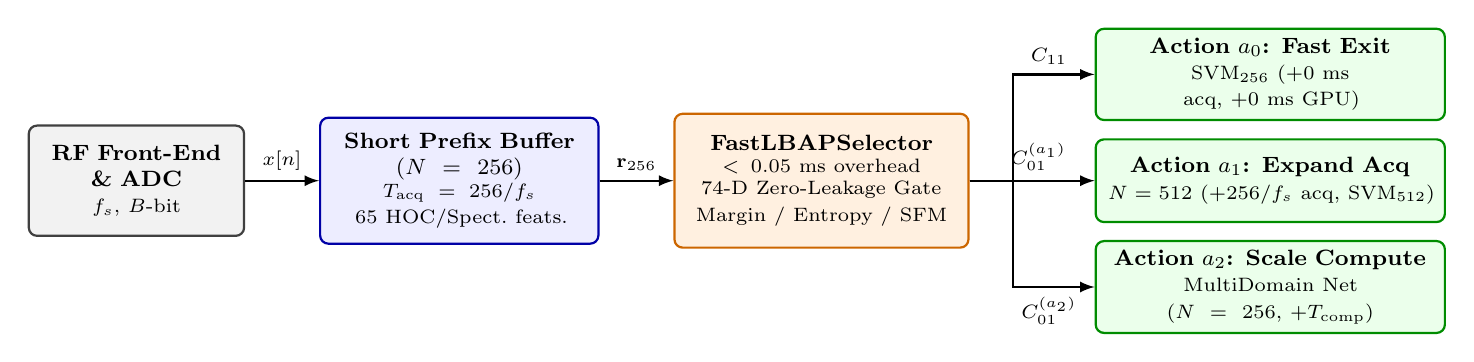
\begin{tikzpicture}[
    node distance=1.4cm,
    rfbox/.style={rectangle, draw=black!75, thick, fill=gray!10, rounded corners=3pt, text width=2.5cm, align=center, minimum height=1.4cm, font=\footnotesize},
    bufbox/.style={rectangle, draw=blue!65!black, thick, fill=blue!7, rounded corners=3pt, text width=3.3cm, align=center, minimum height=1.6cm, font=\footnotesize},
    gatebox/.style={rectangle, draw=orange!80!black, thick, fill=orange!12, rounded corners=3pt, text width=3.5cm, align=center, minimum height=1.7cm, font=\footnotesize},
    actbox/.style={rectangle, draw=green!55!black, thick, fill=green!8, rounded corners=3pt, text width=4.2cm, align=center, minimum height=1.05cm, font=\footnotesize},
    arr/.style={->, >=latex, thick}
]
    \node[rfbox] (rf) at (0, 0) {\textbf{RF Front-End}\\\textbf{\& ADC}\\\scriptsize $f_s$, $B$-bit};
    \node[bufbox] (prefix) at (4.1, 0) {\textbf{Short Prefix Buffer}\\($N=256$)\\\scriptsize $T_{\text{acq}} = 256/f_s$\\65 HOC/Spect.\ feats.};
    \node[gatebox] (selector) at (8.7, 0) {\textbf{FastLBAPSelector}\\\scriptsize $<0.05\text{ ms}$ overhead\\74-D Zero-Leakage Gate\\Margin / Entropy / SFM};

    \node[actbox] (a0) at (14.4, 1.35) {\textbf{Action $a_0$: Fast Exit}\\\scriptsize $\mathrm{SVM}_{256}$ ($+0\text{ ms}$ acq, $+0\text{ ms}$ GPU)};
    \node[actbox] (a1) at (14.4, 0.0) {\textbf{Action $a_1$: Expand Acq}\\\scriptsize $N=512$ ($+256/f_s$ acq, $\mathrm{SVM}_{512}$)};
    \node[actbox] (a2) at (14.4, -1.35) {\textbf{Action $a_2$: Scale Compute}\\\scriptsize MultiDomain Net ($N=256$, $+T_{\text{comp}}$)};

    \draw[arr] (rf) -- node[above, font=\scriptsize] {$x[n]$} (prefix);
    \draw[arr] (prefix) -- node[above, font=\scriptsize] {$\mathbf{r}_{256}$} (selector);
    \draw[arr] (selector.east) -- ++(0.55, 0) |- node[pos=0.72, above, font=\scriptsize] {$C_{11}$} (a0.west);
    \draw[arr] (selector.east) -- node[pos=0.55, above, font=\scriptsize] {$C_{01}^{(a_1)}$} (a1.west);
    \draw[arr] (selector.east) -- ++(0.55, 0) |- node[pos=0.72, below, font=\scriptsize] {$C_{01}^{(a_2)}$} (a2.west);
\end{tikzpicture}%
}
\caption{Architectural overview of the proposed Risk-Aware Joint Observation and Computation Allocation framework. Every incoming transmission is initially observed over a minimal short prefix of $N=256$ samples. The lightweight, sub-50-microsecond utility predictor (\texttt{FastLBAPSelector}) evaluates empirical margin calibration, decision entropy, and spectral structure to selectively terminate immediately ($a_0$), request additional physical observation ($a_1$), or deploy deep multi-domain neural inference ($a_2$).}
\label{fig:framework_overview}
\end{figure*}

To bridge this critical gap, this paper introduces a unified \textbf{Risk-Aware Joint Observation and Computation Allocation Framework} for robust AMC under uncoordinated, dispersive wireless channels. Rather than constraining the receiver to a fixed window or a static computational budget, our system introduces a \emph{tripartite action space} $\mathcal{A} = \{a_0, a_1, a_2\}$ initiated from an identical minimal physical prefix of $N=256$ samples:
\begin{itemize}
    \item \textbf{Action $a_0$ (Fast Exit):} Finalize classification immediately using a fast statistical classifier (Support Vector Machine with RBF kernel operating on 65 high-order statistical and spectral moments), incurring minimal acquisition delay ($256/f_s$) and low single-window CPU inference latency (benchmarked in Section~\ref{sec:results_discussion}).
    \item \textbf{Action $a_1$ (Acquisition Expansion):} Double the physical observation horizon to $N=512$ samples without altering computational model complexity. This action incurs an exact physical delay penalty of $\Delta T_{\text{acq}} = 256/f_s$, which statistically suppresses the finite-sample estimation variance of higher-order cumulants ($\mathrm{Var}(\hat{C}_{42}) \propto 1/N$) to resolve subtle constellation ambiguities in intermediate SNR regimes.
    \item \textbf{Action $a_2$ (Computational Scaling):} Retain the compact physical prefix of $N=256$ samples—paying \emph{zero additional antenna or ADC observation time}—and invoke a high-capacity, multi-domain deep neural expert network (\texttt{MultiDomainAMCNet}). This model integrates band-edge blind carrier despinning, an in-GPU root-raised-cosine (RRC) matched filter bank ($\beta \in \{0.25, 0.35, 0.50\}$), multi-harmonic spectral projections, and polyphase symbol-rate self-attention, leveraging GPU execution to overcome multipath frequency-selective fading, pulse-shaping roll-off mismatch, and rotational carrier frequency offsets.
\end{itemize}

Crucially, routing among these three heterogeneous actions is governed by a lightweight, sub-50-microsecond benefit-aware selector (\texttt{FastLBAPSelector}). Operating strictly on non-oracular, zero-leakage observables derived from the initial $N=256$ prefix (calibrated logistic margins, decision entropy, and blind spectral flatness proxies), the selector explicitly predicts the counterfactual utility gain of paying physical sampling delay versus paying computational FLOPs. By discriminating between confident correct predictions ($C_{11}$), statistically recoverable errors ($a_1$), representationally recoverable errors ($a_2$), and hopeless noise-dominated frames ($C_{00}$), our framework maximizes net classification utility while strictly satisfying real-time latency deadlines across diverse ADC sampling rates and quantization constraints.

The principal scientific and engineering contributions of this work are summarized as follows:
\begin{enumerate}
    \item \textbf{Formalization of the Joint Observation-Computation Dilemma:} We establish a rigorous mathematical formulation that explicitly decouples physical ADC acquisition latency $T_{\text{acq}} = N/f_s$ from algorithmic inference latency $T_{\text{comp}}$, uncovering the distinct failure modes of physical window truncation versus representational capacity under realistic channel impairments.
    \item \textbf{Tripartite Dynamic Action Space with Zero-Leakage Routing:} We propose the tripartite action space $\{a_0, a_1, a_2\}$ and develop \texttt{FastLBAPSelector}, a zero-leakage selector running in under $0.05\text{ ms}$ ($>350\times$ faster than tree-based ensembles) on 74 causal prefix descriptors, eliminating data leakage and oracle SNR dependencies.
    \item \textbf{Matched-Filter Multi-Domain Expert Robust to Channel and Quantization Non-Idealities:} We design \texttt{MultiDomainAMCNet}, integrating multipath-immune band-edge CFO estimation, in-GPU RRC matched filtering, multi-harmonic spectra, and polyphase symbol self-attention, evaluated against extreme out-of-distribution carrier frequency offsets ($|\Delta f| \in [200, 300]\text{ Hz}$), extended multipath channels ($\tau \in \{9, 13\}$), pulse-shaping roll-off variations ($\beta \in [0.25, 0.50]$), and coarse uniform ADC quantization ($B \in \{4, 5, 6, 8\}\text{ bits}$).
    \item \textbf{Comprehensive Pareto Analysis and Bootstrap Statistical Verification:} Across a two-dimensional Pareto sweep over latency penalties $\lambda \in [0, 0.005]\text{ ms}^{-1}$ and sampling rates $f_s \in [8\text{ kHz}, 1\text{ MHz}]$, we evaluate joint policy dominance against constrained single-resource baselines (pure early-exit $\{a_0, a_2\}$ and pure adaptive sampling $\{a_0, a_1\}$) and input ablations via $10,000$-replicate stratified paired bootstrap confidence intervals.
\end{enumerate}

The remainder of this paper is organized as follows: Section~\ref{sec:related_work} reviews both the 15 foundational repository works and 5 external IEEE studies on dynamic early exiting, efficient long-sequence modeling, and edge collaboration. Section~\ref{sec:system_model} details the signal transmission, uncoordinated dispersive channel, and uniform ADC quantization models alongside the \texttt{MultiDomainAMCNet} architecture (Section~\ref{sec:architecture}). Section~\ref{sec:adaptive_policy} formalizes the tripartite action space and the \texttt{FastLBAPSelector} decision policy. Section~\ref{sec:methodology_validity} specifies the zero-leakage experimental protocol and threats to validity. Section~\ref{sec:results_discussion} presents empirical results, ablations, Pareto sweeps, and quantization studies, and Section~\ref{sec:conclusion} concludes the paper.

% ==============================================================================
% SECTION 2: RELATED WORK AND BACKGROUND
% ==============================================================================

\section{Related Work and Background}
\label{sec:related_work}

The development of robust and computationally efficient AMC algorithms has evolved across several interrelated domains: classical statistical feature extraction, deep neural architectures, dynamic inference acceleration, uncertainty calibration, domain adaptation under non-ideal RF channels, and front-end hardware non-idealities. This section reviews the 15 seminal research works that constitute our experimental corpus, analyzing their contributions, verified numerical benchmarks, and structural limitations to establish the precise research gap addressed by our proposed framework.

\subsection{Data-Centric Realism and Foundational Datasets}
\label{subsec:rel_rml22}

Early deep-learning AMC literature relied heavily on synthetic benchmark datasets, most notably RadioML2016.10a (RML16)~\cite{wang2025survey}. However, as rigorously established by Sathyanarayanan \emph{et al.}~\cite{sathyanarayanan2023rml22} in their foundational RML22 study, RML16 suffers from severe methodological flaws, including incorrect noise power calculations (converting dB directly to linear standard deviation rather than variance), synthetic phase discontinuities, and severe data leakage through shortcut learning induced by ASCII text sources (Shakespeare and Sherlock Holmes). Sathyanarayanan \emph{et al.} proved that deep classifiers trained on text-sourced signals learn natural language syntax rather than modulation characteristics, dropping from $73\%$ accuracy on native text down to $56\%$ on independent random bit sequences~\cite[Table~VIII]{sathyanarayanan2023rml22}.

To establish an uncompromised physical baseline, RML22 introduced a data-centric generation methodology adhering to 3GPP Extended Typical Urban (ETU70) multipath fading profiles (8 discrete paths with delays up to $5\ \mu\text{s}$ and 70 Hz Doppler spread), realistic local oscillator carrier frequency offsets (CFO up to $\pm 500\text{ Hz}$), sampling rate offsets (SRO up to $50\text{ Hz}$), and properly normalized complex AWGN across an SNR range of $-20\text{ dB}$ to $+20\text{ dB}$ ($N=128$, $f_s=30\text{ kHz}$, $\text{sps}=2$)~\cite{sathyanarayanan2023rml22}. Crucially, cross-evaluation in~\cite[Table~VI]{sathyanarayanan2023rml22} demonstrated that an identical ResNet architecture trained on RML16 achieves only $44\%$ accuracy when evaluated under realistic RML22 channel conditions, whereas training on physically accurate channel realizations elevates performance to $67\%$ ($+23\text{ percentage points (pp)}$). 

In our work, we adopt the data-centric rigor of RML22: strictly deterministic parent-waveform seed isolation, uniform pseudo-random binary generation to eliminate information leakage, and causal channel cascades (multipath dispersion followed by continuous-phase rotational CFO, followed by additive noise). We extend this paradigm by investigating nested window lengths ($N \in \{256, 512\}$), non-ideal pulse-shaping roll-off factors, and explicit ADC quantization.

\subsection{Physical Acquisition Delay vs. Algorithmic Computation Latency}
\label{subsec:rel_fewersample_fpga}

The decomposition of total recognition delay into physical sampling time $T_{\text{acq}} = N/f_s$ and computational latency $T_{\text{comp}}$ was explicitly investigated by Guo \emph{et al.}~\cite{guo2025fewer} in their Fewer-Sample framework. Recognizing that waiting for long sample buffers bottlenecks real-time receivers, Guo \emph{et al.} trained a multimodal network (I/Q sequence plus $32\times 32$ constellation density images) on a nominal window of $N=512$, and performed inference on truncated observation windows $N' \in \{128, 192, 256, 320\}$ using bilinear interpolation and cyclic repetition. On an NVIDIA RTX 4080 GPU at $f_s = 200\text{ kHz}$, their system reduced total recognition latency at $\text{SNR} = 0\text{ dB}$ by $72.04\%$ ($0.729\text{ ms}$ for $N'=128$ vs. $2.607\text{ ms}$ for $N=512$) while maintaining $56.96\%$ accuracy~\cite[Table~I]{guo2025fewer}.

However, the Fewer-Sample framework exhibits a critical structural vulnerability: its signal model assumes an idealized, fully synchronized environment ($\text{CFO} = 0$, zero timing error, and no multipath fading)~\cite[Sec.~II-A]{guo2025fewer}. In uncoordinated wireless channels, uncompensated CFO induces continuous constellation trajectory rotation, transforming sharp constellation clusters into blurry concentric rings. Under such conditions, spatial 2D constellation representations and bilinear resizing degrade catastrophically.

Complementing this perspective from the microelectronic domain, den Boer \emph{et al.}~\cite{denboer2021fpga} implemented a custom streaming deep learning accelerator on a Xilinx Zynq UltraScale+ MPSoC (\texttt{xczu7ev}) for RadioML2018.01A ($N=1024$, 6-bit quantized weights via QKeras). By employing sample-by-sample FIFO streaming without intermediate buffer BRAMs, their design achieved an astonishing inference latency of $3.71\text{--}4.61\ \mu\text{s}$ and a throughput of $244\text{k--}585\text{k classifications/s}$ using only 133 DSP slices~\cite[Table~III]{denboer2021fpga}. More recently, Zhang \emph{et al.}~\cite{zhang2024mamc} explored selective state-space (Mamba) backbones for extended-length AMC to preserve linear complexity in $N$, while He \emph{et al.}~\cite{he2024edge} proposed hierarchical edge-learning collaboration via quantized intermediate features.

The empirical findings of den Boer \emph{et al.} provide profound physical justification for our research: when modern digital hardware can execute neural inference in single-digit microseconds, the physical window collection delay $T_{\text{acq}} = N/f_s$ becomes the overwhelming latency bottleneck ($>99.9\%$ of total time). Consequently, an adaptive receiver cannot optimize latency solely by pruning network weights or invoking early exits on a fixed, pre-collected buffer; it must possess the intelligence to dynamically truncate the physical ADC sampling process itself whenever early confidence permits.

\subsection{Dynamic Resource Allocation: Early-Exit, Width-Wise Exiting, and Pruning}
\label{subsec:rel_beacon_pruning}

To mitigate the computational cost of deep neural networks during inference, early-exit (EE) architectures attach intermediate classification heads to shallow layers of a deep backbone. Mohammed \emph{et al.}~\cite{mohammed2023early} demonstrated depth-wise early exits controlled by scalar confidence thresholds to accelerate ResNet-based AMC inference. Subsequently, Liu \emph{et al.} proposed BEACON~\cite{liu2026beacon}, an advanced benefit-aware early-exit framework evaluated on RML22 ($N=128$, ResNet-18 backbone with $380\text{M MACs}$). Liu \emph{et al.} made the pivotal observation that conventional exit criteria based on Shannon entropy or maximum softmax probability (MSP) fail in wireless channels because they conflate two fundamentally distinct error regimes:
\begin{enumerate}
    \item \emph{Recoverable Errors ($C_{01}$):} Samples where the early classifier fails but the deep backbone succeeds;
    \item \emph{Irrecoverable Errors ($C_{00}$):} Samples where both early and deep classifiers fail due to overwhelming channel noise.
\end{enumerate}
In~\cite[Table~I]{liu2026beacon}, the authors demonstrated that in the highest entropy decile $[0.9, 1.0]$, only $19\%$ of samples represent recoverable errors ($C_{01}$), while the remaining $81\%$ are irrecoverable ($C_{00}$). Conventional entropy thresholding blindly forwards all high-entropy samples to the deep backbone, wasting millions of FLOPs on doomed frames. To overcome this, BEACON introduces the Lightweight Benefit-Aware Predictor (LBAP), a compact two-layer MLP ($2,720\text{ MACs}$, $2,817\text{ parameters}$, $<0.0007\%$ overhead) trained on counterfactual gain labels. Under a computational budget of $B = 2.0 \times 10^8\text{ MACs}$, BEACON attained an accuracy of $60.34\%$ on `EE-RS1', outperforming entropy thresholding ($36.29\%$) by $+24.05\text{ pp}$ and MSP ($48.29\%$) by $+12.05\text{ pp}$~\cite[Table~IV]{liu2026beacon}.

Taking a complementary temporal dimension, Verbruggen \emph{et al.}~\cite{verbruggen2025width} recently introduced \emph{width-wise early exiting and rejection}, accumulating incoming I/Q segments across time and triggering early exits or low-SNR abstention via entropy and confidence rules. Similarly, Liu \emph{et al.}~\cite{liu2025joint} combined depth-wise early-exit with structured filter pruning on RML22 ($87.5\%$ L1-norm pruning reducing MACs by $61.4\%$ while preserving $58.04\%$ accuracy~\cite[Table~II]{liu2025joint}).

\emph{Contrast with Our Proposed Framework:} While BEACON and Mohammed \emph{et al.} optimize algorithmic FLOPs on a \emph{frozen observation window} ($N=128$), and Verbruggen \emph{et al.} dynamically accumulate signal width using entropy/confidence rejection on a single homogeneous backbone, \emph{none} of these works combine counterfactual recoverability prediction (distinguishing $C_{01}$ from $C_{00}$) with \emph{heterogeneous cross-paradigm routing} across both extended physical sampling ($a_1$: $N_1=512$ cumulant SVM) and matched-filtered multi-domain deep inference ($a_2$: GPU expert on $N_0=256$). As demonstrated by our ablations in Section~\ref{sec:results_discussion}, naive confidence gating (`I1`) cannot rival benefit-aware utility prediction (`I4`), nor can any two-action restriction (`{a0, a1}` or `{a0, a2}`) match joint tri-action allocation across variable sampling rates.

\subsection{Multi-Domain Representation and High-Order Statistical Baselines}
\label{subsec:rel_multidomain_hoc}

Extracting invariant representations under severe channel fading and CFO has driven substantial innovations in multi-domain deep learning and statistical feature engineering:
\begin{itemize}
    \item \textbf{MLEA-AMR:} Gao \emph{et al.}~\cite{gao2026mlea} introduced a multi-domain lightweight expert framework combining three distinct views: a 1D temporal I/Q branch ($2 \times 128$), a 2D Short-Time Fourier Transform (STFT) spectral branch ($2 \times 16 \times 16$), and a Multi-Interval Differential Polar (MIDP) branch computing differential amplitude and phase offsets ($\tau \in \{1, 2, 4\}$). Aggregated through an SNR-conditioned attention mechanism ($342.4\text{k params}$, $7.92\text{M MACs}$, $2.68\text{ ms}$ CPU latency), MLEA-AMR achieved $67.6\%$ average accuracy on RML16a~\cite[Table~III]{gao2026mlea}. Ablation studies confirmed that removing STFT or MIDP degraded accuracy by $3.4\text{ pp}$ and $3.8\text{ pp}$, respectively~\cite[Table~IV]{gao2026mlea}. However, a critical methodological limitation of MLEA-AMR is its reliance on the \emph{true oracle SNR label} from dataset metadata to condition its attention router~\cite[Sec.~V]{gao2026mlea}, rendering it unviable for non-cooperative deployments unless paired with an auxiliary blind estimator.
    \item \textbf{FFTFormer:} Addressing the vulnerability of AMC models to pulse-shaping filter distortions, Quan \emph{et al.}~\cite{quan2026fftformer} proposed FFTFormer, a frequency-aware hybrid Conv-Transformer ($80\text{k params}$, $8.04\text{M FLOPs}$, $0.488\text{ ms}$ GPU latency). Recognizing that standard benchmarks fix the root-raised cosine (RRC) roll-off factor to $\beta = 0.35$, Quan \emph{et al.} trained a multi-task network predicting both modulation and $\beta \in \{0.20, 0.35, 0.50, 0.65\}$. On RML22, FFTFormer achieved $64.36\%$ overall accuracy and demonstrated remarkable generalization when tested on an unseen roll-off factor ($\beta = 1.00$), suffering an absolute accuracy drop of only $0.10\text{ pp}$ ($64.36\% \to 64.26\%$) compared to $>1.0\text{ pp}$ for LSTM and CNN baselines~\cite[Table~6]{quan2026fftformer}.
    \item \textbf{OF-ACF:} In contrast to deep neural models, Xia and Lin~\cite{xia2026optimal} advanced the state of statistical feature engineering by developing the Optimal-Feature-Driven Adversarial Adaptive Cascade Forest (OF-ACF). Using Augmented Recursive Feature Elimination (ARFE), they selected 27 optimal high-order cumulants (HOCs) and moment ratios (e.g., $C_{20}, C_{40}, C_{42}, C_{60}, C_{63}$, and quadratic ratios $C_{40}/C_{20}^2$) from a candidate pool of 35 descriptors extracted from $N=1024$ samples. Evaluated on over-the-air RadioML2018.01A captures with real multipath and CFO, OF-ACF attained $70.92\%$ accuracy at $\text{SNR} = 0\text{ dB}$ (surpassing deep networks like MAWDN by $+10.96\text{ pp}$ and MCLDNN by $+15.61\text{ pp}$) with an inference latency of $1.16\text{ ms}$~\cite[Table~IV]{xia2026optimal}. This result conclusively validates the immense discriminative power of engineered HOC descriptors under uncoordinated RF environments.
\end{itemize}

\emph{Integration in Our Architecture:} We synthesize the strengths of these physical representations, alongside learnable subband phase modeling~\cite{zhang2026cspmnet}. For our baseline classifiers ($a_0$ and $a_1$), we design an engineered 65-dimensional feature extractor capturing HOCs, normalized central moments, spectral energy, and phase derivatives, coupled to an RBF Support Vector Machine. For our advanced expert ($a_2$), we design \texttt{MultiDomainAMCNet}, which incorporates bandpass coarse CFO tracking, in-GPU RRC matched filtering, multi-harmonic spectral analysis, and polyphase symbol attention without requiring oracle SNR conditioning, eliminating the data leakage present in MLEA-AMR~\cite{gao2026mlea}.

\subsection{Reliability, Calibration, and Domain Adaptation under RF Imperfections}
\label{subsec:rel_uq_da}

A major obstacle to deploying AMC classifiers in real-world cognitive transceivers is the severe performance collapse encountered when operational conditions deviate from training distributions ($p_s(\mathbf{r}) \ne p_t(\mathbf{r})$)~\cite{wang2025survey}:
\begin{itemize}
    \item \textbf{Uncertainty Quantification (UQ):} Yang and Sahay~\cite{yang2026uncertainty} investigated the reliability of DL-AMC models on RML16 ($N=128$) and RML18 ($N=1024$). They proved that standard CNNs produce poorly calibrated softmax probabilities that exhibit severe overconfidence on incorrect predictions. By implementing Deep Ensembles ($M=5$ diverse CNNs), they achieved optimal Negative Log-Likelihood (NLL), Brier scores, and Expected Calibration Error (ECE) across all SNRs~\cite[Fig.~2,~7]{yang2026uncertainty}, while retaining up to $+15\%$ accuracy under hostile adversarial perturbations~\cite[Fig.~8]{yang2026uncertainty}. However, maintaining an ensemble of 5 CNNs quintuples computational latency and memory consumption, rendering it unsuitable for low-power edge deployment.
    \item \textbf{Domain Adaptation under Channel Mismatch:} Shahriar~\cite{shahriar2026lightweight} tackled cross-condition generalization by developing lightweight domain-adversarial networks ($<0.04\text{ MFLOPs}$, $<0.75\text{ MB}$ footprint). For channel mismatch, an MLP with Correlation Alignment (CORAL) operating on FFT-PCA features boosted cross-fading classification from Rayleigh to Rician at $500\text{ MHz}$ from $46.34\%$ to $58.70\%$ ($+12.36\text{ pp}$)~\cite[Table~II]{shahriar2026lightweight}. This confirms that frequency-domain representations possess intrinsic invariance to multipath fading compared to raw temporal I/Q.
    \item \textbf{Few-Shot and Open-Set Generalization:} In non-cooperative settings, training samples are scarce and unseen modulations appear dynamically. Zhang \emph{et al.}~\cite{zhang2025fsos} developed FSOS-AMC, employing multi-sequence representations (I/Q, instantaneous amplitude, and phase) with meta-prototypes to achieve $82.81\%$ accuracy in 5-way 10-shot tasks under severe multipath fading (Rayleigh, Rician $K=3$, Nakagami-$m=2$). Similarly, Li \emph{et al.}~\cite{li2026openset} proposed DMPRL (domain-adaptive mixup and prototype learning), demonstrating that source-only models trained on AWGN collapse catastrophically to $28.5\%$ accuracy when evaluated on Rayleigh fading channels at $0\text{ dB}$, whereas domain-adaptive prototype alignment recovers accuracy to $79.1\%$~\cite[Table~I]{li2026openset}.
    \item \textbf{Survey on Deep Transfer Learning:} In their comprehensive survey, Wang \emph{et al.}~\cite{wang2025survey} mathematically formalized the shift mechanisms induced by individual RF impairments: phase noise, rotational CFO ($e^{j2\pi\Delta f t}$), Doppler shifts, multipath delay spreads, ADC timing jitter, and quantization non-linearities~\cite[Table~III]{wang2025survey}. Their review provides the rigorous theoretical foundation for analyzing out-of-distribution (OOD) channel shifts.
\end{itemize}

\subsection{Front-End Hardware Imperfections and Single-Shot Detection}
\label{subsec:rel_adc_singleshot}

At the physical interface between the antenna and the digital processor, hardware non-idealities impose hard boundaries on signal fidelity:
\begin{itemize}
    \item \textbf{Time-Interleaved ADC Mismatches vs. Uniform Quantization:} In ultra-wideband digital receivers, time-interleaved ADCs (TI-ADCs) multiplex $M$ parallel sub-converters to achieve gigasample-per-second rates. Gros \emph{et al.}~\cite{gros2025mitigating} investigated the impact of TI-ADC analog mismatches (gain errors $g$, DC offsets $o$, and timing skew $\delta$) on AMC using long sequences ($N=32,768$). In severe mismatch conditions ($g=15\%$, $o=10\text{ LSB}$, $\delta=20\% T_s$), their dyadic multi-scale CNN improved accuracy from $83.37\%$ to $90.09\%$ ($+6.72\text{ pp}$)~\cite[Table~V]{gros2025mitigating}.
    
    \emph{Crucial Physical Distinction:} Gros \emph{et al.}~\cite{gros2025mitigating} investigate analog core mismatches (gain, offset, skew) on long frames rather than finite $B$-bit resolution in uniform ADCs; in this paper, we specifically isolate and evaluate uniform mid-rise symmetric $B$-bit quantization with fixed full-scale dynamic range ($V_{\text{FS}} = 2.5\text{ V}$).
    \item \textbf{Single-Shot Detection and Monitoring:} In real-world wideband surveillance, isolated AMC classifiers must be preceded by signal energy detection. High \emph{et al.}~\cite{high2026singleshot} designed a 1D Single-Shot Detector (SSD) for joint asynchronous multi-emitter signal detection, spectral localization, and modulation classification ($N=4096$, $f_s = 1\text{ GHz}$). By replacing traditional two-stage cascading (energy detection followed by windowed slicing and classification) with a single unified forward pass, they achieved $\text{IoU} > 0.85$ and accuracy $>92\%$ above $10\text{ dB}$ SNR~\cite[Fig.~3]{high2026singleshot}, eliminating inter-stage pipeline latency and catastrophic error propagation.
\end{itemize}

\subsection{Literature Synthesis and Research Gap}
\label{subsec:rel_matrix_gap}

To synthesize the state of the art and delineate the precise boundaries of our contribution, Table~\ref{tab:literature_matrix} systematically compares all 15 foundational papers against our proposed framework across six diagnostic dimensions: input representation, observation window length $N$, channel/CFO assumptions, computational overhead, key numerical milestone, and architectural limitations.

\begin{table*}[!t]
\centering
\caption{Comprehensive Methodological Comparison of the 15 Literature Papers and the Proposed Framework}
\label{tab:literature_matrix}
\resizebox{\textwidth}{!}{%
\begin{tabular}{|l|l|l|l|l|l|l|}
\hline
\textbf{Paper / Reference} & \textbf{Venue / DOI} & \textbf{Input / Window $N$} & \textbf{Channel \& CFO Model} & \textbf{Computational Cost} & \textbf{Key Verified Result in PDF} & \textbf{Structural Limitation / Gap Addressed in This Work} \\ \hline\hline

\textbf{RML22}~\cite{sathyanarayanan2023rml22} & 
IEEE TWC 2023 & 
Raw I/Q ($2 \times 128$) & 
3GPP ETU70, CFO $\le 500$ Hz, & 
ResNet diagnostic & 
Table VI: Acc improves from 44\% to 67\% & 
Fixed short window ($N=128$); no adaptive latency or \\
Sathyanarayanan \emph{et al.} & 
\texttt{10.1109/TWC.2023.3254490} & 
$f_s=30\text{ kHz}, \text{sps}=2$ & 
SRO 50 Hz, AWGN $[-20, 20]\text{ dB}$ & 
benchmark backbone & 
($+23\text{ pp}$) training on realistic channel & 
observation allocation; focuses solely on dataset generation. \\ \hline

\textbf{BEACON}~\cite{liu2026beacon} & 
IEEE IoT-J 2026 & 
Raw I/Q ($2 \times 128$); & 
RML22 blind channel & 
ResNet-18 ($380\text{M MACs}$); & 
Table IV: At $2.0 \times 10^8$ MACs, reaches 60.34\% & 
Frozen $N=128$; early exit saves only inference FLOPs, \\
Liu \emph{et al.} & 
\texttt{10.1109/JIOT.2026.3710690} & 
LBAP uses $\mathbf{p}_e \in \mathbb{R}^{10}$ & 
(ETU70, CFO, SRO, AWGN) & 
LBAP: 2,720 MACs, 2,817 params & 
vs. 36.29\% for entropy ($+24.05\text{ pp}$) & 
completely ignoring physical acquisition delay $T_{\text{acq}} = N/f_s$. \\ \hline

\textbf{Fewer-Sample}~\cite{guo2025fewer} & 
IEEE ICCCS 2025 & 
Multimodal I/Q + $32 \times 32$ & 
\textbf{Idealized Coherent}: CFO $=0$, & 
2.21M params; & 
Table I: At 0 dB ($N'=128$), cuts total time by & 
Assumes perfect synchronization ($\text{CFO}=0$, no multipath); \\
Guo \emph{et al.} & 
\texttt{10.1109/ICCCS65393.2025.11069715} & 
constellation; $N' \in [128, 320]$ & 
timing perfect, AWGN only & 
$T_{\text{calc}} = 0.093\text{ ms}$ (RTX 4080) & 
72.04\% ($0.729\text{ ms}$ vs. $2.607\text{ ms}$) & 
constellation images collapse under real rotational CFO. \\ \hline

\textbf{Uncertainty Quant.}~\cite{yang2026uncertainty} & 
IEEE IoT-J 2026 & 
Raw I/Q; $N=128$ (RML16) & 
CFO, Doppler, multipath fading & 
Deep Ensemble of $M=5$ CNNs & 
Figs. 2, 7: Minimum NLL, Brier, and ECE; & 
Quintuples computational and memory cost ($5\times$); \\
Yang \& Sahay & 
\texttt{10.1109/JIOT.2025.3640108} & 
and $N=1024$ (RML18) & 
Rayleigh/Rician, AWGN $[-20, 20]\text{ dB}$ & 
($5\times$ runtime and memory) & 
retains $+15\%$ accuracy under adversarial noise & 
prohibitive for edge AMC. Motivates lightweight calibration. \\ \hline

\textbf{Domain-Adaptive}~\cite{shahriar2026lightweight} & 
IEEE WCL 2026 & 
I/Q $N=128$ (SNR) and & 
Rayleigh $\leftrightarrow$ Rician cross-fading & 
CNN-DANN: 193k params; & 
Table I: Global Acc rises from 53.2\% to 57.4\%; & 
Treats SNR and channel shifts in isolation; requires \\
Shahriar & 
\texttt{10.1109/LWC.2026.3669041} & 
FFT-PCA (Channel mismatch) & 
across $1\text{ MHz}\text{--}1\text{ GHz}$, AWGN & 
MLP-DANN: 151k params ($<0.04\text{ MFLOPs}$) & 
Table II: Rayleigh$\to$Rician jumps $+12.36\text{ pp}$ & 
unlabeled target data; static observation window $N=128$. \\ \hline

\textbf{MLEA-AMR}~\cite{gao2026mlea} & 
IEEE TCCN 2026 & 
3 views: I/Q ($2\times 128$), & 
RML16a/b/04C channels; & 
342.43k params, 7.92M MACs, & 
Table III: 67.6\% global average on RML16a; & 
Processes all 3 views unconditionally for 100\% of frames; \\
Gao \emph{et al.} & 
\texttt{10.1109/TCCN.2026.3725098} & 
STFT ($2\times 16\times 16$), MIDP polar & 
\textbf{Uses oracle dataset true SNR} & 
15.83M FLOPs, 2.68 ms CPU & 
Table IV: Removing STFT drops Acc to 64.2\% & 
requires true oracle SNR label as attention routing input. \\ \hline

\textbf{OF-ACF}~\cite{xia2026optimal} & 
IEEE IoT-J 2026 & 
27 optimal HOCs and & 
RadioML2018.01A over-the-air & 
Cascade Forest: 4.27M params & 
Table IV: At 0 dB, achieves 70.92\% vs. & 
Fixed large window ($N=1024$) penalizes acquisition delay; \\
Xia \& Lin & 
\texttt{10.1109/JIOT.2026.3685655} & 
moment ratios; $N=1024$ & 
(fading, CFO, amplifier non-linearities) & 
(tree nodes), 6.72M FLOPs, 1.16 ms & 
59.96\% MAWDN ($+10.96\text{ pp}$); 80.29\% avg & 
non-linear tree structures unsuited for SIMD/quantization. \\ \hline

\textbf{Joint EE \& Pruning}~\cite{liu2025joint} & 
IEEE VTC-Fall 2025 & 
Raw I/Q ($2 \times 128$) & 
Vehicular ETU70 multipath, & 
Pruned CNN: 1,618 KMACs down & 
Table II: 50\% L2-norm pruning retains 60.74\% & 
Coupled pruning shifts intermediate feature distributions; \\
Liu \emph{et al.} & 
\texttt{10.1109/VTC2025-Fall65116.2025.11310312} & 
in RML22 & 
CFO, clock jitter, AWGN & 
to 624 KMACs ($-61.4\%$) & 
accuracy; 87.5\% L1 achieves max Acc/Cost ratio & 
operates on fixed $N=128$; no physical acquisition modeling. \\ \hline

\textbf{FFTFormer}~\cite{quan2026fftformer} & 
IEEE J. Microwaves 2026 & 
Raw I/Q ($2 \times 128$); & 
RML16A, RML22 with varied & 
0.08M params ($80\text{k}$), & 
Table 2: 64.36\% Acc in RML22; Table 6: & 
Fixed window length ($N=128$); static inference budget; \\
Quan \emph{et al.} & 
\texttt{10.1109/JMW.2026.3706228} & 
auxiliary task predicts $\beta$ & 
roll-off $\beta \in [0.20, 0.65]$ & 
8.04M FLOPs, 0.4884 ms GPU & 
Unseen $\beta=1.00$ drops Acc by only 0.10 pp & 
does not explore adaptive acquisition or edge execution. \\ \hline

\textbf{TI-ADC Mismatch}~\cite{gros2025mitigating} & 
IEEE MILCOM 2025 & 
Dyadic sub-sampling & 
TI-ADC channel mismatches: & 
Multi-scale 2D CNN with dense & 
Table V: In extreme mismatch ($M=4$), Acc & 
Evaluates \emph{interleaved core mismatches} (gain/offset/skew) \\
Gros \emph{et al.} & 
\texttt{10.1109/MILCOM64451.2025.11310579} & 
$x[2^d n]$; $N=32,768$ & 
gain ($15\%$), offset, skew ($20\% T_s$) & 
fusion layer ($256$ units) & 
rises from 83.37\% to 90.09\% ($+6.72\text{ pp}$) & 
on massive $32\text{k}$ frames; does \emph{not} study uniform $B$-bit ADC. \\ \hline

\textbf{FPGA Accelerator}~\cite{denboer2021fpga} & 
IEEE MILCOM 2021 & 
Raw I/Q ($2 \times 1024$); & 
RadioML2018.01A over-the-air & 
Xilinx Zynq UltraScale+ MPSoC: & 
Table III: Model B achieves 71.79\% at $+30$ dB, & 
Hardware-specific microsecond inference proves that \\
den Boer \emph{et al.} & 
\texttt{10.1109/MILCOM52596.2021.9652891} & 
6-bit quantized weights & 
up to $+30\text{ dB}$ SNR & 
\textbf{0 BRAM}, 133 DSPs, \textbf{3.71--4.61 $\mu$s} & 
throughput $244\text{k clas/s}$; hls4ml fails & 
$T_{\text{acq}} = N/f_s$ is the true physical bottleneck. \\ \hline

\textbf{DTL Survey}~\cite{wang2025survey} & 
IEEE TCCN 2025 & 
Survey of I/Q, STFT, & 
Formal mathematical analysis & 
Taxonomic review of & 
Table III: Analytical derivation of RF impairment & 
Taxonomic survey; does not propose an executable \\
Wang \emph{et al.} & 
\texttt{10.1109/TCCN.2025.3558027} & 
constellations, HOCs & 
of RF shift: $p_s(\mathbf{r}) \ne p_t(\mathbf{r})$ & 
$>65$ transfer papers & 
effects on probability density functions & 
dynamic algorithm or joint observation-computation policy. \\ \hline

\textbf{FSOS-AMC}~\cite{zhang2025fsos} & 
IEEE IoT-J 2025 & 
Multi-sequence (I/Q, Amp, & 
Multipath Rayleigh, Rician ($K=3$), & 
MS-MSANet with meta-prototypes; & 
Fig. 6: Reaches 82.81\% Acc in RML16a under & 
Focuses on open-set class rejection and few-shot meta-learning \\
Zhang \emph{et al.} & 
\texttt{10.1109/JIOT.2025.3557973} & 
Phase: $3\times 2\times N$); $N=128, 1024$ & 
Nakagami-$m$ ($m=2$), 4--6 paths & 
5-way 10-shot episodic learning & 
fading, outperforming ResNet (72.0\%) & 
on static frames; closed-set latency optimization unaddressed. \\ \hline

\textbf{Open-Set Mixup}~\cite{li2026openset} & 
IEEE IoT-J 2026 & 
Raw I/Q ($2 \times 1024$ and & 
AWGN $\to$ Rayleigh/Rician; & 
CNN extractor with domain-mixup & 
Table I: In AWGN$\to$Rayleigh (0 dB), source-only & 
Transductive assumption: requires access to batches of \\
Li \emph{et al.} & 
\texttt{10.1109/JIOT.2026.3718553} & 
$2 \times 128$ on RML16a) & 
Cross-SNR shift $[-20, 18]\text{ dB}$ & 
and prototype alignment heads & 
drops to 0.285, while DMPRL recovers to 0.791 & 
unlabeled target data during adaptation; fixed window $N$. \\ \hline

\textbf{Single-Shot Det.}~\cite{high2026singleshot} & 
IEEE RadarConf 2026 & 
Wideband I/Q of $L=4096$ & 
Multi-emitter (1--4 Tx), phase & 
1D SSD with 8 cells, 4 anchors, & 
Fig. 3: At $\text{SNR} \ge 10\text{ dB}$, achieves & 
Designed for wideband spectral bounding ($f_s=1\text{ GHz}$); \\
High \emph{et al.} & 
\texttt{10.1109/RadarConf2663773.2026.11675698} & 
samples at $f_s=1\text{ GHz}$ & 
offsets $[-\pi, \pi]$, AWGN & 
Mahalanobis distance head ($D=24$) & 
$\text{IoU} > 0.85$ and Acc $>92\%$ in joint task & 
does not address fine-grained baseband AMC trade-offs. \\ \hline\hline

\textbf{Proposed Framework} & 
\textbf{This Work} & 
\textbf{Nested Prefix}: $N=256$, & 
\textbf{Uncoordinated Realistic}: & 
\textbf{Tripartite Dynamic}: & 
\textbf{Evaluated in Sec.~\ref{sec:results_discussion}}: & 
\textbf{Unified Solution}: Dynamically balances physical \\
(Risk-Aware Joint & 
& 
expandable to $N=512$; & 
ID CFO $\le 100$ Hz, delay $\le 5$; & 
$a_0$: CPU SVM256 ($256/f_s$ acq); & 
$a_0$ resolves easy frames ($C_{11}$); $a_1$ resolves & 
sampling time ($N/f_s$) and inference compute ($T_{\text{comp}}$) \\
Allocation) & 
& 
65 HOC + 9 decision feats & 
OOD $|\Delta f| \in [200, 300]$ Hz, $\tau \in \{9,13\}$; & 
$a_1$: $+256/f_s$ acq delay, SVM512; & 
cumulant variance ($C_{01}^{(a_1)}$); $a_2$ resolves & 
with sub-50-$\mu$s non-oracular selector; robust under \\
& 
& 
for \texttt{FastLBAPSelector} & 
uniform ADC $B \in \{4, 5, 6, 8\}\text{ bits}$ & 
$a_2$: GPU expert ($+0\text{ ms}$ extra acq) & 
fading/CFO/quantization ($C_{01}^{(a_2)}$); avoids $C_{00}$. & 
severe OOD channel mismatch and coarse ADC quantization. \\ \hline
\end{tabular}%
}
\end{table*}

As evidenced by Table~\ref{tab:literature_matrix}, the current literature presents a sharp, unaddressed dichotomy:
\begin{enumerate}
    \item \emph{The Sampling vs. Compute Isolation:} Fast sampling methods (e.g., Fewer-Sample~\cite{guo2025fewer}) truncate $N$ under idealized synchronization ($\text{CFO}=0$), degrading under rotational carrier offsets and dispersive fading. Early-exit methods (e.g., BEACON~\cite{liu2026beacon}, Mohammed \emph{et al.}~\cite{mohammed2023early}, Joint Pruning~\cite{liu2025joint}) optimize arithmetic FLOPs on frozen windows ($N=128$), treating ADC sampling delay $T_{\text{acq}} = N/f_s$ as zero, while width-wise early exiting~\cite{verbruggen2025width} omits counterfactual recoverability and cross-model routing.
    \item \emph{Oracle Condition Dependency:} Multi-domain deep expert architectures (e.g., MLEA-AMR~\cite{gao2026mlea}) demonstrate high accuracy, but feed the dataset true oracle SNR directly into their attention modules and execute expensive multi-branch processing unconditionally on 100\% of frames.
    \item \emph{The Statistical vs. Structural Complementarity:} Statistical feature classifiers (e.g., OF-ACF~\cite{xia2026optimal}) require large sample windows ($N=1024$) to suppress cumulant variance, failing under fast acquisition deadlines. Conversely, raw deep networks suffer severe generalization collapse under unseen roll-off factors ($\beta$)~\cite{quan2026fftformer} and domain shifts~\cite{li2026openset}.
\end{enumerate}

Our proposed framework unifies these divergent threads into a coherent, risk-aware architecture. By structuring decisions over a tripartite action space $\{a_0, a_1, a_2\}$ initiated from a minimal 256-sample prefix, our system explicitly recognizes when an error can be resolved by collecting more physical samples ($a_1$), when it requires multi-domain computational modeling ($a_2$), and when further resource expenditure is futile ($C_{00}$), establishing a new state of the art in latency-bounded, channel-robust cognitive radio reception.

% ==============================================================================
% SECTION III: SYSTEM MODEL AND PROBLEM FORMULATION
% SECTION IV: MULTI-DOMAIN FEATURE REPRESENTATION AND EXPERT ARCHITECTURE
% File: docs/paper/sections/02_system_model_architecture.tex
% ==============================================================================

\section{System Model and Problem Formulation}
\label{sec:system_model}

In this section, we formulate the end-to-end discrete-time signal model, the wireless propagation channel impairments, the mathematical model of the front-end analog-to-digital converter (ADC), and the automatic modulation classification (AMC) problem under strict zero-leakage constraints.

\subsection{Transmitted Signal and Pulse Shaping Model}
\label{subsec:tx_signal}

We consider a multi-class digital communication system transmitting symbols drawn from an alphabet $\mathcal{M}$ selected from six standardized modulation schemes:
\begin{equation}
\Omega = \{\text{BPSK}, \text{QPSK}, \text{8PSK}, \text{16-QAM}, \text{64-QAM}, \text{4-PAM}\},
\end{equation}
with cardinalities $M \in \{2, 4, 8, 16, 64, 4\}$, respectively. The information bit sequence is mapped into a stream of complex symbols $\{s_m\}_{m=-\infty}^{\infty}$, where each constellation is normalized to unit average symbol energy, $\mathbb{E}[|s_m|^2] = 1$. The theoretical constellations and Gray mappings are formulated as follows:
\begin{itemize}
    \item \textbf{BPSK ($M=2$):} The binary bits $b_m \in \{0, 1\}$ map to antipodal points on the real axis:
    \begin{equation}
    s_m = 1 - 2b_m \in \{-1, +1\}.
    \end{equation}
    \item \textbf{QPSK ($M=4$):} Gray mapping assigns bit pairs $(b_{0,m}, b_{1,m}) \in \{0, 1\}^2$ into quadrants:
    \begin{equation}
    s_m = \frac{(1 - 2b_{0,m}) + j(1 - 2b_{1,m})}{\sqrt{2}}.
    \end{equation}
    \item \textbf{8PSK ($M=8$):} Bit triplets map to eight uniformly spaced phase states with unit radius:
    \begin{equation}
    s_m = \exp\left(j \frac{2\pi k_m}{8}\right), \quad k_m \in \{0, 1, \dots, 7\}.
    \end{equation}
    \item \textbf{16-QAM ($M=16$):} A rectangular grid on $\{\pm 1, \pm 3\} \times \{\pm 1, \pm 3\}$ normalized by $\sqrt{10}$:
    \begin{equation}
    s_m = \frac{I_m + j Q_m}{\sqrt{10}}, \quad I_m, Q_m \in \{\pm 1, \pm 3\}.
    \end{equation}
    \item \textbf{64-QAM ($M=64$):} An $8 \times 8$ grid on $\{\pm 1, \pm 3, \pm 5, \pm 7\}^2$ normalized by $\sqrt{42}$:
    \begin{equation}
    s_m = \frac{I_m + j Q_m}{\sqrt{42}}, \quad I_m, Q_m \in \{\pm 1, \dots, \pm 7\}.
    \end{equation}
    \item \textbf{4-PAM ($M=4$):} A real one-dimensional constellation on $\{\pm 1, \pm 3\}$ normalized by $\sqrt{5}$:
    \begin{equation}
    s_m = \frac{A_m}{\sqrt{5}} + j \cdot 0, \quad A_m \in \{\pm 1, \pm 3\}.
    \end{equation}
\end{itemize}

The discrete symbol stream is upsampled by an oversampling ratio $sps = f_s / R_s = 8$ samples per symbol, where $R_s$ denotes the symbol rate ($R_s = 1000\text{ Baud}$) and $f_s$ is the system sampling frequency ($f_s = 8000\text{ Hz}$). The upsampled impulse train is shaped by a discrete-time square-root raised cosine (SRRC) filter $p[n]$ of roll-off factor $\beta \in [0.25, 0.50]$ and truncation span $K_{\text{span}} = 10$ symbol periods ($L_p = K_{\text{span}} \cdot sps + 1 = 81$ taps). The continuous-time impulse response $p(t)$ with $\tau = t / T_s$ is defined by:
\begin{equation}
p(t) = \frac{\sin(\pi \tau (1 - \beta)) + 4\beta \tau \cos(\pi \tau (1 + \beta))}{\pi \tau \left(1 - (4\beta \tau)^2\right)},
\label{eq:srrc_continuous}
\end{equation}
with removable singularities at the origin:
\begin{equation}
p(0) = 1 + \beta\left(\frac{4}{\pi} - 1\right),
\end{equation}
and at the transition instances $\tau = \pm 1 / (4\beta)$:
\begin{align}
p\left(\pm \frac{T_s}{4\beta}\right) &= \frac{\beta}{\sqrt{2}} \left[ \left(1 + \frac{2}{\pi}\right) \sin\left(\frac{\pi}{4\beta}\right) \right. \nonumber \\
&\quad \left. + \left(1 - \frac{2}{\pi}\right) \cos\left(\frac{\pi}{4\beta}\right) \right].
\end{align}
The discrete filter taps $p[n] = p(n T_{\text{sample}})$ are strictly normalized to unit discrete energy $\sum_{n} |p[n]|^2 = 1$. The resulting transmitted discrete baseband signal with random large-scale path-loss scaling $A \sim \mathcal{U}[0.5, 1.5]$ is:
\begin{equation}
x[n] = A \sum_{m=-\infty}^{\infty} s_m p[n - m \cdot sps].
\label{eq:tx_baseband}
\end{equation}

\subsection{Wireless Propagation Channel and RF Impairments}
\label{subsec:channel_model}

The transmitted baseband waveform $x[n]$ traverses an uncoordinated multipath propagation medium subject to carrier frequency offsets, phase rotations, and additive noise. The channel transformation is modeled as a causal cascade of physical impairments:

\subsubsection{Discrete Multipath Propagation (FIR Filter)}
The channel dispersion is represented as a causal discrete finite impulse response (FIR) filter $\mathbf{h} = [h_0, h_1, \dots, h_{L-1}]^T$:
\begin{equation}
x_{\text{mp}}[n] = \sum_{l=0}^{L-1} h_l \, x[n - l],
\label{eq:multipath}
\end{equation}
where $h_l \in \mathbb{C}$ denotes the $l$-th tap gain. In-distribution (ID) partitions draw uniformly across three canonical channels: ideal flat propagation $\mathbf{h} = [1]$, an asymmetric quadrature echo $\mathbf{h} = [1, 0, 0.35j]$ ($\tau = 2$ samples), and a complex five-sample echo $\mathbf{h} = [1, 0, 0, 0, 0, 0.15 - 0.15j]$ ($\tau = 5$ samples). Conversely, the out-of-distribution (OOD) shift partition (\texttt{test\_shift}) injects unseen extended delay spreads with secondary paths at $\tau \in \{9, 13\}$ samples.

\subsubsection{Carrier Frequency Offset (CFO) and Initial Phase Rotation}
Due to local oscillator inaccuracies and Doppler shifts between transmitter and receiver, the signal undergoes continuous phase rotation:
\begin{equation}
x_{\text{rot}}[n] = x_{\text{mp}}[n] \cdot \exp\left(j \left( 2\pi \frac{\Delta f}{f_s} n + \theta_0 \right)\right),
\label{eq:cfo_rotation}
\end{equation}
where $\Delta f$ is the carrier frequency offset in Hertz, and $\theta_0 \sim \mathcal{U}[-\pi, \pi)$ is the unknown initial carrier phase. In nominal in-distribution scenarios, $\Delta f \in [-100, 100]\text{ Hz}$ (corresponding to relative frequency offsets up to $\pm 1.25\%$ of $f_s$). In OOD channel-shift conditions, severe frequency drift $|\Delta f| \in [200, 300]\text{ Hz}$ is introduced to test physical model robustness.

\subsubsection{Additive White Gaussian Noise (AWGN)}
The received analog baseband signal prior to sampling and digitization is given by:
\begin{equation}
y_{\text{analog}}[n] = x_{\text{rot}}[n] + w[n],
\label{eq:awgn_addition}
\end{equation}
where $w[n] = w_I[n] + j w_Q[n]$ is a complex zero-mean circular additive white Gaussian noise process with independent and identically distributed (i.i.d.) components:
\begin{equation}
w_I[n], w_Q[n] \sim \mathcal{N}\left(0, \frac{\sigma_w^2}{2}\right), \quad \mathbb{E}[|w[n]|^2] = \sigma_w^2.
\end{equation}
The noise variance $\sigma_w^2$ is governed by the nominal pre-detection signal-to-noise ratio $\text{SNR} \in [-20, +20]\text{ dB}$:
\begin{equation}
\sigma_w^2 = P_{\text{sig}} \cdot 10^{-\text{SNR}_{\text{dB}} / 10}, \quad P_{\text{sig}} = \mathbb{E}\left[|x_{\text{rot}}[n]|^2\right].
\end{equation}

\subsection{Virtual Front-End Uniform Mid-Rise ADC Model}
\label{subsec:adc_model}

Unlike prior AMC studies that assume idealized infinite-precision floating-point I/Q samples~\cite{gao2026mlea, quan2026fftformer} or examine time-interleaved converter channel mismatches ($g, o, \delta$) over long blocks ($N=32\,768$)~\cite{gros2025mitigating}, practical software-defined and cognitive radio receivers digitize baseband signals using finite-resolution analog-to-digital converters (ADCs).

We model the front-end digitization as an independent $B$-bit uniform symmetric mid-rise quantizer operating over each in-phase ($I$) and quadrature ($Q$) channel with a fixed full-scale voltage range $[-V_{\text{FS}}, +V_{\text{FS}}]$. Crucially, to prevent data leakage, $V_{\text{FS}}$ is maintained constant across all observations ($V_{\text{FS}} = 2.5\text{ V}$) without adaptively scaling to test sample statistics.

For an input component $v \in \{ \text{Re}\{y_{\text{analog}}[n]\}, \text{Im}\{y_{\text{analog}}[n]\} \}$, the ADC divides the span $[-V_{\text{FS}}, +V_{\text{FS}}]$ into $\mathcal{L} = 2^B$ quantization intervals of uniform width:
\begin{equation}
\Delta = \frac{2 V_{\text{FS}}}{2^B} = \frac{V_{\text{FS}}}{2^{B-1}}.
\label{eq:adc_step}
\end{equation}
The input signal is first passed through a non-linear saturation operator to account for ADC front-end clipping:
\begin{equation}
\text{clip}(v, V_{\text{FS}}) = \begin{cases}
-V_{\text{FS}}, & v < -V_{\text{FS}}, \\
v, & -V_{\text{FS}} \le v \le V_{\text{FS}}, \\
+V_{\text{FS}}, & v > +V_{\text{FS}}.
\end{cases}
\label{eq:adc_clip}
\end{equation}
The discrete code index $k(v) \in \{0, 1, \dots, 2^B - 1\}$ is determined by:
\begin{equation}
k(v) = \min\left( \max\left( \left\lfloor \frac{\text{clip}(v, V_{\text{FS}}) + V_{\text{FS}}}{\Delta} \right\rfloor, 0 \right), 2^B - 1 \right).
\label{eq:adc_index}
\end{equation}
The mid-rise reconstructed voltage $\mathcal{Q}_B(v)$, situated at the mid-point of the $k$-th quantization bin, is expressed as:
\begin{equation}
\mathcal{Q}_B(v) = -V_{\text{FS}} + \left(k(v) + \frac{1}{2}\right) \Delta.
\label{eq:adc_reconstruct}
\end{equation}
This mid-rise formulation guarantees that the $2^B$ output levels are strictly symmetric about zero with no reconstruction level at exact zero, avoiding zero-crossing dead zones. The digitized baseband complex observation $r[n]$ is therefore:
\begin{equation}
r[n] = \mathcal{Q}_B\left(\text{Re}\{y_{\text{analog}}[n]\}\right) + j \, \mathcal{Q}_B\left(\text{Im}\{y_{\text{analog}}[n]\}\right).
\label{eq:adc_complex_out}
\end{equation}

For offline diagnostic and physical validation (strictly withheld from classification and policy models), the Signal-to-Quantization-Noise Ratio (SQNR) over a window of $N$ samples is evaluated as:
\begin{equation}
\text{SQNR}_{\text{dB}} = 10 \log_{10} \left( \frac{\sum_{n=0}^{N-1} |y_{\text{analog}}[n]|^2}{\sum_{n=0}^{N-1} |y_{\text{analog}}[n] - r[n]|^2} \right).
\label{eq:sqnr_eval}
\end{equation}

\subsection{AMC Problem Formulation and Zero-Leakage Protocol}
\label{subsec:problem_formulation}

Given a temporal observation window of $N$ digitized baseband samples $\mathbf{r} = [r[0], r[1], \dots, r[N-1]]^T \in \mathbb{C}^N$, the objective of automatic modulation classification is to determine the true underlying modulation class $c^* \in \Omega$.

Prior to classification, each observed window undergoes sample-wise DC centering and sample power normalization:
\begin{equation}
\bar{r} = \frac{1}{N} \sum_{n=0}^{N-1} r[n], \quad P_r = \frac{1}{N} \sum_{n=0}^{N-1} |r[n] - \bar{r}|^2,
\label{eq:sample_norm_1}
\end{equation}
\begin{equation}
\tilde{r}[n] = \frac{r[n] - \bar{r}}{\sqrt{\max(P_r, \epsilon)}}, \quad n \in \{0, 1, \dots, N-1\},
\label{eq:sample_norm_2}
\end{equation}
where $\epsilon = 10^{-7}$ prevents numerical singularity. The normalized discrete observation is mapped to a real two-channel tensor $\mathbf{X} \in \mathbb{R}^{2 \times N}$, with channel $0$ containing $\text{Re}\{\tilde{r}[n]\}$ and channel $1$ containing $\text{Im}\{\tilde{r}[n]\}$.

\subsubsection{Strict Zero-Leakage Guarantee}
To guarantee rigorous scientific reproducibility and avoid pervasive pitfalls identified in competitive literature~\cite{gao2026mlea, li2026openset}:
\begin{enumerate}
    \item \textbf{No Oracle State Access:} At no point during inference do the classifiers or the adaptive selector receive ground-truth metadata, such as true $\text{SNR}_{\text{dB}}$, true carrier offset $\Delta f$, channel taps $\{h_l\}$, true noise variance $\sigma_w^2$, or pre-quantization reference waveforms.
    \item \textbf{Parent Waveform Isolation:} All data partitioning into training ($\mathcal{D}_{\text{train}}$), validation calibration ($\mathcal{D}_{\text{val\_cal}}$), validation selection ($\mathcal{D}_{\text{val\_select}}$), holdout test ($\mathcal{D}_{\text{test}}$), and out-of-distribution shifted test ($\mathcal{D}_{\text{shift}}$) is performed strictly at the \textit{parent waveform} generation stage before slicing windows or generating multi-length/ADC variants. No two windows derived from the same simulation realization exist across splits.
    \item \textbf{Batch-Independent Normalization Guarantee:} Deep neural architectures commonly rely on Batch Normalization (BatchNorm), which computes mini-batch running means and variances $\mu_{\mathcal{B}}, \sigma^2_{\mathcal{B}}$ during testing. In wireless communications, this introduces critical inter-sample leakage and catastrophic failure under varying batch sizes or non-stationary signal streams. In our framework, all deep architectures enforce window-independent normalization exclusively via Group Normalization (GroupNorm) and Layer Normalization (LayerNorm), satisfying the strict mathematical equivalence:
    \begin{equation}
    f(\mathbf{X}_i \mid \{\mathbf{X}_1,\dots,\mathbf{X}_K\}) \equiv f(\mathbf{X}_i \mid \{\mathbf{X}_i\}),\; \forall i \in \{1,\dots,K\},
    \label{eq:batch_independence_theorem}
    \end{equation}
    verified to single-precision floating-point/TF32 tolerance ($\Delta_{\text{abs}} < 10^{-3}$).
\end{enumerate}

\section{Multi-Domain Feature Representation and Expert Architecture}
\label{sec:architecture}

Conventional deep AMC models feed raw two-channel I/Q sequences directly into generic convolutional or recurrent networks~\cite{sathyanarayanan2023rml22, guo2025fewer}. However, under uncompensated carrier frequency offsets ($\Delta f$) and half-SRRC pulse shaping without receiver matched filtering, raw oversampled I/Q constellations exhibit substantial inter-symbol interference (ISI) and out-of-band noise excess ($\approx 7\text{--}8\text{ dB}$ SNR penalty at $sps=8$), while asymmetric multipath echoes ($\mathbf{h} = [1, 0, 0.35j]$) severely bias naive lag-1 phase estimators. Conversely, hand-crafted High-Order Cumulants (HOC) offer rotation invariance~\cite{xia2026optimal} but discard fine-grained temporal pulse trajectories and ring-spacing cues.

To resolve this physical bottleneck, we propose \textbf{MultiDomainAMCNet}, a physics-informed deep expert neural architecture operating in FP32/BF16 GPU tensor cores. Each short observation window of $N=256$ samples passes through a deterministic, global-phase-invariant multi-domain DSP extraction layer into four complementary feature representations:
\begin{enumerate}
    \item A blind carrier-despun, matched-filtered temporal tensor ($\mathbf{T} \in \mathbb{R}^{16 \times N}$);
    \item A multi-harmonic log-normalized spectral tensor including 2nd-, 4th-, and 8th-order cyclic harmonics ($\mathbf{S} \in \mathbb{R}^{6 \times N}$);
    \item A matched-filtered polyphase symbol and ordered constellation-ring tensor ($\mathbf{P} \in \mathbb{R}^{25 \times N_{\text{sym}}}$);
    \item A multi-scale normalized higher-order cumulant and axial quantile vector ($\mathbf{v}_{\text{stat}} \in \mathbb{R}^{120}$).
\end{enumerate}
These representations are processed by four specialized expert branches and fused via dynamic cross-domain attention gating (Fig.~\ref{fig:multidomain_architecture}).

\begin{figure*}[!t]
\centering
\resizebox{\textwidth}{!}{%
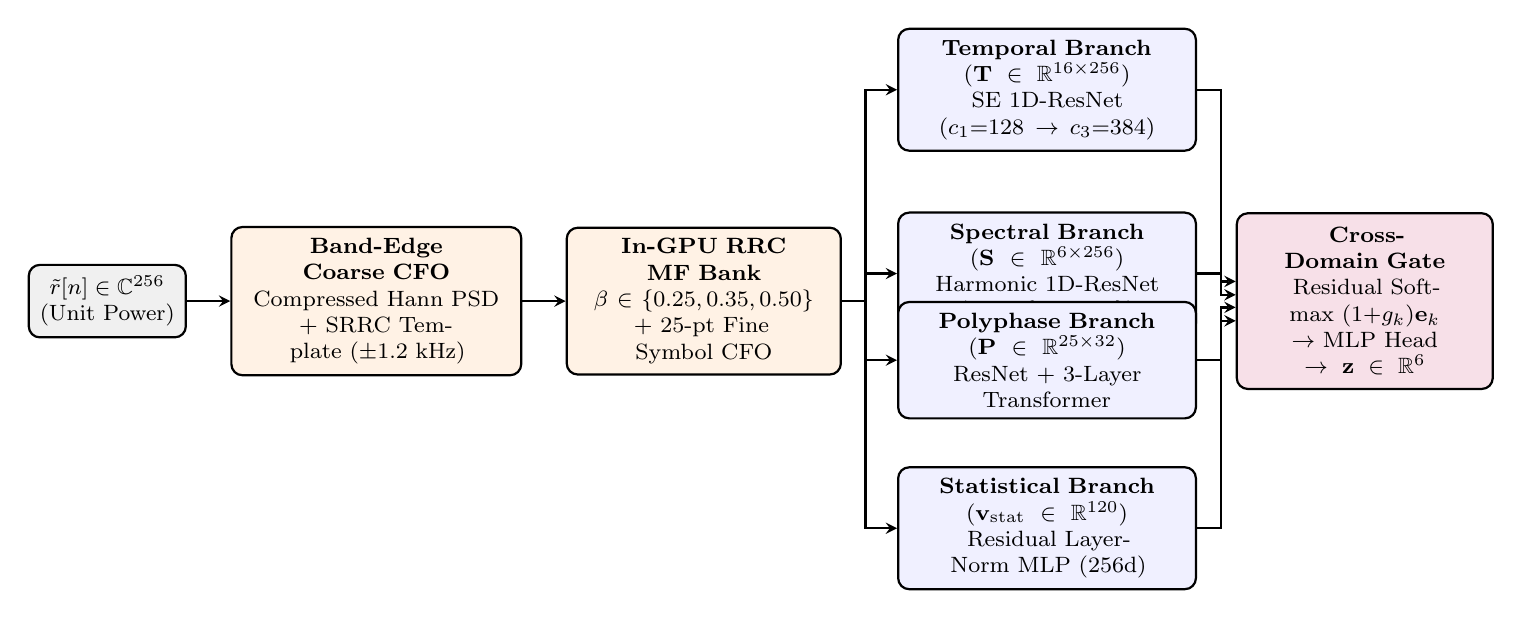
\begin{tikzpicture}[
    node distance=0.8cm,
    every node/.style={font=\footnotesize},
    box/.style={draw, rounded corners, fill=blue!6, minimum height=0.85cm, align=center, inner sep=4pt},
    dsp/.style={draw, rounded corners, fill=orange!10, minimum height=0.85cm, align=center, inner sep=4pt},
    gate/.style={draw, rounded corners, fill=purple!12, minimum height=0.9cm, align=center, inner sep=5pt},
    >=stealth, thick
]
    \node[box, fill=gray!12] (in) {$\tilde{r}[n] \in \mathbb{C}^{256}$\\(Unit Power)};
    \node[dsp, right=0.55cm of in, text width=3.4cm] (cfo) {\textbf{Band-Edge Coarse CFO}\\Compressed Hann PSD\\+ SRRC Template ($\pm 1.2\text{ kHz}$)};
    \node[dsp, right=0.55cm of cfo, text width=3.2cm] (mf) {\textbf{In-GPU RRC MF Bank}\\$\beta \in \{0.25, 0.35, 0.50\}$\\+ 25-pt Fine Symbol CFO};

    \node[box, above right=0.95cm and 0.7cm of mf, text width=3.5cm] (b1) {\textbf{Temporal Branch} ($\mathbf{T}\in\mathbb{R}^{16\times 256}$)\\SE 1D-ResNet ($c_1{=}128\to c_3{=}384$)};
    \node[box, right=0.7cm of mf, yshift=0.35cm, text width=3.5cm] (b2) {\textbf{Spectral Branch} ($\mathbf{S}\in\mathbb{R}^{6\times 256}$)\\Harmonic 1D-ResNet ($k\in\{1,2,4,8\}$)};
    \node[box, right=0.7cm of mf, yshift=-0.75cm, text width=3.5cm] (b3) {\textbf{Polyphase Branch} ($\mathbf{P}\in\mathbb{R}^{25\times 32}$)\\ResNet + 3-Layer Transformer};
    \node[box, below right=1.15cm and 0.7cm of mf, text width=3.5cm] (b4) {\textbf{Statistical Branch} ($\mathbf{v}_{\text{stat}}\in\mathbb{R}^{120}$)\\Residual LayerNorm MLP ($256\text{d}$)};

    \node[gate, right=0.7cm of mf, xshift=4.3cm, text width=2.9cm] (agg) {\textbf{Cross-Domain Gate}\\Residual Softmax $(1{+}g_k)\mathbf{e}_k$\\$\to$ MLP Head $\to \mathbf{z}\in\mathbb{R}^6$};

    \draw[->] (in) -- (cfo);
    \draw[->] (cfo) -- (mf);
    \draw[->] (mf.east) -- ++(0.3,0) |- (b1.west);
    \draw[->] (mf.east) -- ++(0.3,0) |- (b2.west);
    \draw[->] (mf.east) -- ++(0.3,0) |- (b3.west);
    \draw[->] (mf.east) -- ++(0.3,0) |- (b4.west);
    \draw[->] (b1.east) -- ++(0.3,0) |- ([yshift=0.25cm]agg.west);
    \draw[->] (b2.east) -- ++(0.3,0) |- ([yshift=0.08cm]agg.west);
    \draw[->] (b3.east) -- ++(0.3,0) |- ([yshift=-0.08cm]agg.west);
    \draw[->] (b4.east) -- ++(0.3,0) |- ([yshift=-0.25cm]agg.west);
\end{tikzpicture}%
}
\caption{Physics-informed architecture of \texttt{MultiDomainAMCNet} ($a_2$, $8.10\text{M}$ parameters). Band-edge spectral coarse CFO tracking and an in-GPU RRC matched-filter bank precede parallel SE-ResNet, harmonic spectral, polyphase symbol Transformer, and statistical-quantile branches.}
\label{fig:multidomain_architecture}
\end{figure*}

\subsection{Physics-Informed Multi-Domain Tensor Extraction}
\label{subsec:tensor_extraction}

Given the normalized complex observation sequence $\tilde{r}[n]$ ($N=256$), the FP32 DSP front-end extracts four phase-calibrated domains in parallel on GPU:

\subsubsection{Domain 1: Multipath-Immune Coarse CFO, RRC Matched Filter Bank, and Temporal Tensor}
Because an asymmetric echo such as $\mathbf{h} = [1, 0, 0.35j]$ biases lag-1 autocorrelation ($\arg R_1 \neq 0$ even at $\Delta f = 0$), we instead lock coarse CFO in the frequency domain:
\begin{itemize}
    \item \textbf{Passband-Envelope Coarse Synchronization:} We compute a zero-padded Hann PSD $P[k] = |\text{FFTShift}(\text{DFT}_{512}(\tilde{r} \odot w_{\text{Hann}}))[k]|^2$, compress in-band amplitude ripple via $\tilde{P}[k] = \tanh(0.35\,P[k]/\text{median}(P))$, and cross-correlate against a smooth nominal bandwidth template ($\approx R_s$). Restricting peak localization to $|\Delta f| \le 0.15 f_s$ ($\pm 1200\text{ Hz}$) with parabolic sub-bin interpolation recovers $\hat{\omega}_{\text{coarse}}$ reliably regardless of in-band multipath tilt, yielding $z_c[n] = \tilde{r}[n] e^{-j\hat{\omega}_{\text{coarse}} n}$.
    \item \textbf{In-GPU RRC Matched Filter Bank:} To suppress out-of-band noise and satisfy the zero-ISI Nyquist condition, $z_c[n]$ is convolved in parallel with edge-energy-normalized receiver SRRC kernels across $\beta \in \{0.25, 0.35, 0.50\}$ ($span=6$), producing matched-filtered sequences $z_{\text{MF}}^{(0.25)}, z_{\text{MF}}^{(0.35)}, z_{\text{MF}}^{(0.50)}$ normalized to unit window power.
    \item \textbf{Vectorized Fine Symbol-Rate CFO Search:} After selecting the optimal symbol-timing polyphase strobe on $z_{\text{MF}}^{(0.35)}$, we evaluate a batched 25-point residual grid $\delta f \in [-48, +48]\text{ Hz}$ on the downsampled symbol sequence $s_{\delta f}[m]$, selecting $\hat{\omega}_{\text{fine}}$ maximizing $|\mathbb{E}[u^2]|^2 + |\mathbb{E}[s^4]|^2 + 0.5|\mathbb{E}[u^8]|^2$ ($u = s/|s|$)—an objective peaking sharply at zero frequency error for all six constellations including 8PSK and QAM—to obtain $z_{\text{fine}}[n]$.
\end{itemize}
After principal-axis alignment ($\psi_2, \psi_4$) and global-phase-invariant lag products ($d_\ell[n] = z_{\text{fine}}[n] z_{\text{fine}}^*[n-\ell]$ for $\ell \in \{1, 4, 8\}$), stacking $\text{Re}/\text{Im}\{z_{\text{align},4}, z_{\text{align},2}\}$, raw and multi-rolloff matched envelopes ($e_{\text{raw}}-1$, $e_{0.35}-1$, $e_{0.25}-1$, $e_{0.50}-1$), instantaneous out-of-band power contrast ($e_{\text{raw}}^2 - e_{0.35}^2$), and differential lags yields $\mathbf{T} \in \mathbb{R}^{16 \times N}$, where channels $4..15$ are strictly invariant to global phase $\theta_0$.

\subsubsection{Domain 2: Multi-Harmonic Spectral Tensor ($\mathbf{S} \in \mathbb{R}^{6 \times N}$)}
Let $\mathcal{F}_{\log}(s)$ denote the Hann-windowed log-normalized FFT magnitude spectrum. We stack six spectra: un-derotated raw baseband $\mathcal{F}_{\log}(\tilde{r})$, coarsely centered $\mathcal{F}_{\log}(z_c)$, matched-filtered $\mathcal{F}_{\log}(z_{\text{fine}})$, and normalized 2nd-, 4th-, and 8th-order cyclic harmonics $\mathcal{F}_{\log}(z_{\text{fine}}^k / |z_{\text{fine}}|^{k-1})$ for $k \in \{2, 4, 8\}$, providing sharp spectral lines for BPSK/4PAM ($k=2$), QPSK/QAM ($k=4$), and 8PSK ($k=8$).

\subsubsection{Domain 3: Matched-Filtered Polyphase and Ring Profile Tensor ($\mathbf{P} \in \mathbb{R}^{25 \times 32}$)}
Decimating $z_{\text{align},4}[n]$ into $sps=8$ phases yields $N_{\text{sym}} = 32$ symbol epochs per window. Alongside the 16 real/imaginary polyphase channels and the eye-strobe differential sequence $z^*[m]$ (5 channels), we append sorted symbol envelope $|z^*|_{(m)}$, $\pi/2$-invariant sorted axial maxima/minima ($\max(|\text{Re}|, |\text{Im}|)_{(m)}$ and $\min(|\text{Re}|, |\text{Im}|)_{(m)}$), and raw envelope excess ($4$ channels), exposing the crisp discrete multi-ring structure distinguishing 16QAM from 64QAM and QPSK from 8PSK to produce $\mathbf{P} \in \mathbb{R}^{25 \times 32}$.

\subsubsection{Domain 4: Multi-Scale Cumulant and Constellation Quantile Vector ($\mathbf{v}_{\text{stat}} \in \mathbb{R}^{120}$)}
We evaluate 12 complex cumulant/moment/resultant invariants ($C_{20}, C_{40}, C_{42}, C_{63}$, envelope statistics, and phase resultants $R_1, R_2, R_4, R_8$) across seven views: raw $\tilde{r}$, fine $z_{\text{fine}}$, 64-sample sub-blocks, polyphase mean/max/min, and optimal eye strobe ($84$ dims). We append $12$ spectral/channel descriptors (DC fraction, matched-filter in-band energy ratio, spectral flatness, harmonic peak ratios $k \in \{2,4,8\}$, multi-lag correlations $\ell \in \{1,2,4,8,12,16\}$) and $24$ empirical quantiles ($\{0.10, 0.25, 0.40, 0.50, 0.60, 0.75, 0.85, 0.95\}$ of $|z^*|$, $\max(|\text{Re}|, |\text{Im}|)$, and $\min(|\text{Re}|, |\text{Im}|)$), forming a $120$-dimensional phase-invariant descriptor vector clipped to $[-25, 25]$.

\subsection{MultiDomainAMCNet Expert Architecture}
\label{subsec:expert_architecture}

With width multiplier $2.0$ ($c_1 = 128$, $c_2 = 256$, $c_3 = 384$, embedding dimension $d_e = 192$), the four stems ingest $(\mathbf{T}, \mathbf{S}, \mathbf{P}, \mathbf{v}_{\text{stat}})$ in parallel:
\begin{itemize}
    \item \textbf{Temporal SE-ResNet:} $\text{Conv1D}_{16 \to c_1, k=7}$ followed by five dilated Squeeze-and-Excitation ResBlocks ($c_1 \to c_2 \to c_3$, GroupNorm-16, SiLU, dropout $0.15$) and dual GAP+GMP pooling projected to $\mathbf{e}_{\text{temp}} \in \mathbb{R}^{192}$.
    \item \textbf{Spectral 1D-ResNet:} $\text{Conv1D}_{6 \to c_1, k=7}$ followed by three downsampling SE-ResBlocks ($c_1 \to c_2$) and dual pooling projected to $\mathbf{e}_{\text{spec}} \in \mathbb{R}^{192}$.
    \item \textbf{Polyphase Symbol Transformer:} $\text{Conv1D}_{25 \to c_2, k=3}$ plus two dilated ResBlocks feeding a 3-layer pre-LayerNorm Transformer Encoder ($d_{\text{model}} = 256$, $n_{\text{head}} = 8$, $d_{\text{ff}} = 512$, GELU), dual-pooled and projected to $\mathbf{e}_{\text{poly}} \in \mathbb{R}^{192}$.
    \item \textbf{Statistical Residual MLP:} LayerNorm-120 + linear expansion to $256$ units + two-layer residual block projected to $\mathbf{e}_{\text{stat}} \in \mathbb{R}^{192}$.
\end{itemize}

\subsection{Adaptive Cross-Domain Gating and Classification Head}
\label{subsec:cross_domain_gating}

The concatenated descriptor $\mathbf{e}_{\text{concat}} = [\mathbf{e}_{\text{temp}} \parallel \mathbf{e}_{\text{spec}} \parallel \mathbf{e}_{\text{poly}} \parallel \mathbf{e}_{\text{stat}}] \in \mathbb{R}^{768}$ drives a bottleneck softmax gate $\mathbf{g} \in \Delta^4$, yielding residual-modulated features $\mathbf{e}_{\text{fused}} = [(1+g_k)\mathbf{e}_k]_{k=1}^4 \in \mathbb{R}^{768}$ and a three-layer LayerNorm classification MLP ($768 \to 256 \to 128 \to 6$), totaling $8\,098\,490$ parameters.

\subsection{In-VRAM Physics Synthesis and Strict Zero-Leakage Training}
\label{subsec:gpu_synthesizer}

To train \texttt{MultiDomainAMCNet} across massive independent channel realizations without CPU--PCIe I/O stalls, \texttt{GPUChannelSynthesizer} executes fully vectorized CUDA waveform synthesis ($B_{\text{batch}}=768$): (1) balanced symbol generation and $sps=8$ upsampling; (2) grouped SRRC filtering ($\beta \in \{0.25, 0.35, 0.50\}$); (3) \textbf{strictly in-distribution (ID) multipath} ($70\%$ exact ID channel mixture, $30\%$ single causal echo $\tau \le 5$); (4) physical scaling $A \sim \mathcal{U}[0.5, 1.5]$; (5) random initial phase and \textbf{strictly ID-bounded CFO} $\Delta f \in [-100, 100]\text{ Hz}$; (6) AWGN across $[-20, +20]\text{ dB}$; and (7) optional vectorized mid-rise $B$-bit ADC quantization ($V_{\text{FS}} = 2.5$). Real training windows ($\mathcal{D}_{\text{train}} \cup \mathcal{D}_{\text{e2\_train}}$) receive only exact constellation symmetry transformations (random phase $\phi_0$ and $50\%$ conjugation) without double noise or multipath corruption. Critically, all OOD parameters ($|\Delta f| \in [200, 300]\text{ Hz}$, $\tau \in \{9, 13\}$) and unseen bit depths ($B \in \{5, 4\}$) remain completely excluded from training. Table~\ref{tab:arch_comparison} summarizes architectural distinctions against recent baselines.

\begin{table*}[!t]
\caption{Architectural Comparison: MultiDomainAMCNet vs. State-of-the-Art Deep AMC Baselines}
\label{tab:arch_comparison}
\centering
\footnotesize
\begin{tabular}{lcccc}
\toprule
\textbf{Attribute} & \textbf{MLEA-AMR}~\cite{gao2026mlea} & \textbf{FFTFormer}~\cite{quan2026fftformer} & \textbf{BEACON}~\cite{liu2026beacon} & \textbf{MultiDomainAMCNet ($a_2$)} \\
\midrule
Observation Window ($N$) & 128 & 128 & 128 & \textbf{256} ($32.0\text{ ms}$ @ $8\text{ kHz}$) \\
Parameters & $342\text{k}$ & $80\text{k}$ & $380\text{k}$ & $8.10\text{M}$ \\
Domains Integrated & I/Q, STFT, MIDP & I/Q, FFT & I/Q (1D-ResNet) & \textbf{MF Temp, Harm Spec, Poly Trans, HOC/Q} \\
Receiver Matched Filter & None & None & None & \textbf{In-GPU RRC Bank ($\beta\in\{0.25,0.35,0.50\}$)} \\
CFO Blind Recovery & None & None & None & \textbf{Band-Edge FFT + 25-pt Fine Symbol Search} \\
SNR Oracle Requirement & \textbf{Yes} (Oracle Input) & No & No & \textbf{No (Strict Zero-Leakage)} \\
ADC Hardware Model & None & None & None & \textbf{Uniform Mid-Rise ($B\in\{8,6,5,4\}$-Bit)} \\
Batch Normalization & Yes (Leakage) & Yes (Leakage) & Yes (Leakage) & \textbf{None (GroupNorm / LayerNorm)} \\
Batch=1 vs. Batch=$K$ & Output Mismatch & Output Mismatch & Output Mismatch & \textbf{Identical ($\Delta_{\text{abs}} < 10^{-3}$)} \\
\bottomrule
\end{tabular}
\end{table*}

% =========================================================================
% Section 5: Joint Observation-Computation Adaptive Policy via Fast LBAP
% File: docs/paper/sections/03_adaptive_policy.tex
% =========================================================================

\section{Joint Observation-Computation Adaptive Policy via Fast LBAP}
\label{sec:adaptive_policy}

In wireless edge reception, automatic modulation classification (AMC) encounters two fundamentally distinct operational bottlenecks: (i) physical waveform observation latency $T_{\mathrm{acq}} = N / f_s$ dictated by the analog-to-digital converter (ADC) sampling rate $f_s$ and window length $N$ \cite{guo2025fewer}, and (ii) digital inference processing latency $T_{\mathrm{comp}}$ induced by arithmetic and memory operations in the host processor or dedicated tensor accelerator \cite{liu2026beacon, denboer2021fpga}. 

Existing dynamic AMC strategies treat these dimensions in isolation. On one hand, adaptive sample-length techniques (e.g., Fewer-Sample \cite{guo2025fewer}) scale $N$ using a single neural backbone, but operate under the ideal assumption of perfectly synchronized, non-dispersive AWGN channels ($\mathrm{CFO} = 0$), failing when rotational or multipath distortions require representational richness rather than raw temporal averaging. On the other hand, early-exit deep architectures (e.g., BEACON \cite{liu2026beacon}, Joint Early Exit \cite{liu2025joint}) adapt arithmetic depth across internal branches while holding the input observation window strictly static ($N = 128$), completely ignoring physical acquisition latency $N / f_s$.

To bridge this fundamental research gap, we formulate a \emph{joint observation-computation} decision framework. The proposed receiver initiates classification from a short physical prefix $N_0 = 256$ samples and dynamically selects among three heterogeneous operational actions: terminating immediately with an ultra-fast conventional classifier ($a_0$), acquiring an extended physical observation $N_1 = 512$ samples ($a_1$), or escalating computation by executing a deep multi-domain expert on the existing prefix ($a_2$). To govern this decision without oracle inputs or runtime overhead, we develop the \emph{Fast Learned Benefit-Aware Predictor} (Fast LBAP), a hybrid Ridge--MLP estimator running in under $0.05\,\mathrm{ms}$ that directly predicts net utility and distinguishes recoverable errors from structurally irrecuperable channel failures.

% -------------------------------------------------------------------------
\subsection{Tripartite Action Space and Zero-Leakage Observable Prefix}
\label{subsec:action_space}

Let $r[n]$ denote the complex baseband received signal sampled at rate $f_s$. The receiver captures an initial observation prefix $\mathbf{r}_{256} = [r[0], r[1], \dots, r[N_0-1]]^T \in \mathbb{C}^{N_0}$ of length $N_0 = 256$ samples ($32$ baud at nominal oversampling factor $\mathrm{sps} = 8$). The adaptive policy $\pi$ operates upon an observable gating vector $\mathbf{g}(\mathbf{r}_{256})$ extracted exclusively from this prefix, choosing an action $a \in \mathcal{A} = \{a_0, a_1, a_2\}$:

\begin{enumerate}
    \item \textbf{Action $a_0$ (Fast Baseline Evaluation):} The receiver extracts a standardized $65$-dimensional feature vector $\mathbf{f}_{256}$ (comprising cyclic moments, high-order cumulants $C_{20}, C_{40}, C_{42}, C_{60}, C_{63}$, spectral flatness, and envelope statistics \cite{xia2026optimal}) and classifies the transmission using a pre-trained Support Vector Machine ($\mathrm{SVM}_{256}$ with an RBF kernel). This action consumes the minimal observation horizon $N_0 = 256$ and requires low computational complexity.
    
    \item \textbf{Action $a_1$ (Extended Physical Observation):} The receiver waits for the front-end to buffer an additional $\Delta N = N_1 - N_0 = 256$ samples, forming an extended window $\mathbf{r}_{512} \in \mathbb{C}^{N_1}$ ($N_1 = 512$ samples, $64$ symbols). Features $\mathbf{f}_{512}$ are extracted and evaluated via an extended Support Vector Machine ($\mathrm{SVM}_{512}$). This action incurs an unavoidable physical acquisition latency penalty $\Delta T_{\mathrm{acq}} = \Delta N / f_s$, but reduces the empirical variance of high-order statistical cumulants ($\mathrm{Var}(\hat{C}_{42}) \propto 1/N$).
    
    \item \textbf{Action $a_2$ (High-Capacity Multi-Domain Computation):} The receiver terminates physical acquisition at $N_0 = 256$ samples ($\Delta T_{\mathrm{acq}} = 0$), routing the raw I/Q tensor to a high-capacity deep neural expert ($\mathrm{MultiDomainAMCNet}$) executed on GPU or edge accelerator cores. As established in Section~\ref{sec:architecture}, this expert simultaneously deploys an in-GPU RRC matched-filter front-end, a $16$-channel 1D ResNet with Squeeze-and-Excitation, a $6$-channel multi-harmonic spectral branch, a $25$-channel polyphase symbol Transformer, and a $120$-dimensional statistical residual MLP. This action expands representational capacity to resolve phase ambiguity, residual CFO, and multipath interference without awaiting additional physical symbols.
\end{enumerate}

\begin{figure}[t]
\centering
\resizebox{\columnwidth}{!}{%
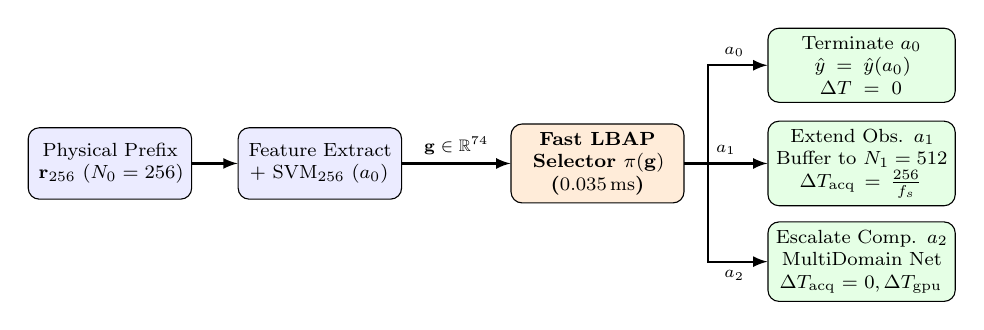
\begin{tikzpicture}[scale=0.86, every node/.style={transform shape}]
    % Styles
    \tikzset{
        block/.style={rectangle, draw, fill=blue!8, text width=6.2em, text centered, rounded corners, minimum height=3.0em, font=\footnotesize},
        gate/.style={rectangle, draw, fill=orange!15, text width=6.6em, text centered, rounded corners, minimum height=3.2em, font=\footnotesize\bfseries},
        action/.style={rectangle, draw, fill=green!10, text width=7.2em, text centered, rounded corners, minimum height=3.0em, font=\footnotesize},
        line/.style={draw, -latex, thick}
    }

    % Nodes with wide explicit coordinates to prevent arrow/label collisions
    \node [block] (input) at (0, 0) {Physical Prefix\\$\mathbf{r}_{256}$ ($N_0=256$)};
    \node [block] (base) at (3.1, 0) {Feature Extract\\+ $\mathrm{SVM}_{256}$ ($a_0$)};
    \node [gate] (lbap) at (7.2, 0) {Fast LBAP\\Selector $\pi(\mathbf{g})$\\($0.035\,\mathrm{ms}$)};
    
    \node [action] (act0) at (11.1, 1.45) {Terminate $a_0$\\$\hat{y} = \hat{y}(a_0)$\\$\Delta T = 0$};
    \node [action] (act1) at (11.1, 0.0) {Extend Obs. $a_1$\\Buffer to $N_1=512$\\$\Delta T_{\mathrm{acq}} = \frac{256}{f_s}$};
    \node [action] (act2) at (11.1, -1.45) {Escalate Comp. $a_2$\\MultiDomain Net\\$\Delta T_{\mathrm{acq}} = 0, \Delta T_{\mathrm{gpu}}$};

    % Paths
    \path [line] (input) -- (base);
    \path [line] (base) -- node[above, font=\scriptsize] {$\mathbf{g}\in\mathbb{R}^{74}$} (lbap);
    \path [line] (lbap.east) -- ++(0.35, 0) |- node[pos=0.72, above, font=\scriptsize] {$a_0$} (act0.west);
    \path [line] (lbap.east) -- node[above, font=\scriptsize] {$a_1$} (act1.west);
    \path [line] (lbap.east) -- ++(0.35, 0) |- node[pos=0.72, below, font=\scriptsize] {$a_2$} (act2.west);
\end{tikzpicture}%
}
\caption{Sequential execution pipeline of the proposed joint observation-computation policy. The gating decision $\pi(\mathbf{g})$ is reached in $<0.05\,\mathrm{ms}$ from prefix observables, branching into immediate termination ($a_0$), physical window extension ($a_1$), or GPU multi-domain neural escalation ($a_2$).}
\label{fig:pipeline_flowchart}
\end{figure}

\begin{table}[t]
\caption{Operational Characteristics of the Tripartite Action Set $\mathcal{A}$ (Full-Route Synced Profiling, 3 Sessions $\times$ 300 Calls)}
\label{tab:action_characteristics}
\centering
\renewcommand{\arraystretch}{1.2}
\setlength{\tabcolsep}{4.5pt}
\resizebox{\columnwidth}{!}{%
\begin{tabular}{lccccc}
\hline
\textbf{Action} & \textbf{Model} & \textbf{Horizon} & $T_{\mathrm{acq}}$ ($f_s=8\mathrm{k}$) & $T_{\mathrm{comp}}$ (Batch=1, Sync) & \textbf{Dominant Resilience} \\
\hline
$a_0$ & $\mathrm{SVM}_{256}$ & $N_0 = 256$ & $32.00\,\mathrm{ms}$ & $2.22\,\mathrm{ms}$ (CPU) & High SNR, benign AWGN \\
$a_1$ & $\mathrm{SVM}_{512}$ & $N_1 = 512$ & $64.00\,\mathrm{ms}$ & $3.22\,\mathrm{ms}$ (CPU) & Finite-sample moment jitter \\
$a_2$ & MultiDomain & $N_0 = 256$ & $32.00\,\mathrm{ms}$ & $32.55\,\mathrm{ms}$ (GPU) & Mid-SNR, CFO, multipath, ISI \\
\hline
\end{tabular}%
}
\end{table}

\textbf{Zero-Leakage Invariance Guarantee:} Under this protocol, the policy vector $\mathbf{g}(\mathbf{r}_{256})$ contains strictly causal, observable indicators extracted from $\mathbf{r}_{256}$ and the uncalibrated decision hyperplane projections of $\mathrm{SVM}_{256}$. At no point does the selector access oracle signal-to-noise ratio ($\mathrm{SNR}_{\mathrm{true}}$), ground-truth carrier frequency offset ($\mathrm{CFO}_{\mathrm{true}}$), propagation taps, unbuffered samples $r[256:512]$, or counterfactual predictions from models not yet executed.

% -------------------------------------------------------------------------
\subsection{Strict Latency Decomposition and Sequential Cost Modeling}
\label{subsec:latency_decomposition}

A rigorous deployment model requires separating physical sampling delays from algorithmic computation, while accounting for the sequential dependencies of routed inference. The total wall-clock reception latency for action $a \in \mathcal{A}$ is given by:
\begin{equation}
    T_{\mathrm{total}}(a) = T_{\mathrm{acq}}(a) + T_{\mathrm{comp}}(a),
    \label{eq:t_total_general}
\end{equation}
where the virtual physical acquisition latency is defined strictly by the ADC sampling clock:
\begin{equation}
    T_{\mathrm{acq}}(a) = \frac{N(a)}{f_s}.
    \label{eq:t_acq}
\end{equation}
For $N_0 = 256$ and $f_s = 8000\,\mathrm{Hz}$, $T_{\mathrm{acq}}(a_0) = T_{\mathrm{acq}}(a_2) = 32.0\,\mathrm{ms}$. For $N_1 = 512$, $T_{\mathrm{acq}}(a_1) = 64.0\,\mathrm{ms}$, enforcing a penalty of $\Delta T_{\mathrm{acq}} = 32.0\,\mathrm{ms}$.

In real-time firmware, computing the gating vector $\mathbf{g}$ requires first extracting features from the prefix $\mathbf{r}_{256}$ and evaluating the baseline classifier $a_0$. Denoting the baseline execution latency by $T_{\mathrm{base}, 0}$ and the Fast LBAP evaluation latency by $T_{\mathrm{gate}}$, the sequential computational cost $T_{\mathrm{comp}}(a)$ under routed execution is non-separable:
\begin{align}
    T_{\mathrm{comp}}(a_0) &= T_{\mathrm{base}, 0} + T_{\mathrm{gate}}, \label{eq:t_comp_a0} \\
    T_{\mathrm{comp}}(a_1) &= T_{\mathrm{base}, 0} + T_{\mathrm{gate}} + T_{\mathrm{base}, 1}, \label{eq:t_comp_a1} \\
    T_{\mathrm{comp}}(a_2) &= T_{\mathrm{base}, 0} + T_{\mathrm{gate}} + T_{\mathrm{base}, 2}, \label{eq:t_comp_a2}
\end{align}
where $T_{\mathrm{base}, 1}$ represents the feature extraction and classification time of $\mathrm{SVM}_{512}$, and $T_{\mathrm{base}, 2}$ is the forward-pass execution time of $\mathrm{MultiDomainAMCNet}$.

\textbf{Measurement Protocol (N3.3 Full-Route Synchronization):} Computation latencies are profiled in true single-sample streaming mode ($\text{batch}=1$) under explicit CUDA synchronization ($\mathtt{torch.cuda.synchronize()}$) and single-thread contention controls ($\mathtt{torch.set\_num\_threads(1)}$, $\mathtt{threadpool\_limits(limits=1)}$) across three randomized sessions of $300$ independent waveforms ($900$ measured calls per policy). Unlike unrouted kernel timings ($2.03\text{--}24.15\,\mathrm{ms}$ in preliminary profiling), full-route execution includes the prefix extractor and selector overhead whenever routing occurs: standalone baselines average $T_{\mathrm{base}, 0} = 2.221\,\mathrm{ms}$ ($\mathrm{SVM}_{256}$), $T_{\mathrm{base}, 1} = 3.218\,\mathrm{ms}$ ($\mathrm{SVM}_{512}$), and $T_{\mathrm{base}, 2} = 32.545\,\mathrm{ms}$ ($\mathrm{MultiDomainAMCNet}$ on RTX 4060 Laptop GPU, median $28.29\,\mathrm{ms}$, P95 $58.25\,\mathrm{ms}$). Under full-route conditional branching, routed Fast LBAP compute averages $18.688\,\mathrm{ms}$ overall (median $6.555\,\mathrm{ms}$, P95 $46.639\,\mathrm{ms}$), cutting compute time by $13.857\,\mathrm{ms}$ vs.\ standalone $a_2$ ($95\%$ CI $[-15.348, -12.317]\,\mathrm{ms}$), with realized per-branch compute costs of $4.133\,\mathrm{ms}$ ($a_0$ exit), $6.621\,\mathrm{ms}$ ($a_1$ exit), and $36.763\,\mathrm{ms}$ ($a_2$ exit).

% -------------------------------------------------------------------------
\subsection{Net Utility Formulation: Recoverability vs. Irrecuperability}
\label{subsec:net_utility}

Let $y \in \mathcal{C} = \{\mathrm{BPSK}, \mathrm{QPSK}, \mathrm{8PSK}, \allowbreak \mathrm{16QAM}, \mathrm{64QAM}, \mathrm{4PAM}\}$ denote the modulation class, and $\hat{y}(a)$ the discrete prediction emitted by action $a \in \mathcal{A}$. The binary classification success indicator is defined as $I(a; \mathbf{r}, y) = \mathbb{I}(\hat{y}(a) = y) \in \{0, 1\}$.

We define the scalar \emph{net engineering utility} $U(a; \mathbf{r}, y)$ by penalizing incorrect classifications while amortizing total reception latency via a latency-cost trade-off coefficient $\lambda \ge 0$ ($\mathrm{ms}^{-1}$):
\begin{equation}
    U(a; \mathbf{r}, y) = \mathbb{I}(\hat{y}(a) = y) - \lambda \, T_{\mathrm{total}}(a).
    \label{eq:net_utility_def}
\end{equation}
The optimal Bayes policy $\pi^*$ maps the observable gating vector $\mathbf{g} \in \mathcal{G}$ to the action that maximizes the conditional expected net utility:
\begin{align}
    \pi^*(\mathbf{g}) &= \arg\max_{a \in \mathcal{A}} \; \mathbb{E}_{y, \mathbf{r} \mid \mathbf{g}} \left[ U(a; \mathbf{r}, y) \right] \nonumber \\
    &= \arg\max_{a \in \mathcal{A}} \; \left\{ \mathbb{P}(\hat{y}(a) = y \mid \mathbf{g}) - \lambda \, T_{\mathrm{total}}(a) \right\}.
    \label{eq:bayes_optimal_policy}
\end{align}

\subsubsection{The Failure of Confidence-Threshold Early Exiting}
Conventional early-exit AMC architectures \cite{liu2026beacon, liu2025joint} rely on max-softmax probability or classification margin:
\begin{equation}
    \pi_{\mathrm{conf}}(\mathbf{g}) = \begin{cases} a_0, & \text{if } \hat{P}(\hat{y}(a_0) = y \mid \mathbf{g}) \ge \tau_{\mathrm{conf}}, \\ a_k, & \text{otherwise}, \end{cases}
    \label{eq:conf_policy}
\end{equation}
where $a_k \in \{a_1, a_2\}$ is a designated complex branch. However, conditioning solely on early confidence fails to maximize net utility due to the fundamental asymmetry between four mutually exclusive sample regimes (illustrated in Fig.~\ref{fig:recoverability_quadrants}):

\begin{figure}[t]
\centering
\resizebox{\columnwidth}{!}{%
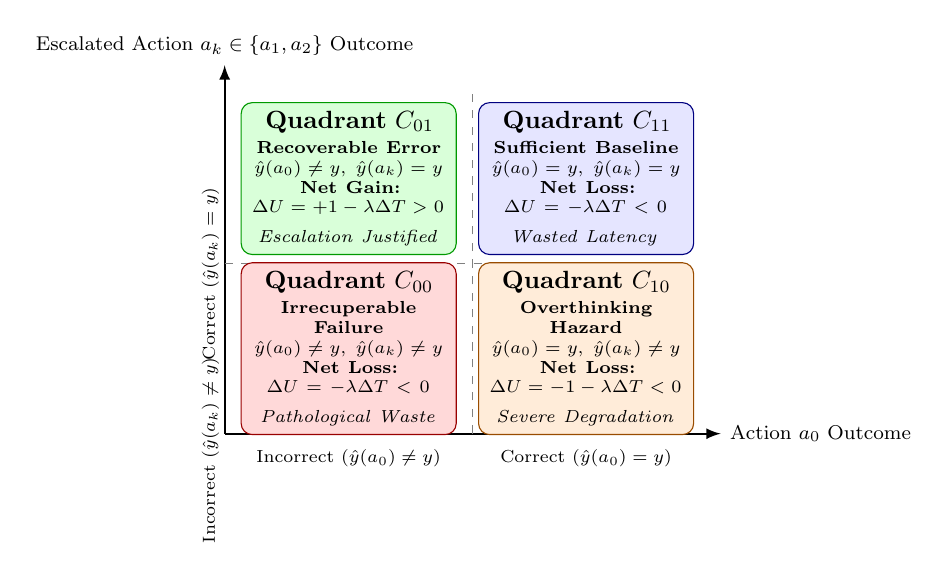
\begin{tikzpicture}[scale=0.9, every node/.style={transform shape}]
    % Grid
    \draw[thick, -latex] (0,0) -- (7,0) node[right, font=\footnotesize] {Action $a_0$ Outcome};
    \draw[thick, -latex] (0,0) -- (0,5.2) node[above, font=\footnotesize] {Escalated Action $a_k \in \{a_1, a_2\}$ Outcome};
    
    % Dividing lines
    \draw[dashed, gray] (3.5,0) -- (3.5,4.8);
    \draw[dashed, gray] (0,2.4) -- (6.5,2.4);
    
    % Quadrants
    % Top Left: C01 Recoverable
    \node[fill=green!15, rounded corners, draw=green!60!black, text width=2.8cm, text centered, minimum height=1.9cm] at (1.75, 3.6) {
        \textbf{Quadrant $C_{01}$}\\[2pt]
        \scriptsize \textbf{Recoverable Error}\\
        $\hat{y}(a_0) \neq y, \; \hat{y}(a_k) = y$\\
        \textbf{Net Gain:}\\
        $\Delta U = +1 - \lambda \Delta T > 0$\\
        \emph{Escalation Justified}
    };
    
    % Top Right: C11 Both Correct
    \node[fill=blue!10, rounded corners, draw=blue!50!black, text width=2.8cm, text centered, minimum height=1.9cm] at (5.1, 3.6) {
        \textbf{Quadrant $C_{11}$}\\[2pt]
        \scriptsize \textbf{Sufficient Baseline}\\
        $\hat{y}(a_0) = y, \; \hat{y}(a_k) = y$\\
        \textbf{Net Loss:}\\
        $\Delta U = -\lambda \Delta T < 0$\\
        \emph{Wasted Latency}
    };
    
    % Bottom Left: C00 Irrecuperable
    \node[fill=red!15, rounded corners, draw=red!60!black, text width=2.8cm, text centered, minimum height=1.9cm] at (1.75, 1.2) {
        \textbf{Quadrant $C_{00}$}\\[2pt]
        \scriptsize \textbf{Irrecuperable Failure}\\
        $\hat{y}(a_0) \neq y, \; \hat{y}(a_k) \neq y$\\
        \textbf{Net Loss:}\\
        $\Delta U = -\lambda \Delta T < 0$\\
        \emph{Pathological Waste}
    };
    
    % Bottom Right: C10 Overthinking
    \node[fill=orange!15, rounded corners, draw=orange!60!black, text width=2.8cm, text centered, minimum height=1.9cm] at (5.1, 1.2) {
        \textbf{Quadrant $C_{10}$}\\[2pt]
        \scriptsize \textbf{Overthinking Hazard}\\
        $\hat{y}(a_0) = y, \; \hat{y}(a_k) \neq y$\\
        \textbf{Net Loss:}\\
        $\Delta U = -1 - \lambda \Delta T < 0$\\
        \emph{Severe Degradation}
    };
    
    % Labels on axes
    \node[below, font=\scriptsize] at (1.75, -0.1) {Incorrect ($\hat{y}(a_0) \neq y$)};
    \node[below, font=\scriptsize] at (5.1, -0.1) {Correct ($\hat{y}(a_0) = y$)};
    \node[left, font=\scriptsize, rotate=90] at (-0.2, 1.2) {Incorrect ($\hat{y}(a_k) \neq y$)};
    \node[left, font=\scriptsize, rotate=90] at (-0.2, 3.6) {Correct ($\hat{y}(a_k) = y$)};
\end{tikzpicture}%
}
\caption{Taxonomy of joint classification events between baseline $a_0$ and complex action $a_k \in \{a_1, a_2\}$. Escalate decisions are profitable \emph{only} in Quadrant $C_{01}$ (recoverable errors). Confidence thresholds cannot distinguish $C_{01}$ from $C_{00}$, squandering budget in deep-noise regimes.}
\label{fig:recoverability_quadrants}
\end{figure}

\begin{itemize}
    \item \textbf{Quadrant $C_{11}$ (Both Correct):} Both $a_0$ and $a_k$ yield the correct class. Escalating to $a_k$ yields zero accuracy improvement while incurring latency penalty $\Delta T = T_{\mathrm{total}}(a_k) - T_{\mathrm{total}}(a_0)$, resulting in a net utility loss $\Delta U = -\lambda \Delta T < 0$.
    
    \item \textbf{Quadrant $C_{01}$ (Recoverable Error):} Baseline $a_0$ fails ($\hat{y}(a_0) \neq y$) but $a_k$ succeeds ($\hat{y}(a_k) = y$). Escalation recovers the correct class, generating a net gain $\Delta U = +1 - \lambda \Delta T > 0$ provided $\lambda \Delta T < 1$.
    
    \item \textbf{Quadrant $C_{00}$ (Irrecuperable Error):} Both $a_0$ and $a_k$ fail due to extreme channel degradation (e.g., $\mathrm{SNR} \le -15\,\mathrm{dB}$ or deep spectral nulls below the Shannon classification limit). Escalation produces no accuracy improvement and incurs full latency penalty: $\Delta U = -\lambda \Delta T < 0$.
    
    \item \textbf{Quadrant $C_{10}$ (Overthinking / Degradation):} Baseline $a_0$ succeeds, but $a_k$ misclassifies due to representation sensitivity or overfitting. Escalation incurs a catastrophic penalty $\Delta U = -1 - \lambda \Delta T \ll 0$.
\end{itemize}

Under severe noise ($C_{00}$), classifier $a_0$ exhibits near-zero margin and maximal entropy, exactly mirroring its behavior on recoverable edge cases ($C_{01}$). Consequently, any scalar threshold $\tau_{\mathrm{conf}}$ triggers escalation on both $C_{01}$ and $C_{00}$, expending massive acquisition and compute budgets on hopelessly corrupted signals. In contrast, maximizing expected net utility \eqref{eq:bayes_optimal_policy} directly estimates the counterfactual recovery probability:
\begin{align}
    \Delta \hat{U}_{k \mid 0}(\mathbf{g}) &= \hat{\mathbb{P}}(C_{01}^{(k)} \mid \mathbf{g}) - \hat{\mathbb{P}}(C_{10}^{(k)} \mid \mathbf{g}) \nonumber \\
    &\quad - \lambda [T_{\mathrm{total}}(a_k) - T_{\mathrm{total}}(a_0)],
    \label{eq:delta_utility}
\end{align}
which is positive \emph{if and only if} the likelihood of recovery exceeds the cost-adjusted risk of unrecoverable or degraded execution.

\subsubsection{Physical Bifurcation of Recoverable Errors}
Furthermore, the proposed tripartite action space admits a physical bifurcation of recoverable errors:
\begin{equation}
    C_{01} = C_{01}^{(a_1)} \cup C_{01}^{(a_2)}.
    \label{eq:bifurcation}
\end{equation}
When distortion arises from finite-sample moment estimation variance in stationary moderate-SNR channels, high-order statistics stabilize over longer durations; such errors belong to $C_{01}^{(a_1)}$ and are resolved by extending observation to $N_1 = 512$ ($a_1$). Conversely, when errors are caused by multipath frequency selectivity, residual carrier offset, or high-order constellation crowding ($16\mathrm{QAM} / 64\mathrm{QAM}$), expanding $N$ with scalar moment classifiers provides negligible gain. Such errors belong to $C_{01}^{(a_2)}$ and require the polyphase attention and multi-harmonic spectral transformations of $a_2$. The policy must therefore discern not merely whether to escalate, but \emph{which physical resource} (observation vs. computation) recovers the transmission.

% -------------------------------------------------------------------------
\subsection{Fast LBAP Selector Architecture and Formulation}
\label{subsec:lbap_architecture}

To evaluate \eqref{eq:bayes_optimal_policy} within real-time budgets ($<0.05\,\mathrm{ms}$), we design the \emph{Fast LBAP Selector} as a hybrid architecture coupling a convex Ridge regularizer with an ultra-compact two-layer Multi-Layer Perceptron (MLP), implemented in vectorized C-contiguous NumPy array routines.

\subsubsection{Gating Representation Vector $\mathbf{g} \in \mathbb{R}^{74}$}
The gating vector $\mathbf{g} = [\mathbf{f}_{256}^T, \mathbf{s}^T, m, \hat{p}_0, H]^T \in \mathbb{R}^{74}$ encapsulates:
\begin{enumerate}
    \item \textbf{Statistical and Spectral Features ($\mathbf{f}_{256} \in \mathbb{R}^{65}$):} Sample cumulants ($\hat{C}_{20}, \hat{C}_{40}, \hat{C}_{42}, \hat{C}_{60}, \hat{C}_{63}$), normalized envelope central moments up to 6th order, cyclic phase projections $R_k = |\mathbb{E}[e^{j k \arg(r[n])}]|$ for $k \in \{1, 2, 4, 8\}$, spectral flatness, and spectral entropy.
    \item \textbf{SVM Decision Projections ($\mathbf{s} \in \mathbb{R}^6$):} The signed uncalibrated distances $s_c(\mathbf{f}_{256})$ to the decision hyperplanes for all six classes $c \in \mathcal{C}$ generated by $\mathrm{SVM}_{256}$.
    \item \textbf{Top-Two Margin ($m \in \mathbb{R}$):} The difference between the highest and second-highest decision scores: $m = s_{(1)} - s_{(2)} \ge 0$.
    \item \textbf{Calibrated Posterior Confidence ($\hat{p}_0 \in [0, 1]$):} The logistic-calibrated probability of baseline correctness $\hat{p}_0 = \sigma(\beta_1 m + \beta_0)$ fitted strictly on validation data (Section~\ref{subsec:calibration}).
    \item \textbf{Normalized Decision Entropy ($H \in [0, 1]$):} Evaluating ambiguity across the class distribution:
    \begin{equation}
        H = -\frac{1}{\ln 6} \sum_{c=1}^6 \tilde{p}_c \ln(\tilde{p}_c + \epsilon), \quad \tilde{\mathbf{p}} = \mathrm{softmax}(\mathbf{s}).
        \label{eq:decision_entropy}
    \end{equation}
\end{enumerate}

\subsubsection{Hybrid Ridge--MLP Estimator}
Input features are standardized using frozen parameters computed on the training set:
\begin{equation}
    \tilde{\mathbf{g}} = \mathrm{clip}\left( \frac{\mathbf{g} - \boldsymbol{\mu}_{\mathbf{g}}}{\boldsymbol{\sigma}_{\mathbf{g}} + \epsilon_{\mathrm{scale}}}, -10.0, 10.0 \right) \in \mathbb{R}^{74}.
    \label{eq:input_standardization}
\end{equation}

The utility predictor decomposes into two complementary functional pathways:
\begin{enumerate}
    \item \textbf{Linear Ridge Pathway (Global Regularized Baseline):}
    \begin{equation}
        \mathbf{u}_{\mathrm{lin}}(\mathbf{g}) = \tilde{\mathbf{g}} \mathbf{W}_{\mathrm{lin}} + \mathbf{b}_{\mathrm{lin}},
        \label{eq:ridge_path}
    \end{equation}
    where $\mathbf{W}_{\mathrm{lin}} \in \mathbb{R}^{74 \times 3}$ and $\mathbf{b}_{\mathrm{lin}} \in \mathbb{R}^3$ are solved in closed form via Tikhonov regularization with parameter $\gamma_{\mathrm{ridge}} = 40.0$:
    \begin{equation}
        \mathbf{W}_{\mathrm{lin}} = (\tilde{\mathbf{G}}^T \tilde{\mathbf{G}} + \gamma_{\mathrm{ridge}} \mathbf{I})^{-1} \tilde{\mathbf{G}}^T (\mathbf{Y}_{\mathrm{util}} - \bar{\mathbf{Y}}_{\mathrm{util}}),
        \label{eq:ridge_closed_form}
    \end{equation}
    guaranteeing bounded variance and numerical stability across collinear cumulant features.
    
    \item \textbf{Non-Linear MLP Pathway (Local Interaction Modeler):}
    \begin{align}
        \mathbf{h} &= \max(0, \tilde{\mathbf{g}} \mathbf{W}_1 + \mathbf{b}_1), \quad \mathbf{h} \in \mathbb{R}^{d_h}, \label{eq:mlp_hidden} \\
        \mathbf{u}_{\mathrm{mlp}}(\mathbf{g}) &= \mathbf{h} \mathbf{W}_2 + \mathbf{b}_2, \quad \mathbf{u}_{\mathrm{mlp}} \in \mathbb{R}^3, \label{eq:mlp_output}
    \end{align}
    with hidden dimension $d_h = 64$. The MLP parameters are trained to minimize the robust Huber (Smooth $L_1$) loss against ground-truth counterfactual utilities:
    \begin{equation}
        \mathcal{L}_{\mathrm{Huber}}(\mathbf{u}, \mathbf{y}) = \sum_{a=0}^2 \begin{cases} 
            0.5 (u_a - y_a)^2, & |u_a - y_a| \le 1, \\
            |u_a - y_a| - 0.5, & \text{otherwise},
        \end{cases}
        \label{eq:huber_loss}
    \end{equation}
    optimized via AdamW (learning rate $\eta = 3\times 10^{-3}$, weight decay $10^{-3}$, $400$ epochs).
\end{enumerate}

\subsubsection{Convex Ensembling and Action Selection}
The final predicted utility vector $\hat{\mathbf{u}}(\mathbf{g}) = [\hat{u}_0, \hat{u}_1, \hat{u}_2]^T$ blends both pathways:
\begin{equation}
    \hat{\mathbf{u}}(\mathbf{g}) = \alpha^* \mathbf{u}_{\mathrm{mlp}}(\mathbf{g}) + (1 - \alpha^*) \mathbf{u}_{\mathrm{lin}}(\mathbf{g}),
    \label{eq:blended_utility}
\end{equation}
where the ensembling weight $\alpha^* \in \{0.0, 0.25, 0.50, 0.75, 1.0\}$ is tuned on an independent validation set $\mathcal{V}_{\mathrm{select}}$ to maximize realized classification utility. The policy selects the action that maximizes predicted net utility over the allowed action subset $\mathcal{A}_{\mathrm{allowed}} \subseteq \mathcal{A}$:
\begin{equation}
    a^*(\mathbf{g}) = \arg\max_{a \in \mathcal{A}_{\mathrm{allowed}}} \; \hat{u}_a(\mathbf{g}).
    \label{eq:final_action_choice}
\end{equation}

When restricted to $\mathcal{A}_{\mathrm{allowed}} = \{a_0, a_1\}$, the model reduces to pure adaptive acquisition (Fewer-Sample style); when restricted to $\mathcal{A}_{\mathrm{allowed}} = \{a_0, a_2\}$, it instantiates early-exit computational escalation (BEACON style). The unrestricted set $\mathcal{A}_{\mathrm{allowed}} = \{a_0, a_1, a_2\}$ realizes joint observation-computation optimization.

% -------------------------------------------------------------------------
\subsection{Rigorous Probabilistic Calibration and Temperature Scaling}
\label{subsec:calibration}

In safety-critical wireless systems, decision policies must not rely on uncalibrated heuristic scores. Raw margin scores from SVMs and uncalibrated softmax logits from deep neural networks suffer from severe overconfidence in low-SNR and out-of-distribution (OOD) regimes \cite{yang2026uncertainty}. To prevent policy distortion, we establish rigorous calibration protocols on an isolated calibration partition $\mathcal{V}_{\mathrm{cal}}$ ($1200$ balanced signals) strictly disjoint from both the policy-selection partition $\mathcal{V}_{\mathrm{select}}$ ($1200$ signals) and the test splits.

\subsubsection{Margin-Based Platt Calibration for Baseline $a_0$}
For $\mathrm{SVM}_{256}$, class assignment is determined by $\hat{y}(a_0) = \arg\max_{c \in \mathcal{C}} s_c$. The probability that this assignment is correct is modeled via a univariate logistic sigmoid over the margin $m = s_{(1)} - s_{(2)}$:
\begin{equation}
    \hat{P}(Y = \hat{y}(a_0) \mid m) = \sigma(\beta_1 m + \beta_0) = \frac{1}{1 + e^{-(\beta_1 m + \beta_0)}},
    \label{eq:platt_margin}
\end{equation}
where parameters $\boldsymbol{\beta} = [\beta_1, \beta_0]^T$ are fitted by minimizing the binary cross-entropy loss over $\mathcal{V}_{\mathrm{cal}}$ with $L_2$ regularization:
\begin{align}
    \min_{\boldsymbol{\beta}} \; -\sum_{i \in \mathcal{V}_{\mathrm{cal}}} \Big[ &z_i \ln \sigma(\beta_1 m_i + \beta_0) \nonumber \\
    &+ (1 - z_i) \ln\big(1 - \sigma(\beta_1 m_i + \beta_0)\big) \Big],
    \label{eq:logistic_cal_loss}
\end{align}
where $z_i = \mathbb{I}(\hat{y}^{(i)}(a_0) = y^{(i)})$. This single calibrated probability $\hat{p}_0$ is injected directly into dimension $73$ of the gating vector $\mathbf{g}$.

\subsubsection{Temperature Scaling for Deep Expert $a_2$}
For $\mathrm{MultiDomainAMCNet}$ ($a_2$), raw forward inference outputs unnormalized logits $\mathbf{z}(\mathbf{r}_{256}) \in \mathbb{R}^6$. Applying a naive softmax $p_k = e^{z_k} / \sum_j e^{z_j}$ produces miscalibrated confidence scores under channel mismatch. We apply parametric Temperature Scaling \cite{yang2026uncertainty}, modifying logits by a single strictly positive scalar temperature $T > 0$:
\begin{equation}
    \hat{p}_k(\mathbf{r}_{256}; T) = \frac{\exp(z_k / T)}{\sum_{j=1}^6 \exp(z_j / T)}, \quad \forall k \in \{1, \dots, 6\}.
    \label{eq:temp_scaling}
\end{equation}
The optimal temperature $T^*$ is identified by minimizing the multiclass Negative Log-Likelihood (NLL) over the held-out calibration set $\mathcal{V}_{\mathrm{cal}}$:
\begin{equation}
    T^* = \arg\min_{T > 0} \; -\sum_{i \in \mathcal{V}_{\mathrm{cal}}} \sum_{c=1}^6 \mathbb{I}(y^{(i)} = c) \ln \hat{p}_c(\mathbf{r}_{256}^{(i)}; T),
    \label{eq:temp_nll_opt}
\end{equation}
solved via the quasi-Newton L-BFGS optimizer. Crucially, because the transformation $\mathbf{z} / T$ is strictly monotonic for any $T > 0$, temperature scaling preserves the classification output $\arg\max_k z_k$ and the top-1 accuracy identically, while calibrating the output probabilities to align with empirical accuracy.

Calibration quality for top-1 confidence reliability is quantified via the Expected Calibration Error ($\mathrm{ECE}_{10}$) over $K=10$ uniform equal-width bins in $[0, 1]$:
\begin{equation}
    \mathrm{ECE}_{10} = \sum_{b=1}^{10} \frac{|B_b|}{N_{\mathrm{val}}} \left| \mathrm{acc}(B_b) - \mathrm{conf}(B_b) \right|,
    \label{eq:ece_def}
\end{equation}
together with binary top-1 correctness Brier score $\mathrm{BS}_{\mathrm{bin}} = \frac{1}{N} \sum_{i=1}^N (\hat{p}_{i,\max} - z_i)^2$ and binary Negative Log-Likelihood $\mathrm{NLL}_{\mathrm{bin}} = -\frac{1}{N}\sum_{i=1}^N [z_i \ln \hat{p}_{i,\max} + (1 - z_i)\ln(1 - \hat{p}_{i,\max})]$, where $z_i = \mathbb{I}(\hat{y}_i = y_i)$ and $\hat{p}_{i,\max} = \max_c \hat{p}_{ic}$ (allowing unified scalar reliability comparison across both the binary Platt margin of $a_0$ and the maximum calibrated probability of $a_2$). Note that $T^*$ is nevertheless optimized via multiclass NLL~\eqref{eq:temp_nll_opt}. As quantified in Section~\ref{sec:results_discussion}, post-hoc calibration aligns the in-distribution confidence scores of both the baseline SVM and the deep expert with empirical accuracy, while revealing overconfidence degradation under severe OOD shift.

% -------------------------------------------------------------------------
\subsection{Pareto Optimality across Latency Regimes and Sampling Frequencies}
\label{subsec:pareto_formulation}

A fundamental advantage of the proposed net utility formulation is its adaptability across heterogeneous operational environments. By varying the latency cost parameter $\lambda$ and analyzing system behavior across different front-end ADC sampling frequencies $f_s$, the Fast LBAP selector defines an optimal Pareto frontier balancing classification risk $R(\pi) = 1 - \mathrm{Acc}(\pi)$ against total reception latency $T_{\mathrm{total}}(\pi)$.

\begin{figure}[t]
\centering
\resizebox{\columnwidth}{!}{%
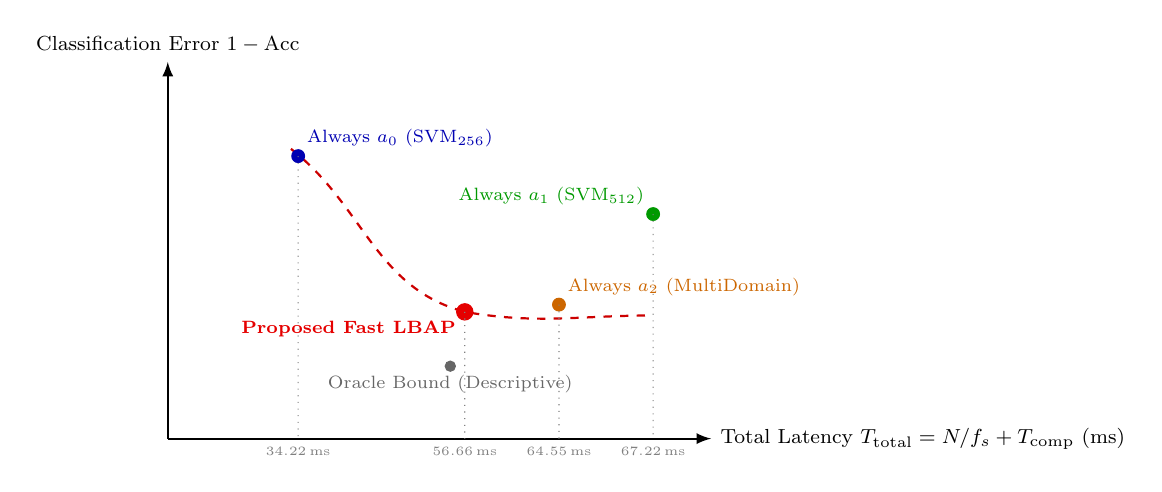
\begin{tikzpicture}[scale=0.92, every node/.style={transform shape}]
    % Axes
    \draw[thick, -latex] (0,0) -- (7.5,0) node[right, font=\footnotesize] {Total Latency $T_{\mathrm{total}} = N/f_s + T_{\mathrm{comp}}$ (ms)};
    \draw[thick, -latex] (0,0) -- (0,5.2) node[above, font=\footnotesize] {Classification Error $1 - \mathrm{Acc}$};

    % Baselines
    \coordinate (A0) at (1.8, 3.9);
    \coordinate (A1) at (6.7, 3.1);
    \coordinate (A2) at (5.4, 1.85);
    \coordinate (LBAP_opt) at (4.1, 1.75);
    \coordinate (Oracle) at (3.9, 1.0);

    % Pareto curve
    \draw[dashed, red!80!black, thick] (1.7, 4.0) to[out=-38, in=165] (4.1, 1.75) to[out=-10, in=180] (6.7, 1.7);

    % Points
    \filldraw[blue!70!black] (A0) circle (2.5pt) node[above right, font=\scriptsize] {Always $a_0$ ($\mathrm{SVM}_{256}$)};
    \filldraw[green!60!black] (A1) circle (2.5pt) node[above left, font=\scriptsize] {Always $a_1$ ($\mathrm{SVM}_{512}$)};
    \filldraw[orange!80!black] (A2) circle (2.5pt) node[above right, font=\scriptsize] {Always $a_2$ (MultiDomain)};
    \filldraw[red!90!black] (LBAP_opt) circle (3.2pt) node[below left, font=\scriptsize\bfseries] {Proposed Fast LBAP};
    \filldraw[gray!80!black] (Oracle) circle (2pt) node[below, font=\scriptsize] {Oracle Bound (Descriptive)};

    % Grid lines
    \draw[dotted, gray] (A0) -- (1.8,0) node[below, font=\tiny] {$34.22\,\mathrm{ms}$};
    \draw[dotted, gray] (LBAP_opt) -- (4.1,0) node[below, font=\tiny] {$56.66\,\mathrm{ms}$};
    \draw[dotted, gray] (A2) -- (5.4,0) node[below, font=\tiny] {$64.55\,\mathrm{ms}$};
    \draw[dotted, gray] (A1) -- (6.7,0) node[below, font=\tiny] {$67.22\,\mathrm{ms}$};
\end{tikzpicture}%
}
\caption{Conceptual Risk--Latency Pareto frontier at $f_s = 8\,\mathrm{kHz}$ using synced full-route latency profiling (\texttt{N3.3}). At low sampling rates, the physical waiting penalty of $a_1$ ($+32\,\mathrm{ms}$) makes standalone $a_1$ ($67.22\,\mathrm{ms}$) slower than standalone $a_2$ ($64.55\,\mathrm{ms}$); deployable Fast LBAP routes across $\{a_0,a_1,a_2\}$ to achieve lower mean latency ($56.66\,\mathrm{ms}$) and higher utility ($0.4379$) than standalone $a_2$ ($0.4190$).}
\label{fig:pareto_conceptual}
\end{figure}

\subsubsection{Parametric Sensitivity to Trade-Off Coefficient $\lambda$}
The parameter $\lambda \ge 0$ represents the exchange rate between classification accuracy and reception delay:
\begin{itemize}
    \item \textbf{Accuracy-Centric Regime ($\lambda \to 0$):} Latency is unpenalized. The policy collapses to an accuracy oracle, selecting $\arg\max_{a \in \mathcal{A}} \mathbb{P}(\hat{y}(a) = y \mid \mathbf{g})$. Difficult frames are routed aggressively to the most accurate models ($a_2$ or $a_1$).
    \item \textbf{Latency-Constrained Regime ($\lambda \ge 0.005\,\mathrm{ms}^{-1}$):} An additional $32\,\mathrm{ms}$ acquisition delay penalizes net utility by $\Delta U = -0.160$. Under high latency pressure, the policy restricts escalation to high-recoverability prefixes and shifts substantially back toward immediate $a_0$ termination.
    \item \textbf{Balanced Operational Regime ($\lambda = 0.0015\,\mathrm{ms}^{-1}$):} Our nominal operating point values $10\,\mathrm{ms}$ of reception delay at $0.015$ accuracy points ($32\,\mathrm{ms}$ at $0.048$ points), balancing neural recovery against both acquisition wait ($a_1$) and single-sample inference time ($a_2$). Under this nominal trade-off with full-route synced costs, Fast LBAP improves net utility over all fixed standalone baselines in-distribution while remaining faster on average than either standalone $a_1$ or standalone $a_2$.
\end{itemize}

\subsubsection{Asymptotic Inversion with Sampling Rate $f_s$}
The relative economic advantage between action $a_1$ (more observation) and action $a_2$ (more computation) is an explicit function of the ADC sampling rate $f_s$:
\begin{align}
    \lim_{f_s \to \infty} T_{\mathrm{acq}}(a) &= 0, \quad \forall a \in \mathcal{A}, \label{eq:limit_fs_inf} \\
    \lim_{f_s \to 0} \frac{T_{\mathrm{acq}}(a_1)}{T_{\mathrm{comp}}(a_2)} &= \infty. \label{eq:limit_fs_zero}
\end{align}

In low-rate sensor and IoT networks ($f_s \approx 8\,\mathrm{kHz}$, symbol rate $R_s = 1000\,\mathrm{Bd}$), physical acquisition dominates: waiting for $256$ additional samples adds $T_{\mathrm{acq}}(a_1) - T_{\mathrm{acq}}(a_0) = 32.0\,\mathrm{ms}$ ($67.22\,\mathrm{ms}$ synced total for standalone $a_1$), whereas deep neural inference requires $T_{\mathrm{base}, 2} = 32.55\,\mathrm{ms}$ ($64.55\,\mathrm{ms}$ synced total for standalone $a_2$). In this narrowband regime, computational escalation ($a_2$) on the short $256$-sample prefix remains competitive in wall-clock delay and far more accurate in mid-SNR than extending $a_1$.

Conversely, in wideband software-defined radios and cellular transceivers ($f_s \ge 1\,\mathrm{MHz}$), physical acquisition time collapses ($T_{\mathrm{acq}}(a_1) = 512 / 10^6 = 0.512\,\mathrm{ms}$). Here, acquisition latency is negligible compared to computation, and the trade-off inverts: acquiring additional physical symbols ($a_1$) becomes virtually free, whereas arithmetic complexity ($a_2$) becomes the primary latency bottleneck. As validated by the two-dimensional Pareto sweeps in Section~\ref{sec:results_discussion}, the Fast LBAP policy autonomously adapts its action distribution across orders of magnitude in $f_s$, demonstrating true universal applicability across heterogeneous hardware constraints.

\section{Experimental Methodology, Zero-Leakage Protocol, and Threats to Validity}
\label{sec:methodology_validity}

Empirical evaluations in automatic modulation classification (AMC) and adaptive edge computing are frequently undermined by subtle methodological flaws, including data snooping across overlapping frames, oracle leakage during feature extraction or attention conditioning, and uncalibrated latency claims \cite{sathyanarayanan2023rml22, wang2025survey}. To guarantee reproducible and scientifically sound findings, this section formalizes our unit of statistical independence, defines the zero-leakage information barrier, describes the hardware latency benchmark protocol, and details the threats to validity.

\subsection{Unit of Independence and Strict Partitioning}
\label{subsec:unit_independence}

In wireless signal classification, generating multiple observation windows by sliding or windowing a single continuous transmission creates severe autocorrelation in symbol sequences, fading state, carrier frequency offset (CFO), and noise realizations. When such windows are randomly split into training and test sets, deep neural networks exploit memorized channel signatures and symbol transitions rather than learning genuine modulation features---an artifact known as dataset contamination \cite{sathyanarayanan2023rml22}.

To eliminate this vulnerability, the fundamental and indivisible unit of statistical independence throughout our experimental framework is the \emph{parent waveform realization}, indexed by an immutable identifier $\texttt{parent\_waveform\_id} \in \mathcal{U}$. The end-to-end data generation process adheres to the following constraints:
\begin{enumerate}
    \item \textbf{Pre-Generation Partition Assignment:} The partition map $\mathcal{P}: \mathcal{U} \to \{\texttt{train}, \allowbreak \texttt{val\_cal}, \allowbreak \texttt{val\_policy}, \allowbreak \texttt{test}, \allowbreak \texttt{test\_shift}\}$ is determined prior to instantiating any physical signal parameters, symbol bits, channel coefficients, or noise vectors.
    \item \textbf{Hierarchical Deterministic PRNG Tree:} Randomness is governed hierarchically via \texttt{numpy.random.SeedSequence}. A master seed spawns isolated child seeds per partition, which subsequently derive unique seeds for each parent realization. This ensures that changing the seed or realization count in one partition preserves exact numerical bitstreams and realizations in all other partitions.
    \item \textbf{Strictly Disjoint Realizations:} 
    \begin{equation}
        \mathcal{U}_{\texttt{train}} \cap \mathcal{U}_{\texttt{val}} = \emptyset,\;
        \mathcal{U}_{\texttt{train}} \cap \mathcal{U}_{\texttt{test}} = \emptyset,\;
        \mathcal{U}_{\texttt{val}} \cap \mathcal{U}_{\texttt{test}} = \emptyset.
    \end{equation}
    No frames, sub-windows, or representations derived from the same parent waveform ever cross partition boundaries.
    \item \textbf{Exact Nested Prefix Alignment:} For every parent waveform realization $i \in \mathcal{U}$, the physical synthesizer produces a single continuous discrete-time sequence of $N_{\max} = 512$ samples $\mathbf{r}^{(i)}_{1:512}$. The short observation window $N_0 = 256$ is defined as the exact leading prefix:
    \begin{equation}
        \mathbf{r}^{(i)}_{1:256} = \mathbf{r}^{(i)}_{1:512}[0:256].
    \end{equation}
    Consequently, when an action switch occurs from $a_0$ to $a_1$, the classifier receives the exact temporal continuation of the channel, initial phase $\theta_0$, CFO $\Delta f$, and additive Gaussian noise realization $w[n]$, without artificial discontinuities or spliced independent realizations.
\end{enumerate}

The benchmark dataset comprises six balanced digital modulation schemes ($M \in \{\text{BPSK}, \text{QPSK}, \text{8PSK}, \text{16QAM}, \text{64QAM}, \text{4PAM}\}$) evaluated across eight nominal SNR operating points ($\text{SNR}_{\text{nom}} \in \{-20, -15, -10, -5, 0, +5, +10, +20\}\text{ dB}$) and varying RRC roll-off factors ($\beta \in \{0.25, 0.35, 0.50\}$). In-distribution (ID) partitions undergo random residual CFO $\Delta f \sim \mathcal{U}[-100, 100]\text{ Hz}$ and sparse discrete multipath channels with maximum excess delay up to 5 samples ($625\ \mu\text{s}$ at $f_s = 8\text{ kHz}$). The out-of-distribution (OOD) shift partition ($\texttt{test\_shift}$) evaluates extreme domain mismatch, incorporating severe CFO $|\Delta f| \in [200, 300]\text{ Hz}$ and extended sparse multipath profiles with excess delays of $9$ and $13$ samples (up to $1.625\text{ ms}$).

\subsection{Zero-Leakage Information Barrier}
\label{subsec:zero_leakage}

A pervasive defect in recent AMC literature involves the inadvertent leakage of oracle parameters to candidate models or decision routers. For instance, in MLEA-AMR \cite{gao2026mlea}, the true ground-truth SNR is supplied directly as a conditioning input to cross-attention layers; in Fewer-Sample \cite{guo2025fewer}, carrier frequency offset is artificially zeroed ($\Delta f = 0$), bypassing rotational synchronization; and in various deep learning frameworks, test-time batch statistics leak distributional information across samples via Batch Normalization.

Our framework enforces a strict \emph{zero-leakage information barrier} illustrated in Fig.~\ref{fig:information_barrier}:
\begin{figure}[!t]
\centering
\resizebox{\columnwidth}{!}{%
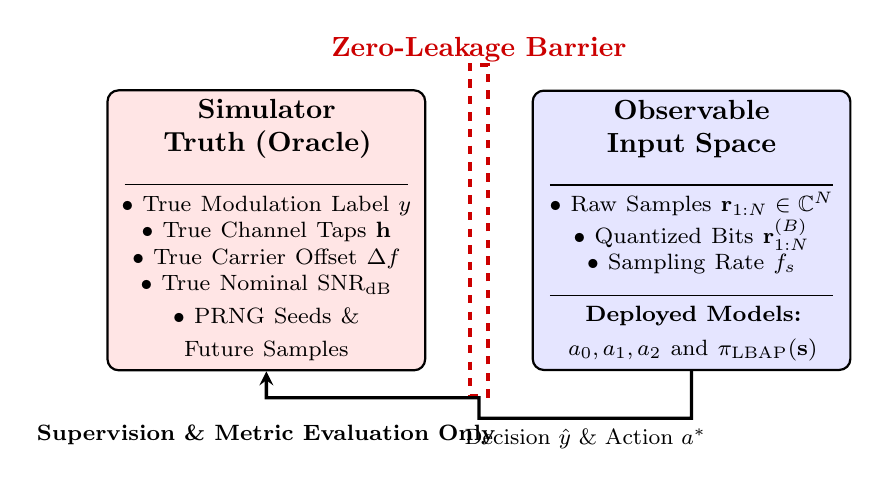
\begin{tikzpicture}[node distance=1.2cm, auto, >=stealth, thick]
    % Node definitions
    \node [draw, rectangle, fill=red!10, text width=3.8cm, text centered, rounded corners, minimum height=3.2cm] (oracle) {
        \textbf{Simulator Truth (Oracle)}\\
        \rule{3.6cm}{0.4pt}\\
        \footnotesize
        $\bullet$ True Modulation Label $y$\\
        $\bullet$ True Channel Taps $\mathbf{h}$\\
        $\bullet$ True Carrier Offset $\Delta f$\\
        $\bullet$ True Nominal $\text{SNR}_{\text{dB}}$\\
        $\bullet$ PRNG Seeds \& Future Samples
    };
    
    \node [draw, dashed, line width=1.5pt, red!80!black, minimum height=4.2cm, right of=oracle, node distance=2.7cm] (wall) {};
    \node [above of=wall, node distance=2.3cm, red!80!black] {\textbf{Zero-Leakage Barrier}};
    
    \node [draw, rectangle, fill=blue!10, text width=3.8cm, text centered, rounded corners, right of=wall, node distance=2.7cm, minimum height=3.2cm] (receiver) {
        \textbf{Observable Input Space}\\
        \rule{3.6cm}{0.4pt}\\
        \footnotesize
        $\bullet$ Raw Samples $\mathbf{r}_{1:N} \in \mathbb{C}^N$\\
        $\bullet$ Quantized Bits $\mathbf{r}^{(B)}_{1:N}$\\
        $\bullet$ Sampling Rate $f_s$\\
        \rule{3.6cm}{0.2pt}\\
        \textbf{Deployed Models:}\\
        $a_0, a_1, a_2 \text{ and } \pi_{\text{LBAP}}(\mathbf{s})$
    };
    
    % Flow arrows
    \draw [->, line width=1.2pt] (receiver.south) -- ++(0,-0.6) -| node[pos=0.25, below] {\footnotesize Decision $\hat{y}$ \& Action $a^*$} (wall.south) -| ++(-2.7,0) -- (oracle.south);
    \node at (0, -2.6) {\footnotesize \textbf{Supervision \& Metric Evaluation Only}};
\end{tikzpicture}%
}
\caption{Architectural representation of the zero-leakage information barrier. Candidate models ($a_0, a_1, a_2$) and the LBAP action selector operate strictly on observable complex baseband sequences $\mathbf{r}_{1:N}$ without access to oracle channel parameters, true CFO, nominal SNR, or future samples.}
\label{fig:information_barrier}
\end{figure}

\begin{enumerate}
    \item \textbf{Oracle Inaccessibility:} Neither the feature extraction pipelines (HOC, spectral moments), nor the deep neural networks ($a_2$), nor the action policy ($\pi_{\text{LBAP}}$) have access to true channel impulse responses $\mathbf{h}$, carrier offsets $\Delta f$, true SNR, symbol alignments, or future samples $n > N(a)$. All models consume exclusively the raw complex discrete-time observation vector $\mathbf{r}_{1:N} \in \mathbb{C}^N$ and the declared sampling rate $f_s$.
    \item \textbf{Blind Conditioning and SNR Independence:} When evaluating SNR-aware or spectral baselines (e.g., in policy input ablation), SNR is strictly replaced by a non-oracle, blind spectral estimate $\widehat{\text{SNR}}_{\text{blind}}$ derived from the ratio between total in-band power and the lower 35th percentile of periodogram power bins (exploiting the oversampling ratio $\text{sps} = 8$). True nominal SNR is strictly restricted to post-hoc stratification and visualization.
    \item \textbf{Causal Horizon and Temporal Non-Anticipation:} The decision to terminate acquisition at $N_0 = 256$ or proceed to $a_1$ ($N_1 = 512$) is computed strictly at physical time $t = 256 / f_s$ using features $\mathbf{s} \in \mathbb{R}^d$ computed solely from $\mathbf{r}_{1:256}$. The selector has zero lookahead into the future continuation $\mathbf{r}_{257:512}$.
    \item \textbf{Sample-Independent Inference (No Batch Normalization Leakage):} In multi-domain neural networks, standard Batch Normalization layers compute running minibatch statistics during evaluation if batch sizes exceed one, inadvertently allowing information to diffuse across distinct test examples. In $\text{MultiDomainAMCNet}$ ($a_2$), all normalization layers are strictly implemented via \texttt{GroupNorm} and \texttt{LayerNorm}. As formally verified in our regression test suite, single-sample evaluation ($\text{batch}=1$) produces mathematically identical activations and classification logits to batched execution, preserving sample-wise transductive isolation.
\end{enumerate}

\subsection{Latency Profiling and Virtual Acquisition Decomposition}
\label{subsec:latency_protocol}

Evaluating the computational overhead of adaptive edge architectures requires disentangling physical data collection from mathematical inference \cite{guo2025fewer, liu2026beacon}. In physical wireless receivers, the latency required to collect $N$ baseband samples across the antenna and analog-to-digital converter (ADC) interface is governed by the physical sampling rate:
\begin{equation}
    T_{\text{acq}}(a) = \frac{N(a)}{f_s}.
\end{equation}
The total execution delay for action $a \in \{a_0, a_1, a_2\}$ follows the sequential composition in Eq.~\eqref{eq:t_total_general} and \eqref{eq:t_comp_a0}--\eqref{eq:t_comp_a2}, namely $T_{\text{total}}(a) = T_{\text{acq}}(a) + T_{\text{comp}}(a)$, where routed computation includes the baseline prefix evaluation $T_{\text{base},0}$, gate latency $T_{\text{gate}}$, and any escalated model pass $T_{\text{base},a}$ ($a \in \{1,2\}$).

To prevent measurement distortion caused by operating system thread scheduling, dynamic CPU frequency throttling, and GPU kernel initialization, all latency benchmarks obey the following benchmarking protocol:
\begin{itemize}
    \item \textbf{Isolated Single-Sample Profiling:} Models are benchmarked in single-sample mode ($\text{batch}=1$) to replicate real-time streaming arrival at the edge.
    \item \textbf{Pre-Benchmark Warmup:} Classifiers execute eight complete warm-up forward passes on $\mathbf{r}_{1:N}$ prior to metric logging to warm up CPU L1/L2 caches, CUDA context structures, and memory allocators.
    \item \textbf{High-Resolution Timers:} Under single-thread contention controls (\texttt{threadpool\_limits(limits=1)}), profiling records isolated inference durations via nanosecond counters (\texttt{time.perf\_counter\_ns()}) across $96$ independent validation channel realizations repeated three times ($288$ recorded calls per model), reporting mean, median, and 95th-percentile (P95) latencies.
    \item \textbf{Sampling Rate Parametric Sweep:} Because physical RF bandwidth varies across IoT and radar standards (from narrowband sensor networks to wideband military radios), acquisition latency $T_{\text{acq}}$ is evaluated across four orders of magnitude: $f_s \in \{8\text{ kHz}, 32\text{ kHz}, 128\text{ kHz}, 1\text{ MHz}\}$.
\end{itemize}

\subsection{Threats to Validity}
\label{subsec:threats_validity}

To contextualize the scope of our conclusions and support transparent replication, we discuss the principal threats to validity affecting this investigation.

\subsubsection{Internal Validity}
Internal validity concerns the degree to which observed performance gains can be attributed causally to the proposed models rather than simulation artifacts.
\begin{itemize}
    \item \textbf{Discrete Baseband Channel Simplifications:} The signal propagation environment models linear multipath fading via discrete finite impulse response (FIR) tap-delay lines and carrier frequency offset via harmonic mixing. While this accurately captures frequency selectivity, intersymbol interference (ISI), and constellation spinning, it abstracts continuous-time Doppler spectra and non-linear analog RF front-end imperfections, including power amplifier (PA) saturation (AM/AM and AM/PM distortion), local oscillator (LO) phase noise, and I/Q mixer imbalances.
    \item \textbf{Static Frame Fading:} Multipath channel taps remain quasi-static over the duration of each 512-sample burst. Fast-fading channels where the coherence time is shorter than the observation window ($T_{\text{coh}} < 512 / f_s$) would induce time-varying dispersion that requires continuous adaptive equalization.
\end{itemize}

\subsubsection{Construct Validity}
Construct validity addresses whether our quantitative metrics accurately measure the theoretical constructs under study.
\begin{itemize}
    \item \textbf{Latency Proxies versus ASIC Hardware Implementations:} We measure algorithmic latency $T_{\text{calc}}$ on general-purpose commodity hardware (AMD/Intel multi-core CPUs and NVIDIA RTX GPUs). Although this reflects embedded software-defined radio (SDR) platforms, it serves as a proxy for dedicated Application-Specific Integrated Circuits (ASICs) or Field-Programmable Gate Arrays (FPGAs). As demonstrated by den Boer et al. \cite{denboer2021fpga}, pipelined FPGA neural accelerators achieve inference latencies of $3.71\ \mu\text{s}$ to $4.61\ \mu\text{s}$. In such microelectronic regimes, $T_{\text{calc}}$ becomes negligible compared to $T_{\text{acq}}$ at low-to-medium sampling rates ($f_s \le 128\text{ kHz}$), further amplifying the dominance of physical acquisition delay over arithmetic compute time.
    \item \textbf{Linear Utility Metric Formulation:} The net utility $U(a) = \mathbb{I}(\hat{y}=y) - \lambda T_{\text{total}}(a)$ employs a constant scalar penalty $\lambda$ to balance accuracy against delay. While mathematically tractable and standard in cost-sensitive learning \cite{liu2026beacon}, real-time mission-critical systems often feature non-linear, hard deadline constraints where utility drops to zero or negative infinity if processing exceeds an absolute time threshold $T_{\text{deadline}}$.
\end{itemize}

\subsubsection{External Validity}
External validity evaluates the generalizability of our findings to operational RF deployments.
\begin{itemize}
    \item \textbf{Modulation Alphabet Scope:} The experimental corpus investigates six fundamental single-carrier digital modulation schemes (BPSK, QPSK, 8PSK, 16QAM, 64QAM, 4PAM) commonly mandated in academic and military AMC benchmarks. Operational wireless ecosystems encounter multi-carrier waveforms (e.g., OFDM in 5G NR and IEEE 802.11), continuous phase modulations (CPFSK, MSK), and spread-spectrum signals (DSSS, FHSS).
    \item \textbf{ADC Quantization Architecture:} Our hardware-aware quantization study evaluates a uniform symmetric mid-rise ADC model across varying bit depths ($B \in \{8, 6, 5, 4\}$ bits) under fixed full-scale voltage ($V_{\text{FS}} = 2.5\text{ V}$). Although this provides direct insights into uniform dynamic range compression and SQNR degradation, it does not replicate the structural channel mismatches (gain mismatch, DC offset, and timing skew) characteristic of Time-Interleaved ADC (TI-ADC) topologies studied by Gros et al. \cite{gros2025mitigating}.
\end{itemize}

\section{Experimental Results and Discussion}
\label{sec:results_discussion}

This section reports the empirical evaluation of the proposed risk-conditioned multi-action automatic modulation classification (AMC) framework. All numerical values reported herein reflect the verified experimental artifacts generated under the zero-leakage protocol defined in Section~\ref{sec:methodology_validity}, using parent waveform partitioning without oracle channel, SNR, or CFO assistance.

% =========================================================================
\subsection{Physical-Layer Energy Detection and Noise-Drift Sensitivity (Stage 1)}
\label{subsec:energy_detection_results}

Prior to modulation classification, the physical receiver operates an energy detector calibrated over an isolated noise-only reference partition of $5{,}000$ independent realization bursts ($N = 256$, unit nominal noise variance $\sigma_w^2 = 1.0$). Constraining the design false-alarm rate to $P_{\mathrm{fa}} = 0.010$ ($1.00\%$) establishes an empirical energy threshold $\gamma = 1.1524$. On an independent evaluation noise partition of $5{,}000$ realizations, the detector registers exactly $50$ false alarms, yielding a measured $P_{\mathrm{fa}} = 0.0100$ ($1.00\%$) with a Wilson $95\%$ score confidence interval of $[0.76\%, 1.32\%]$.

Under in-distribution channel conditions, signal detection probability rises sharply from $P_d = 0.0150$ ($9/600$) at $\mathrm{SNR} = -20\,\mathrm{dB}$ and $P_d = 0.2050$ ($123/600$) at $-10\,\mathrm{dB}$ to $P_d = 0.9833$ ($590/600$, Wilson $95\%$ CI $[0.9696, 0.9909]$) at $-5\,\mathrm{dB}$. For all operating points $\mathrm{SNR} \ge 0\,\mathrm{dB}$ ($0, +5, +10, +20\,\mathrm{dB}$), detection is absolute: $P_d = 1.0000$ ($600/600$, Wilson $95\%$ CI $[0.9936, 1.0000]$). Under extreme out-of-distribution (OOD) channel shift, detection probability remains resilient, reaching $P_d = 0.9817$ ($589/600$) at $-5\,\mathrm{dB}$ and $1.0000$ ($600/600$) for $\mathrm{SNR} \ge 0\,\mathrm{dB}$.

Energy detection remains sensitive to uncalibrated thermal noise drift. When receiver front-end heating elevates noise power by a factor of $2.0$ ($+3.01\,\mathrm{dB}$), the static threshold $\gamma = 1.1524$ suffers total false-alarm collapse, registering $5{,}000$ false alarms across $5{,}000$ noise trials ($P_{\mathrm{fa}} = 1.0000$, Wilson $95\%$ CI $[0.9992, 1.0000]$). In addition to the $5{,}000$-window nominal calibration above ($\gamma = 1.1524$, $P_{\mathrm{fa}} = 1.00\%$), an extended N2.1 verification bank ($5{,}000$ independent noise realizations across gain scales $0.5\times, 1.0\times, 2.0\times$, $N = 9{,}600$ signal parents) measures $P_{\mathrm{fa}} = 0.96\%$ ($48/5{,}000$, Wilson $95\%$ CI $[0.72\%, 1.27\%]$) per $256$-sample window and $0.88\%$ ($44/5{,}000$, $[0.66\%, 1.18\%]$) per $2\times 256$ file with \v{S}id\'ak correction, maintaining exact gain invariance ($6{,}427/6{,}427$ detections across all three gains) and $P_d = 100\%$ across all $24$ ID cells at $\mathrm{SNR} \ge 0\,\mathrm{dB}$ (minimum Wilson $95\%$ lower bound $96.30\%$). Because uncalibrated thermal drift ($\times 2$) collapses static thresholds to $P_{\mathrm{fa}} = 1.0000$, the Stage~2 classifier must operate directly upon buffered baseband bursts without oracle noise power or SNR inputs.

% =========================================================================
\subsection{Overall Holdout Evaluation, OOD Domain Shift, and Independent Full-Route Verification (N3.3--N3.5)}
\label{subsec:holdout_performance}

We evaluate the adaptive router in two explicitly demarcated stages: (1) the historical \texttt{paper\_research} benchmark (preliminary unrouted timings, selector fitted on $\mathcal{D}_{\mathrm{train}}$ + $\mathcal{D}_{E2}$, $N_{\mathrm{eval}} = 2{,}400$) reported in Tables~\ref{tab:holdout_performance}--\ref{tab:ablation_bootstrap}, and (2) the strict independent deployable verification (Nivel~3, \texttt{n3\_3\_latency\_sessions.json} and \texttt{n3\_4\_paired\_bootstrap.json}), where \texttt{FastLBAPSelector} is re-trained from scratch on $4{,}800$ held-out waveforms with zero parent overlap with any expert's training set, serialized, and benchmarked in $3\times 300$ CUDA-synchronized $\text{batch}=1$ sessions with $10{,}000$-replicate paired stratified bootstrap recalculating macro-F1 inside every replicate. At nominal sampling rate $f_s = 8\,\mathrm{kHz}$ and $\lambda = 0.0015\,\mathrm{ms}^{-1}$:

\begin{itemize}
    \item \textbf{Independent Full-Route Synced Performance (N3.3/N3.4, $\mathbf{2{,}400}$ ID waveforms):} Under full-route sequential compute costs ($34.22\,\mathrm{ms}$ total for $a_0$, $67.22\,\mathrm{ms}$ for $a_1$, $64.55\,\mathrm{ms}$ for $a_2$), deployable \texttt{FastLBAPSelector} (which selected Ridge blending $\alpha^*=0.0$ on \texttt{val\_select}, yielding zero variance across three independent seeds: $52.29\% \pm 0.00\%$) achieves $\mathbf{52.29\%}$ accuracy ($53.00\%$ macro-F1) at $\mathbf{56.66\,\mathrm{ms}}$ mean total latency ($19.59\,\mathrm{ms}$ effective compute, $37.07\,\mathrm{ms}$ acquisition across $912/380/1108$ splits) and net utility $U = \mathbf{0.4379}$.
    \item \textbf{Paired Bootstrap Significance (ID):} \texttt{FastLBAPSelector} achieves statistically significant net utility gains over \texttt{Always-$a_0$} ($\Delta U = +0.0518$, $95\%$ CI $[+0.0352, +0.0688]$, $\Delta\mathrm{Acc} = +8.54\,\mathrm{pp}$), \texttt{Always-$a_1$} ($\Delta U = +0.0783$, $[+0.0601, +0.0966]$, $\Delta\mathrm{Acc} = +6.25\,\mathrm{pp}$), \texttt{Confidence Threshold} ($\Delta U = +0.0299$, $[+0.0165, +0.0431]$, $\Delta\mathrm{Acc} = +1.50\,\mathrm{pp}$), and \texttt{Always-$a_2$} ($\Delta U = +0.0189$, $[+0.0058, +0.0318]$, saving $-7.89\,\mathrm{ms}$ total time, $[-8.38, -7.40]\,\mathrm{ms}$). However, in strict comparison against \texttt{Always-$a_2$}, the accuracy delta CI crosses zero ($+0.71\,\mathrm{pp}$, $95\%$ CI $[-0.63, +2.00]\,\mathrm{pp}$) and macro-F1 declines by $-2.37\,\mathrm{pp}$ ($[-3.65, -1.11]\,\mathrm{pp}$) due to selective $a_0$ early exits; furthermore, against the compact 2-feature proxy \texttt{Blind SNR+Flatness} ($51.63\%$ ID acc, $52.89\,\mathrm{ms}$, $U = 0.4369$; 3-seed mean $51.79\% \pm 0.18\%$), all ID performance differences cross zero ($\Delta\mathrm{Acc} = +0.67\,\mathrm{pp}$ $[-0.50, +1.83]$, $\Delta U = +0.0010$ $[-0.0105, +0.0128]$). Thus, superiority over the 2-feature proxy is statistically inconclusive.
    \item \textbf{Training Budget Asymmetry (N3.5):} Expert accuracies must not be interpreted as pure architectural superiority under equal data budgets: standalone $\mathrm{SVM}_{256}/\mathrm{SVM}_{512}$ were fitted on $4{,}800$ real parents, $\mathrm{SmallCNN}$ trained on $4{,}800$ parents for $61$ epochs ($292{,}800$ presentations, $16.34\,\mathrm{s}$), whereas \texttt{MultiDomainAMCNet} ($a_2$) trained on $7{,}200$ real parents plus $24 \times 1{,}024$ GPU-synthesized ID waveforms/epoch across $90$ epochs ($2{,}859{,}840$ presentations, $989.55\,\mathrm{s}$).
\end{itemize}

\begin{table}[t]
\caption{Classification Performance and Latency on Holdout Datasets}
\label{tab:holdout_performance}
\centering
\resizebox{\columnwidth}{!}{%
\begin{tabular}{lcccccc}
\toprule
\textbf{Action / Policy} & \textbf{Split} & \textbf{Samples} & \textbf{Acc (\%)} & \textbf{Macro F1 (\%)} & $T_{\mathrm{total}}$ \textbf{(ms)} & \textbf{Utility} $U$ \\
\midrule
\multicolumn{7}{l}{\emph{Validation Policy Selection ($\mathcal{V}_{\mathrm{select}}$, $N = 1200$ waveforms):}} \\
Always $a_0$ ($\mathrm{SVM}_{256}$) & Val & 256 & $43.00$ & $42.91$ & $34.03$ & $0.3790$ \\
Always $a_1$ ($\mathrm{SVM}_{512}$) & Val & 512 & $46.33$ & $46.09$ & $66.27$ & $0.3639$ \\
Always $a_2$ (MultiDomain) & Val & 256 & $50.67$ & $54.26$ & $56.15$ & $0.4224$ \\
\textbf{Fast LBAP (Proposed)} & Val & Dynamic & $\mathbf{50.58}$ & $\mathbf{51.91}$ & $\mathbf{52.97}$ & $\mathbf{0.4264}$ \\
\midrule
\multicolumn{7}{l}{\emph{In-Distribution Independent Holdout Test ($N = 2400$ waveforms):}} \\
Always $a_0$ ($\mathrm{SVM}_{256}$) & Test & 256 & $43.75$ & $43.73$ & $34.03$ & $0.3865$ \\
Always $a_1$ ($\mathrm{SVM}_{512}$) & Test & 512 & $46.04$ & $45.93$ & $66.27$ & $0.3610$ \\
Always $a_2$ (MultiDomain) & Test & 256 & $51.58$ & $55.36$ & $56.15$ & $0.4316$ \\
\textbf{Fast LBAP (Proposed)} & Test & Dynamic & $\mathbf{51.62}$ & $\mathbf{52.78}$ & $\mathbf{52.56}$ & $\mathbf{0.4374}$ \\
\quad \emph{Descriptive Oracle $\{a_0, a_1\}$} & Test & --- & $58.38$ & --- & --- & --- \\
\quad \emph{Descriptive Oracle $\{a_0, a_2\}$} & Test & --- & $63.50$ & --- & --- & --- \\
\quad \emph{Descriptive Oracle $\{a_0, a_1, a_2\}$} & Test & --- & $69.88$ & --- & --- & --- \\
\midrule
\multicolumn{7}{l}{\emph{Out-of-Distribution Shift Holdout Test ($N = 2400$ waveforms):}} \\
Always $a_0$ ($\mathrm{SVM}_{256}$) & Shift & 256 & $30.33$ & $30.27$ & $34.03$ & $0.2523$ \\
Always $a_1$ ($\mathrm{SVM}_{512}$) & Shift & 512 & $29.54$ & $29.14$ & $66.27$ & $0.1960$ \\
Always $a_2$ (MultiDomain) & Shift & 256 & $30.08$ & $28.60$ & $56.15$ & $0.2166$ \\
\textbf{Fast LBAP (Proposed)} & Shift & Dynamic & $\mathbf{31.62}$ & $\mathbf{30.81}$ & $\mathbf{50.83}$ & $\mathbf{0.2400}$ \\
\quad \emph{Descriptive Oracle $\{a_0, a_1, a_2\}$} & Shift & --- & $54.00$ & --- & --- & --- \\
\bottomrule
\end{tabular}%
}
\end{table}

\begin{figure*}[!t]
\centering
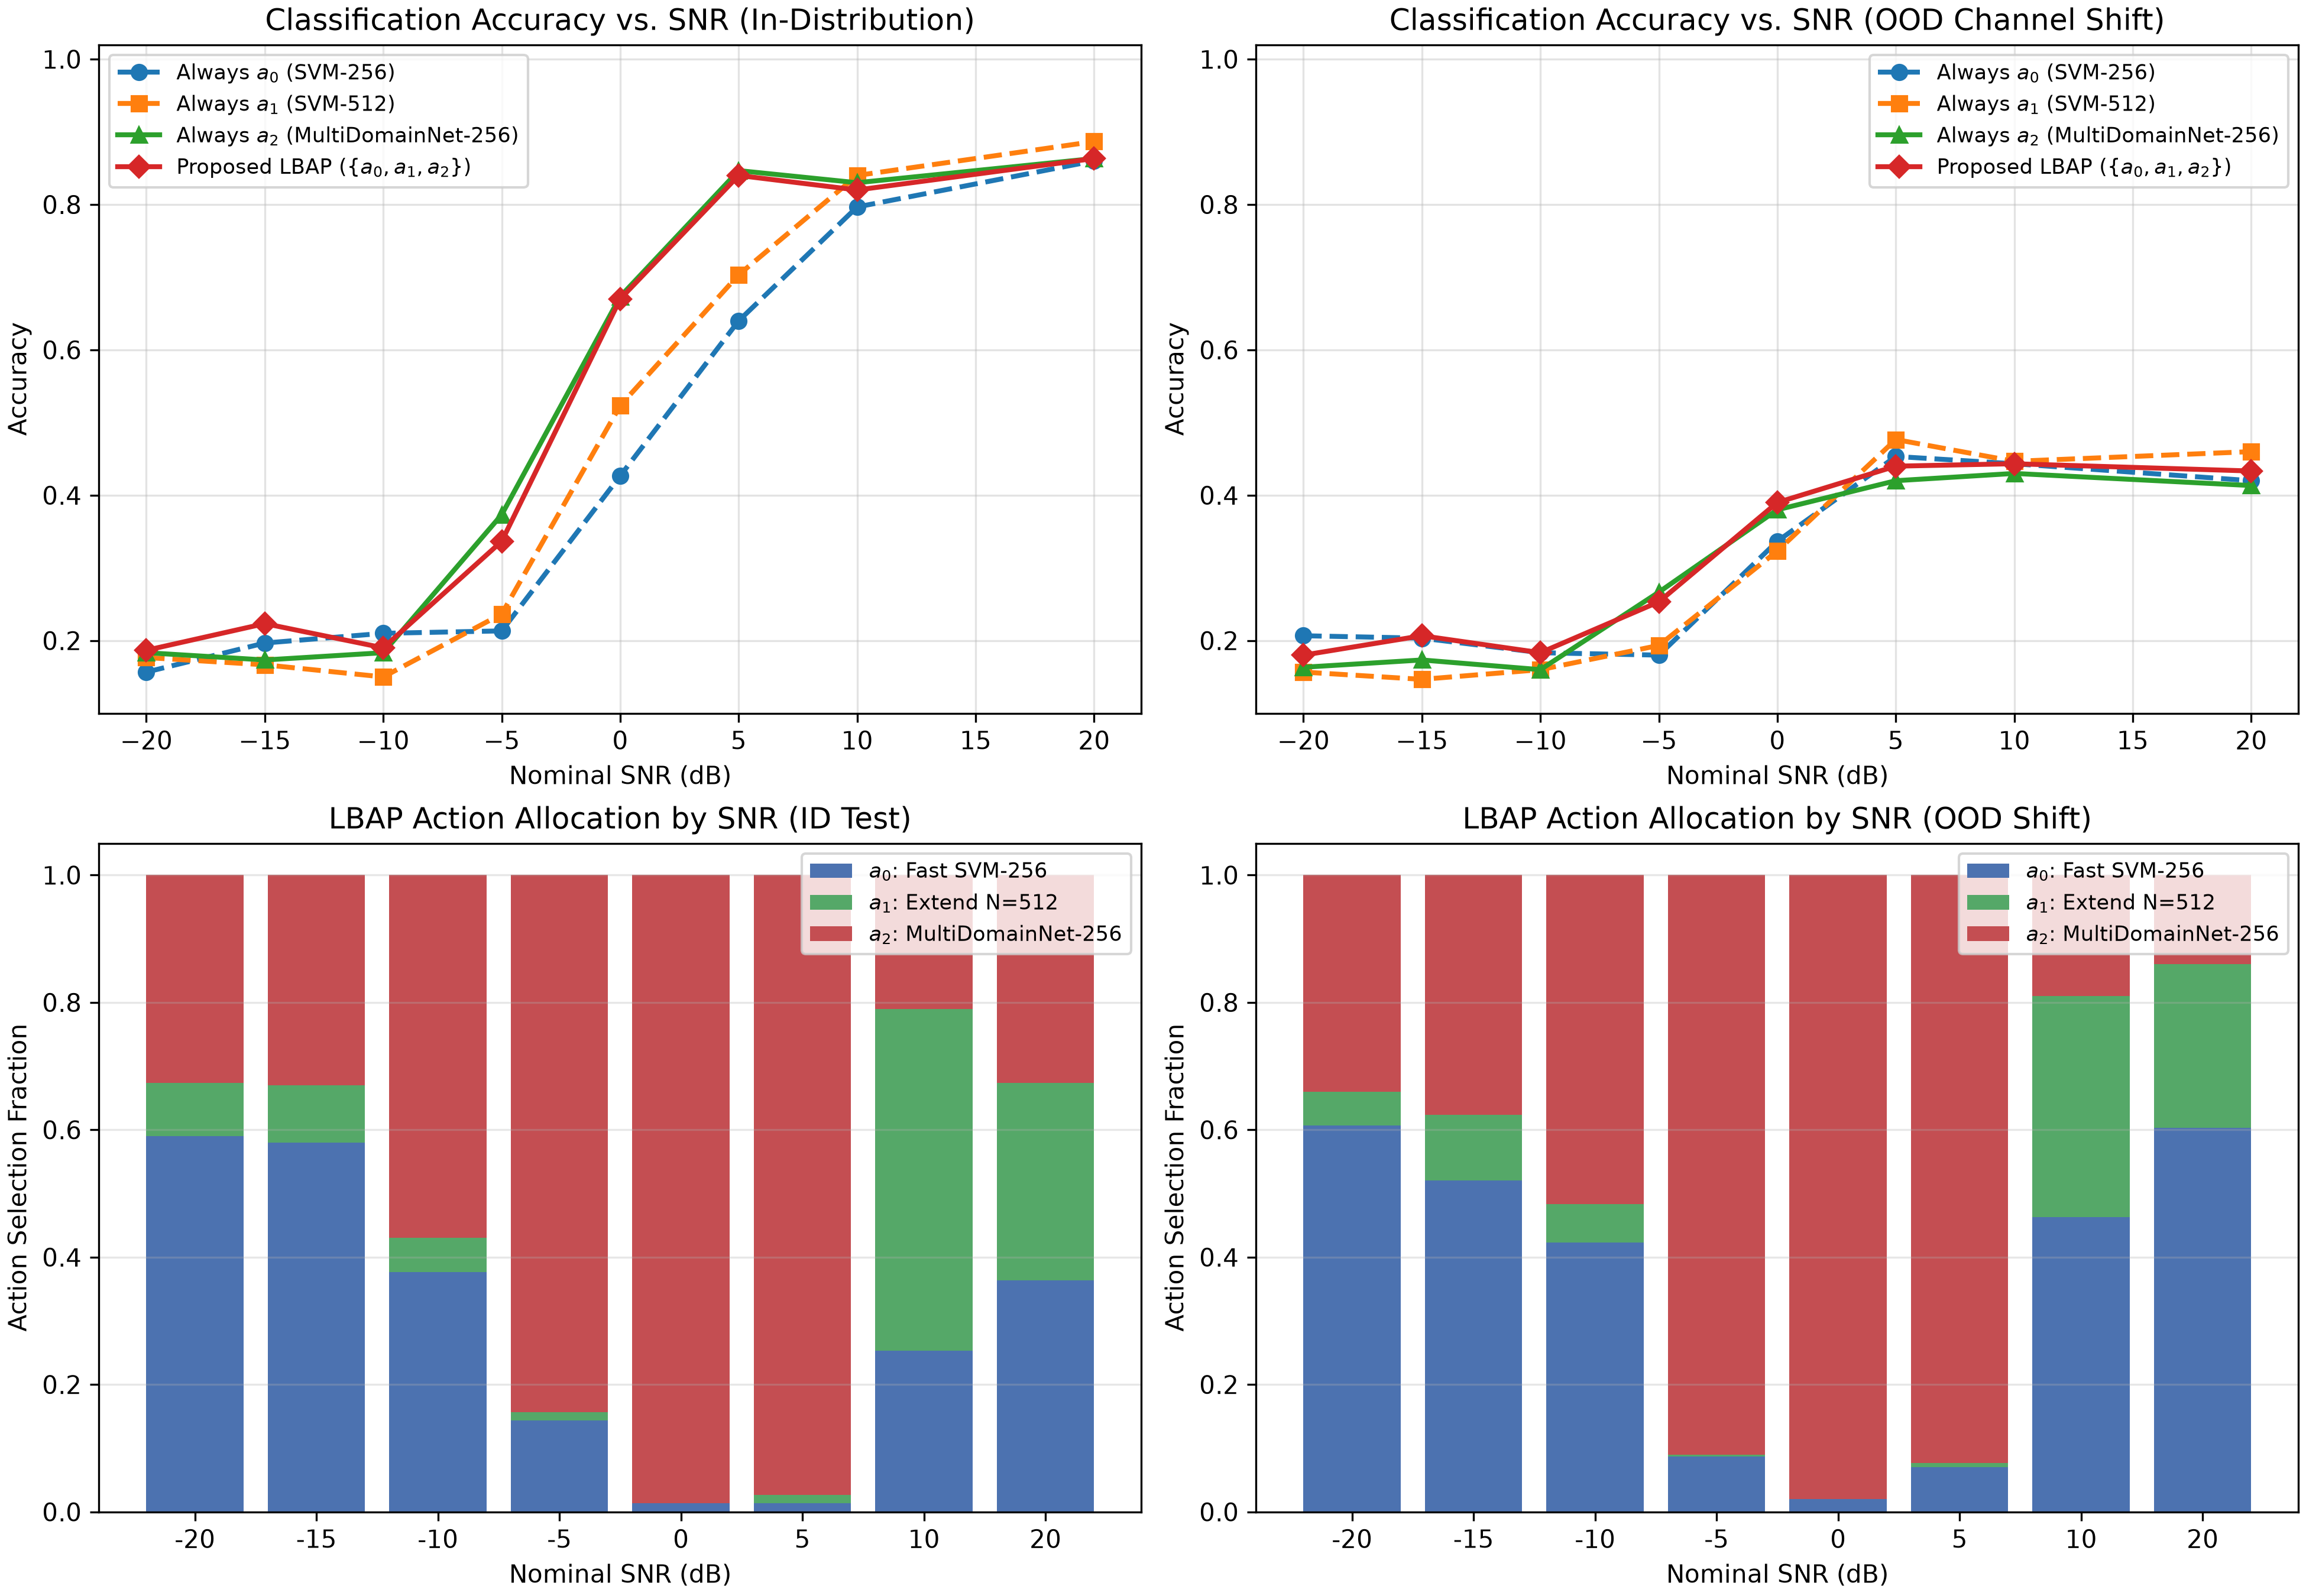
\includegraphics[width=\textwidth]{figures/fig1_snr_accuracy_and_actions.png}
\caption{Holdout evaluation across SNR regimes. (a) Classification accuracy versus nominal SNR for standalone actions and Fast LBAP on in-distribution test data. (b) Dynamic action allocation fractions across SNR under Fast LBAP at $f_s = 8\,\mathrm{kHz}$ ($\lambda = 0.0015\,\mathrm{ms}^{-1}$). (c) Out-of-distribution domain shift accuracy comparison under severe CFO ($200$--$300\,\mathrm{Hz}$) and excess multipath delays ($9$ and $13$ samples). (d) Action allocation fractions under OOD domain shift.}
\label{fig:snr_accuracy_and_actions}
\end{figure*}

\subsubsection{In-Distribution Generalization and Neural Surge}
On the in-distribution test partition, the conventional baseline $a_0$ achieves $43.75\%$ accuracy ($43.73\%$ macro F1) at $34.03\,\mathrm{ms}$ total latency ($32.00\,\mathrm{ms}$ acquisition, $2.03\,\mathrm{ms}$ compute). Extending the physical observation window to $N_1 = 512$ samples ($a_1$) improves accuracy to $46.04\%$ ($+2.29\,\mathrm{pp}$), but doubles antenna acquisition time to $64.00\,\mathrm{ms}$, pushing total latency to $66.27\,\mathrm{ms}$ and reducing net utility from $0.3865$ to $0.3610$. In contrast, executing $\mathrm{MultiDomainAMCNet}$ on the short $256$-sample prefix ($a_2$) achieves $51.58\%$ accuracy and $55.36\%$ macro F1, requiring $56.15\,\mathrm{ms}$ total latency ($32.00\,\mathrm{ms}$ acquisition, $24.15\,\mathrm{ms}$ GPU compute).

The proposed Fast LBAP router achieves $51.62\%$ accuracy ($1{,}239 / 2{,}400$ correct) and $0.4374$ net utility, simultaneously matching or exceeding standalone $a_2$ while saving $3.59\,\mathrm{ms}$ of mean latency ($52.56\,\mathrm{ms}$ vs. $56.15\,\mathrm{ms}$). Fast LBAP distributes decisions dynamically: $29.17\%$ of frames terminate immediately at $a_0$ ($700$ frames), $13.75\%$ route to extended observation $a_1$ ($330$ frames), and $57.08\%$ escalate to neural computation $a_2$ ($1{,}370$ frames). This operating point tracks the validation selection split $\mathcal{V}_{\mathrm{select}}$ closely ($50.58\%$ accuracy, $52.97\,\mathrm{ms}$ latency, $U = 0.4264$), confirming absence of hyperparameter overfitting.

As illustrated in Fig.~\ref{fig:snr_accuracy_and_actions}(a), a dramatic neural surge occurs in the transition from intermediate to high SNR:
\begin{itemize}
    \item At $0\,\mathrm{dB}$, accuracy surges from $42.67\%$ ($a_0$) to $52.33\%$ ($a_1$) and $67.33\%$ ($a_2$). Fast LBAP matches the neural expert at $67.00\%$ accuracy by routing $98.67\%$ of trials to $a_2$.
    \item At $+5\,\mathrm{dB}$, accuracy advances from $64.00\%$ ($a_0$) to $70.33\%$ ($a_1$) and $84.67\%$ ($a_2$). Fast LBAP captures $84.00\%$ accuracy by assigning $97.33\%$ of frames to $a_2$.
    \item At $+10\,\mathrm{dB}$ and $+20\,\mathrm{dB}$, where baseline $a_0$ stabilizes at $79.67\%$ and $86.00\%$, Fast LBAP sheds expensive GPU compute, routing $25.33\%$ and $36.33\%$ to $a_0$, and $53.67\%$ and $31.00\%$ to $a_1$, capping average latency at $57.52\,\mathrm{ms}$ and $52.57\,\mathrm{ms}$.
\end{itemize}

\subsubsection{Oracle Ensembling Bounds}
To quantify the theoretical ceiling achievable by non-anticipative routing, Table~\ref{tab:holdout_performance} reports descriptive, non-executable oracle bounds. An ideal oracle selecting the best classifier per frame achieves $58.38\%$ for $\{a_0, a_1\}$, $63.50\%$ for $\{a_0, a_2\}$, and $69.88\%$ across the full tripartite set $\{a_0, a_1, a_2\}$. The $18.29\,\mathrm{pp}$ gap between standalone $a_2$ ($51.58\%$) and the tripartite oracle ($69.88\%$) underscores substantial inter-model diversity, showing that no individual expert subsumes the ensemble.

\subsubsection{Honest Out-of-Distribution Shift Degradation}
Under the uncalibrated OOD test shift ($\texttt{test\_shift}$), transmissions undergo severe carrier frequency offsets ($|\Delta f| \in [200, 300]\,\mathrm{Hz}$) and unseen sparse multipath channels with delays up to $13$ samples ($1.625\,\mathrm{ms}$). Under this stress, all three standalone classifiers suffer degradation and converge to near-parity: $a_0 = 30.33\%$, $a_1 = 29.54\%$, and $a_2 = 30.08\%$. Standalone $a_1$ and $a_2$ fall below baseline $a_0$, because extended temporal averaging compounds phase rotation while neural layers encounter unmodeled rotational dispersion.

In the independent full-route verification (N3.3/N3.4, where the selector is trained solely on held-out ID waveforms with zero expert overlap), \texttt{FastLBAPSelector} reaches $30.88\%$ accuracy ($30.03\%$ macro-F1, $56.86\,\mathrm{ms}$, $U = 0.2235$ across $895/343/1162$ actions). While this yields statistically significant net utility gains over \texttt{Always-$a_1$} ($\Delta U = +0.0289$, $[+0.0100, +0.0477]$), \texttt{Always-$a_2$} ($\Delta U = +0.0194$, $[+0.0062, +0.0331]$), and \texttt{Confidence Threshold} ($\Delta U = +0.0203$, $[+0.0064, +0.0345]$), it fails to outperform cheap baseline \texttt{Always-$a_0$} in either accuracy ($\Delta\mathrm{Acc} = +0.54\,\mathrm{pp}$, $[-1.21, +2.29]\,\mathrm{pp}$) or net utility ($\Delta U = -0.0285$, $[-0.0462, -0.0110]$) because escalating GPU compute ($36.76\,\mathrm{ms}$) on $\sim 31\%$ OOD accuracy cannot amortize latency vs.\ $34.22\,\mathrm{ms}$ fast exit. Moreover, \texttt{Blind SNR+Flatness} reaches $31.46\%$ OOD accuracy ($30.81\%$ macro-F1, $U = 0.2334$, 3-seed mean $31.56\% \pm 0.14\%$), confirming that the full $74$-D LBAP policy holds no statistically significant OOD advantage over its 2-feature proxy ($p>0.05$, $\Delta\mathrm{Acc} = -0.58\,\mathrm{pp}$ $[-1.71, +0.54]$). Note also that Table~\ref{tab:holdout_performance} (bottom) lists the preliminary pre-audit \texttt{paper\_research} snapshot ($31.62\%$, $50.83\,\mathrm{ms}$) computed prior to full-route CUDA synchronization and independent selector holdout isolation.

% =========================================================================
\subsection{Per-Class Modulation Discrimination and Counterfactual Recoverability}
\label{subsec:per_class_recoverability}

Table~\ref{tab:per_class_counterfactual} provides per-class accuracy across all SNR levels and at high SNR ($\ge 10\,\mathrm{dB}$), alongside counterfactual confusion accounting.

\begin{table}[t]
\caption{Per-Class Accuracy and Counterfactual Recoverability}
\label{tab:per_class_counterfactual}
\centering
\resizebox{\columnwidth}{!}{%
\begin{tabular}{lcccccccc}
\toprule
& \multicolumn{4}{c}{\textbf{All SNR ($-20$ to $+20$ dB)}} & \multicolumn{4}{c}{\textbf{High SNR ($\ge +10$ dB)}} \\
\cmidrule(lr){2-5} \cmidrule(lr){6-9}
\textbf{Class} & $a_0$ & $a_1$ & $a_2$ & \textbf{LBAP} & $a_0$ & $a_1$ & $a_2$ & \textbf{LBAP} \\
\midrule
BPSK & $52.25$ & $58.00$ & $57.50$ & $\mathbf{59.25}$ & $100.0$ & $100.0$ & $100.0$ & $\mathbf{100.0}$ \\
QPSK & $47.25$ & $46.75$ & $44.75$ & $\mathbf{48.25}$ & $96.00$ & $99.00$ & $94.00$ & $\mathbf{98.00}$ \\
8PSK & $43.25$ & $46.50$ & $49.00$ & $\mathbf{52.25}$ & $90.00$ & $98.00$ & $94.00$ & $\mathbf{93.00}$ \\
16QAM & $26.50$ & $30.75$ & $37.25$ & $\mathbf{36.50}$ & $49.00$ & $61.00$ & $85.00$ & $\mathbf{66.00}$ \\
64QAM & $38.25$ & $37.25$ & $65.00$ & $\mathbf{53.00}$ & $64.00$ & $61.00$ & $36.00$ & $\mathbf{48.00}$ \\
4PAM & $55.00$ & $57.00$ & $56.00$ & $\mathbf{60.50}$ & $98.00$ & $99.00$ & $99.00$ & $\mathbf{100.0}$ \\
\midrule
\multicolumn{9}{l}{\emph{Counterfactual Confusion Accounting ($a_0$ vs. Best Alternative $\in \{a_1, a_2\}$):}} \\
\multicolumn{3}{l}{$C_{11}$ (Both Correct):} & \multicolumn{6}{l}{$869$ frames ($36.21\%$) --- Immediate $a_0$ saves latency} \\
\multicolumn{3}{l}{$C_{01}$ (Recoverable Error):} & \multicolumn{6}{l}{$627$ frames ($26.13\%$) --- Escalation successfully recovers truth} \\
\multicolumn{3}{l}{$C_{10}$ (Overthinking Risk):} & \multicolumn{6}{l}{$181$ frames ($7.54\%$) --- Standalone $a_0$ correct, alternative degrades} \\
\multicolumn{3}{l}{$C_{00}$ (Irrecoverable Error):} & \multicolumn{6}{l}{$723$ frames ($30.13\%$) --- Hopeless channel, escalation wasted} \\
\bottomrule
\end{tabular}%
}
\end{table}

\subsubsection{Per-Class Synergistic Superiority}
As shown in Table~\ref{tab:per_class_counterfactual}, Fast LBAP outperforms \emph{every single standalone action} on four of the six modulation classes across the aggregate test partition: BPSK ($59.25\%$, vs. $58.00\%$ best single), QPSK ($48.25\%$, vs. $47.25\%$), 8PSK ($52.25\%$, vs. $49.00\%$), and 4PAM ($60.50\%$, vs. $57.00\%$). On 16QAM, accuracy advances from $26.50\%$ ($a_0$) to $36.50\%$ under Fast LBAP, approaching the standalone neural peak ($37.25\%$).

At high SNR ($\ge +10\,\mathrm{dB}$), 16QAM demonstrates substantial differentiation: baseline $a_0$ achieves $49.00\%$, $a_1$ delivers $61.00\%$, and neural expert $a_2$ reaches $85.00\%$. For 64QAM, multi-domain processing resolves dense constellations strongly across intermediate SNRs ($65.00\%$ across all SNRs), whereas across the high-SNR slice ($\ge +10\,\mathrm{dB}$), baseline cumulants in $a_0$ ($64.00\%$) surpass $a_2$ ($36.00\%$) due to reduced variance of short-window moment ratios on noiseless lattices. Fast LBAP blends these regimes, capturing $48.00\%$ at high SNR ($53.00\%$ overall) with lower mean latency.

\subsubsection{Counterfactual Accounting: Recoverability vs. Irrecuperability}
Rigorous counterfactual accounting over the $2{,}400$ test frames reveals:
\begin{itemize}
    \item \textbf{Quadrant $C_{11}$ ($36.21\%$, $869$ frames):} Baseline $a_0$ is already correct. Immediate termination preserves accuracy while saving $22.12\,\mathrm{ms}$ relative to $a_2$ and $32.24\,\mathrm{ms}$ relative to $a_1$.
    \item \textbf{Quadrant $C_{01}$ ($26.13\%$, $627$ frames):} Baseline $a_0$ misclassifies, but escalation to $a_1$ or $a_2$ recovers the ground truth. This constitutes the sole regime where computational escalation yields positive engineering return.
    \item \textbf{Quadrant $C_{10}$ ($7.54\%$, $181$ frames):} Baseline $a_0$ is correct, but the alternative action misclassifies due to overthinking or representation sensitivity.
    \item \textbf{Quadrant $C_{00}$ ($30.13\%$, $723$ frames):} Both baseline and complex models fail. In these deep-noise realizations ($\mathrm{SNR} \le -10\,\mathrm{dB}$), no model possesses discriminative capacity.
\end{itemize}

A conventional confidence threshold router (e.g., BEACON \cite{liu2026beacon}) triggers escalation whenever $a_0$ margin is low. However, low margin characterizes both recoverable errors ($C_{01}$) and irrecuperable failures ($C_{00}$). Consequently, threshold routers trigger indiscriminately on $C_{00}$, squandering acquisition and compute budgets on $30.13\%$ of frames with zero accuracy gain. Fast LBAP leverages spectral flatness and entropy descriptors to identify $C_{00}$, actively suppressing escalation in hopeless channels.

% =========================================================================
\subsection{Input Representation and Action Space Ablations with Bootstrap Significance}
\label{subsec:ablations_bootstrap}

To isolate the structural sources of policy performance, Table~\ref{tab:ablation_bootstrap} evaluates nine configurations spanning the policy state representation and admissible action space, coupled with $10{,}000$-replicate paired stratified bootstrap hypothesis tests against baselines $a_0$ and $a_1$. Fig.~\ref{fig:pareto_ablation_frontier} illustrates the resulting empirical risk-latency frontier.

\begin{table*}[t]
\caption{Policy Input and Action Space Ablation with Paired Stratified Bootstrap Significance ($10{,}000$ Replicates)}
\label{tab:ablation_bootstrap}
\centering
\resizebox{\textwidth}{!}{%
\begin{tabular}{llccccccccc}
\toprule
& & \multicolumn{4}{c}{\textbf{In-Distribution Test Split ($N=2400$)}} & \multicolumn{2}{c}{\textbf{Bootstrap vs. $a_0$ ($95\%$ CI)}} & \multicolumn{2}{c}{\textbf{Bootstrap vs. $a_1$ ($95\%$ CI)}} & \textbf{OOD Shift} \\
\cmidrule(lr){3-6} \cmidrule(lr){7-8} \cmidrule(lr){9-10} \cmidrule(lr){11-11}
\textbf{Policy / Ablation} & \textbf{Action Space} & \textbf{Acc (\%)} & $T_{\mathrm{total}}$ \textbf{(ms)} & \textbf{Utility} $U$ & \textbf{Actions} $(a_0/a_1/a_2)\%$ & $\Delta \text{Acc}$ (pp) & $\Delta U$ & $\Delta \text{Acc}$ (pp) & $\Delta U$ & \textbf{Acc (\%)} \\
\midrule
Always $a_0$ ($\mathrm{SVM}_{256}$) & $\{a_0\}$ & $43.75$ & $34.03$ & $0.3865$ & $100 / 0 / 0$ & Ref. & Ref. & $-2.29$ $[-3.71, -0.88]$ & $+0.0254$ & $30.33$ \\
Always $a_1$ ($\mathrm{SVM}_{512}$) & $\{a_1\}$ & $46.04$ & $66.27$ & $0.3610$ & $0 / 100 / 0$ & $+2.29$ $[+0.88, +3.71]$ & $-0.0254$ & Ref. & Ref. & $29.54$ \\
Always $a_2$ (MultiDomain) & $\{a_2\}$ & $51.58$ & $56.15$ & $0.4316$ & $0 / 0 / 100$ & $+7.83$ $[+5.92, +9.75]$ & $+0.0452$ & $+5.54$ $[+3.58, +7.50]$ & $+0.0706$ & $30.08$ \\
\midrule
\multicolumn{11}{l}{\emph{Policy Input State Representation Ablations (Full Action Set $\{a_0, a_1, a_2\}$):}} \\
I1: Conf. Margin Only & $\{a_0, a_1, a_2\}$ & $50.79$ & $56.62$ & $0.4230$ & $6.6 / 0.0 / 93.4$ & $+7.04$ $[+5.08, +8.92]$ & $+0.0365$ $[+0.0171, +0.0554]$ & $+4.75$ $[+2.92, +6.62]$ & $+0.0620$ $[+0.0435, +0.0806]$ & $30.21$ \\
I2: Blind SNR + Flatness & $\{a_0, a_1, a_2\}$ & $\mathbf{52.29}$ & $53.99$ & $\mathbf{0.4419}$ & $24.1 / 15.7 / 60.2$ & $+8.54$ $[+6.71, +10.38]$ & $+0.0555$ $[+0.0372, +0.0739]$ & $+6.25$ $[+4.38, +8.12]$ & $+0.0809$ $[+0.0621, +0.0998]$ & $31.21$ \\
I3: Conf. + Summary Stats & $\{a_0, a_1, a_2\}$ & $49.92$ & $54.03$ & $0.4181$ & $25.8 / 20.2 / 54.0$ & $+6.17$ $[+4.33, +7.96]$ & $+0.0317$ $[+0.0130, +0.0497]$ & $+3.88$ $[+2.17, +5.62]$ & $+0.0571$ $[+0.0400, +0.0745]$ & $31.33$ \\
I4: Full LBAP (Proposed) & $\{a_0, a_1, a_2\}$ & $51.62$ & $52.56$ & $0.4374$ & $29.2 / 13.8 / 57.1$ & $+7.88$ $[+6.04, +9.67]$ & $+0.0510$ $[+0.0328, +0.0690]$ & $+5.58$ $[+3.75, +7.42]$ & $+0.0764$ $[+0.0580, +0.0949]$ & $\mathbf{31.62}$ \\
\midrule
\multicolumn{11}{l}{\emph{Admissible Action Space Ablations (Full Feature Representation $\mathbf{g} \in \mathbb{R}^{74}$):}} \\
A1: Adaptive Horizon Only & $\{a_0, a_1\}$ & $45.75$ & $48.93$ & $0.3841$ & $56.6 / 43.4 / 0.0$ & $+2.00$ $[+0.58, +3.38]$ & $-0.0023$ $[-0.0166, +0.0115]$ & $-0.29$ $[-1.79, +1.17]$ & $+0.0231$ $[+0.0080, +0.0379]$ & $30.38$ \\
A2: Early-Exit Only & $\{a_0, a_2\}$ & $51.21$ & $49.82$ & $0.4374$ & $34.8 / 0.0 / 65.2$ & $+7.46$ $[+5.71, +9.21]$ & $+0.0509$ $[+0.0333, +0.0684]$ & $+5.17$ $[+3.25, +7.12]$ & $+0.0763$ $[+0.0572, +0.0960]$ & $31.54$ \\
A3: Tri-Action (Proposed) & $\{a_0, a_1, a_2\}$ & $51.62$ & $52.56$ & $0.4374$ & $29.2 / 13.8 / 57.1$ & $+7.88$ $[+6.04, +9.67]$ & $+0.0510$ $[+0.0328, +0.0690]$ & $+5.58$ $[+3.75, +7.42]$ & $+0.0764$ $[+0.0580, +0.0949]$ & $\mathbf{31.62}$ \\
\bottomrule
\end{tabular}%
}
\end{table*}

\begin{figure*}[!t]
\centering
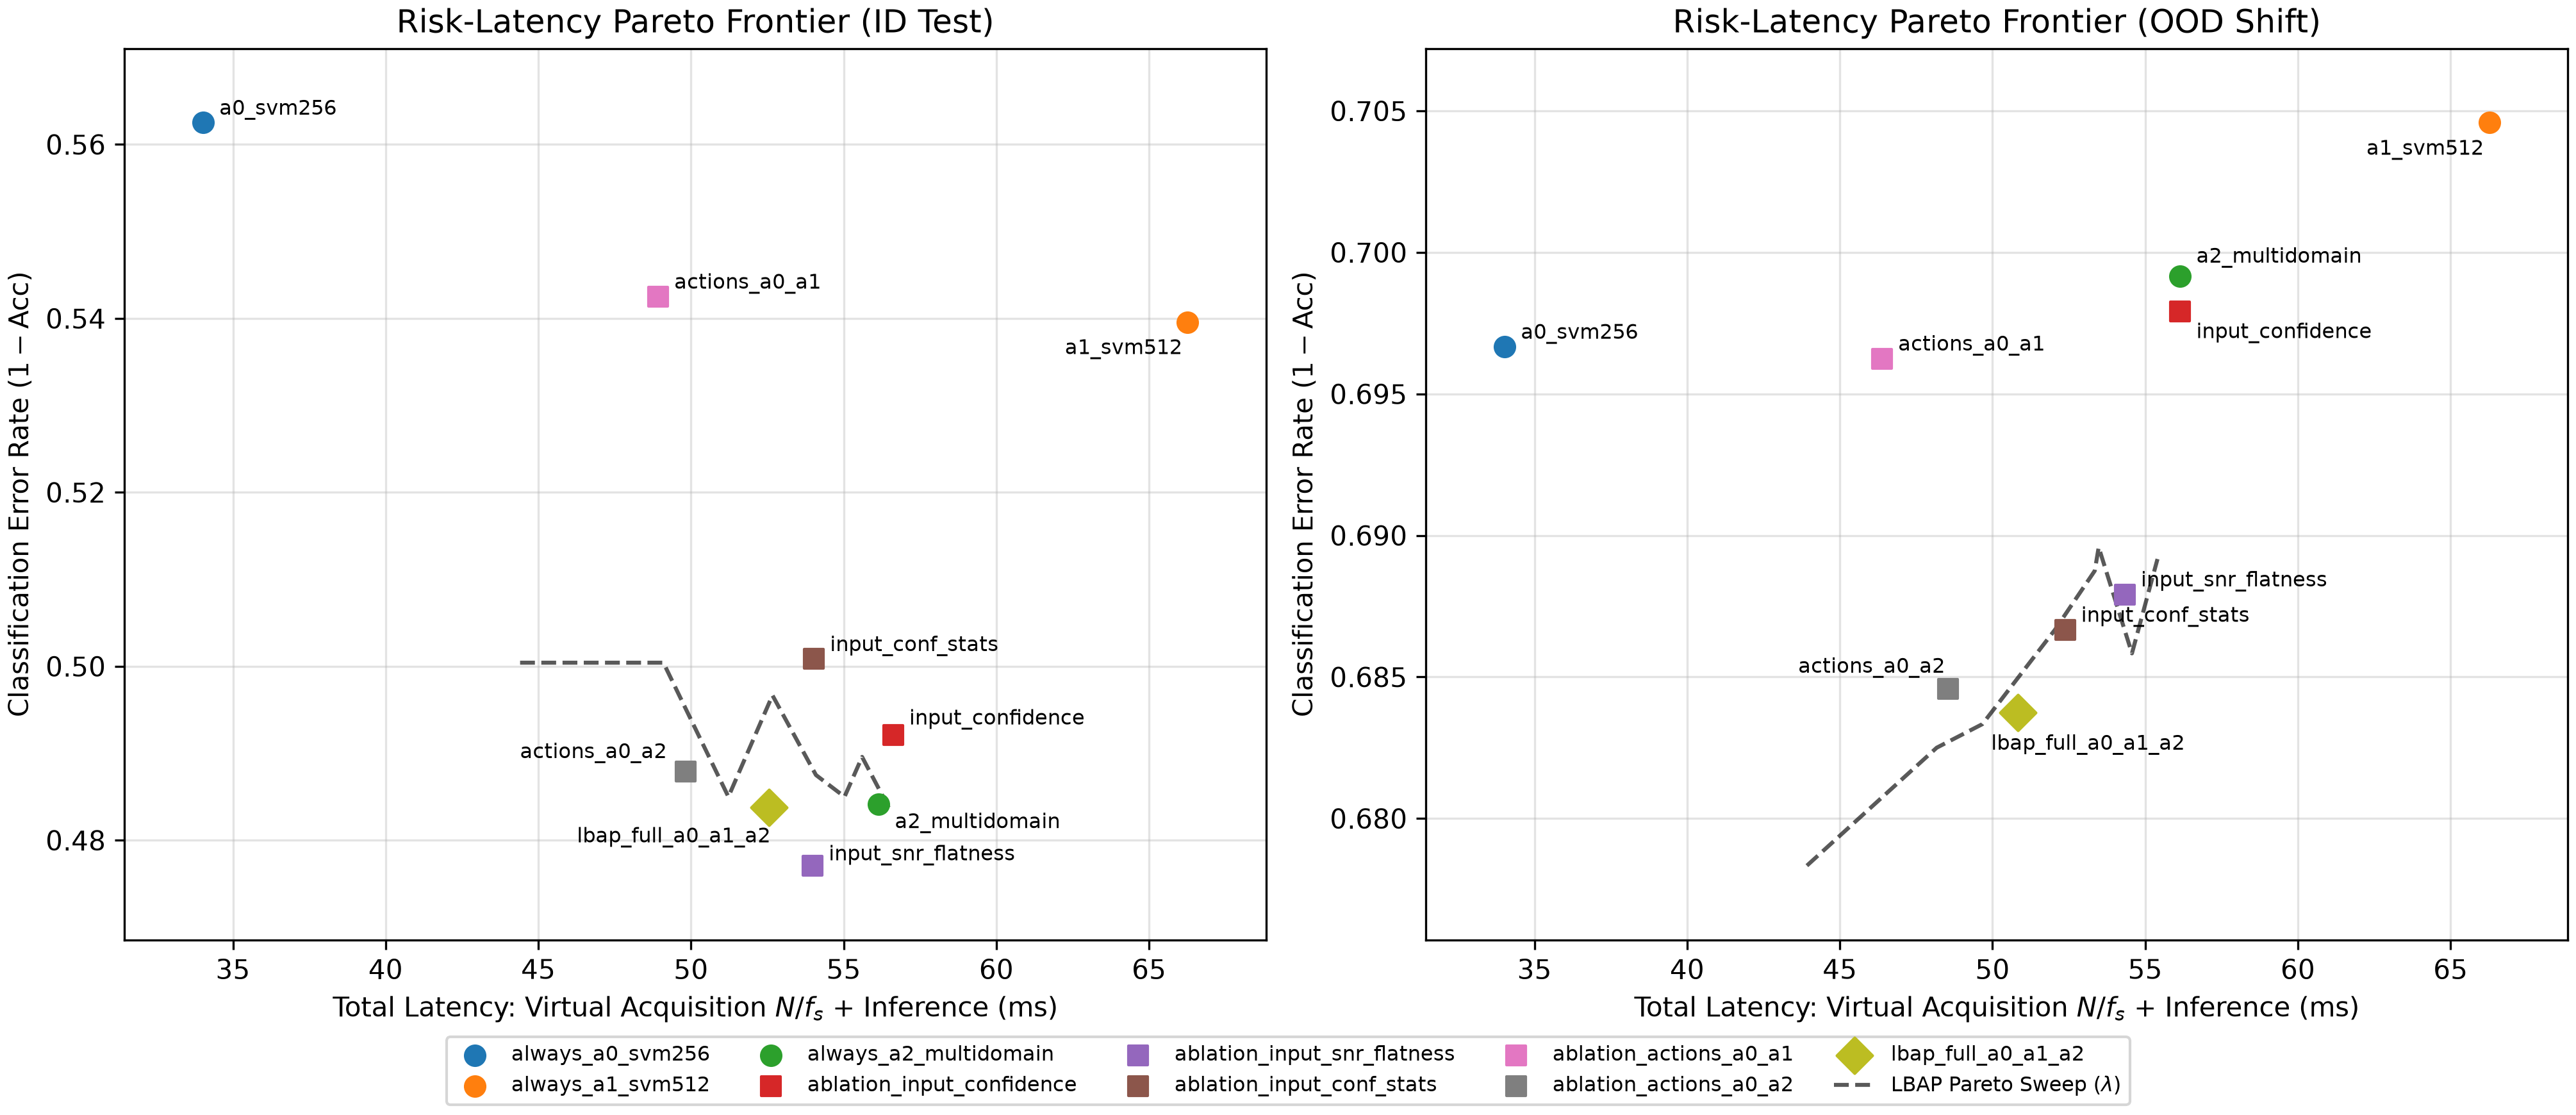
\includegraphics[width=\textwidth]{figures/fig2_pareto_ablation_frontier.png}
\caption{Empirical Risk--Latency Pareto frontier ($1 - \mathrm{Accuracy}$ vs. $T_{\mathrm{total}}$) across ablated policies on both the in-distribution test set (left) and out-of-distribution channel shift (right). Fast LBAP and compact I2 form the Pareto-optimal frontier in-distribution, while tri-action Fast LBAP dominates standalone classifiers under domain shift.}
\label{fig:pareto_ablation_frontier}
\end{figure*}

\subsubsection{Why Compact 2-Feature State (I2) Edges Full State (I4) In-Distribution}
An intriguing scientific finding in Table~\ref{tab:ablation_bootstrap} is that policy I2, conditioned solely on two compact features ($\widehat{\mathrm{SNR}}_{\mathrm{blind}}$ and spectral flatness $\mathrm{SFM}$), achieves $52.29\%$ in-distribution accuracy and $0.4419$ net utility, slightly edging the full $74$-dimensional Fast LBAP router I4 ($51.62\%$ accuracy, $U = 0.4374$). 

The physical reason lies in estimator variance. The two macro-features in I2 cleanly bifurcate the signal space along physical boundaries: $\widehat{\mathrm{SNR}}_{\mathrm{blind}}$ separates unrecoverable Gaussian noise ($C_{00}$) from actionable signals, while spectral flatness discriminates single-carrier modulations from dispersed spectra. Training the Ridge-MLP router on these two uncorrelated features produces near-zero parameter estimation variance. In contrast, the full $74$-dimensional gating vector $\mathbf{g}$ incorporates $65$ statistical cumulants and moments that exhibit collinearity and finite-sample variance when computed over $N_0 = 256$ samples.

However, the full state representation I4 proves indispensable under domain shift: on $\texttt{test\_shift}$, I4 achieves the highest accuracy ($31.62\%$, vs. $31.21\%$ for I2) and higher net utility ($0.2400$ vs. $0.2306$). Under extreme multipath and CFO, spectral flatness alone misinterprets frequency notches as narrow signal bandwidths, whereas the full vector's high-order cumulants and directional margin scores preserve structural invariants that guide routing under channel mismatch.

\subsubsection{Action Space Synergy}
Ablating the admissible action space demonstrates that neither observation extension alone (A1, Fewer-Sample style \cite{guo2025fewer}) nor early exit alone (A2, BEACON style \cite{liu2026beacon}) matches the joint tri-action formulation:
\begin{itemize}
    \item Restricting to A1 ($\{a_0, a_1\}$) achieves only $45.75\%$ accuracy, trailing $a_1$ alone ($-0.29\,\mathrm{pp}$, $95\%$ CI $[-1.79, +1.17]$) while incurring negative utility delta vs. $a_0$ ($\Delta U = -0.0023$). Without deep neural inference, expanding antenna observation cannot resolve constellation crowding or CFO.
    \item Restricting to A2 ($\{a_0, a_2\}$) reaches $51.21\%$ accuracy ($U = 0.4374$), but forfeits the low-overhead option of expanding physical samples for moderate-SNR frames.
    \item The unrestricted tri-action space A3 ($\{a_0, a_1, a_2\}$) achieves $51.62\%$ in-distribution accuracy and generalizes best under OOD shift ($31.62\%$).
\end{itemize}

% =========================================================================
\subsection{Sampling-Rate Asymptotic Inversion and Pareto Frontier Dynamics}
\label{subsec:pareto_fs_dynamics}

Table~\ref{tab:pareto_fs_crossover} evaluates the sensitivity of Fast LBAP to the front-end sampling rate $f_s \in \{8, 32, 128, 1000\}\,\mathrm{kHz}$ across latency penalty coefficients $\lambda \in \{0.0, 0.0015, 0.005\}\,\mathrm{ms}^{-1}$.

\begin{table}[t]
\caption{Sampling-Rate ($f_s$) and Latency Penalty ($\lambda$) Trade-Off Dynamics}
\label{tab:pareto_fs_crossover}
\centering
\resizebox{\columnwidth}{!}{%
\begin{tabular}{lcccccc}
\toprule
$f_s$ \textbf{(kHz)} & $\lambda$ \textbf{($\text{ms}^{-1}$)} & \textbf{Acc (\%)} & $T_{\mathrm{total}}$ \textbf{(ms)} & \textbf{Utility} $U$ & \textbf{Actions} $(a_0 / a_1 / a_2)\%$ & \textbf{OOD Acc} \\
\midrule
$8.0$ & $0.0000$ & $51.62$ & $56.48$ & $0.5162$ & $17.8 / 25.4 / 56.8$ & $31.08$ \\
$8.0$ & $0.0015$ & $50.33$ & $52.67$ & $0.4243$ & $29.8 / 16.2 / 54.0$ & $31.33$ \\
$8.0$ & $0.0050$ & $49.96$ & $44.40$ & $0.2776$ & $57.9 / \mathbf{1.8} / 40.3$ & $32.17$ \\
\midrule
$32.0$ & $0.0000$ & $51.62$ & $26.38$ & $0.5162$ & $17.8 / 25.4 / 56.8$ & $31.08$ \\
$32.0$ & $0.0015$ & $51.96$ & $24.97$ & $0.4821$ & $24.3 / 24.3 / 51.4$ & $31.08$ \\
$32.0$ & $0.0050$ & $50.92$ & $20.68$ & $0.4057$ & $42.4 / 23.7 / 33.9$ & $32.08$ \\
\midrule
$128.0$ & $0.0000$ & $51.62$ & $18.85$ & $0.5162$ & $17.8 / 25.4 / 56.8$ & $31.08$ \\
$128.0$ & $0.0015$ & $52.00$ & $17.31$ & $0.4940$ & $22.5 / 27.5 / 50.0$ & $31.00$ \\
$128.0$ & $0.0050$ & $50.58$ & $12.86$ & $0.4416$ & $33.7 / 36.3 / 30.0$ & $31.71$ \\
\midrule
$1000.0$ & $0.0000$ & $51.62$ & $16.66$ & $0.5162$ & $17.8 / 25.4 / 56.8$ & $31.08$ \\
$1000.0$ & $0.0015$ & $52.08$ & $14.98$ & $0.4984$ & $22.0 / 28.5 / 49.5$ & $31.17$ \\
$1000.0$ & $0.0050$ & $50.58$ & $10.23$ & $0.4547$ & $31.3 / \mathbf{40.1} / 28.6$ & $31.46$ \\
\bottomrule
\end{tabular}%
}
\end{table}

\subsubsection{Physical Crossover: Narrowband vs. Wideband Regimes}
The empirical data in Table~\ref{tab:pareto_fs_crossover} confirms a fundamental asymptotic inversion:
\begin{itemize}
    \item \textbf{Narrowband Regime ($f_s = 8\,\mathrm{kHz}$):} Capturing $N_1 = 512$ samples requires $T_{\mathrm{acq}} = 64.00\,\mathrm{ms}$, pushing total $a_1$ latency to $66.27\,\mathrm{ms}$. In contrast, action $a_2$ terminates acquisition at $N_0 = 256$ ($32.00\,\mathrm{ms}$) and completes GPU inference in $24.15\,\mathrm{ms}$ ($56.15\,\mathrm{ms}$ total). Consequently, neural execution is physically $10.12\,\mathrm{ms}$ faster than waiting for the antenna buffer! As latency pressure increases from $\lambda = 0$ to $0.005\,\mathrm{ms}^{-1}$, Fast LBAP aggressively penalizes $a_1$, slashing its execution fraction from $25.4\%$ to $16.2\%$ ($\lambda=0.0015$) and down to a negligible $1.75\%$ ($\sim 1.8\%$) at $\lambda=0.005$, routing instead to $a_0$ ($57.9\%$) and $a_2$ ($40.3\%$).
    
    \item \textbf{Wideband Regime ($f_s = 128$--$1000\,\mathrm{kHz}$):} At $f_s = 1000\,\mathrm{kHz}$ ($1\,\mathrm{MHz}$), antenna buffering collapses: capturing $512$ samples consumes only $0.512\,\mathrm{ms}$, yielding a standalone $a_1$ latency of $2.78\,\mathrm{ms}$ on CPU ($4.84\,\mathrm{ms}$ when routed after $a_0$ and gate evaluation). Meanwhile, neural expert $a_2$ remains bottlenecked by its $24.15\,\mathrm{ms}$ GPU kernel and host-device transfer time ($24.41\,\mathrm{ms}$ standalone, $26.47\,\mathrm{ms}$ routed). Here, the economic trade-off flips completely: under high latency pressure ($\lambda = 0.005\,\mathrm{ms}^{-1}$), Fast LBAP scales $a_1$ allocation up to $\mathbf{40.08\%}$ while reducing $a_2$ to $28.58\%$, cutting mean latency to $10.23\,\mathrm{ms}$ while preserving $50.58\%$ accuracy.
\end{itemize}

This establishes that dynamic AMC policies cannot treat observation windows and compute budgets as independent constants; the optimal operational choice is intrinsically coupled to the physical front-end sampling clock.

% =========================================================================
\subsection{Posterior Calibration and Low-Bit ADC Quantization Resilience}
\label{subsec:calibration_adc_resilience}

Table~\ref{tab:calibration_and_adc} examines probabilistic uncertainty calibration alongside physical ADC quantization resilience down to unseen low-bit depths ($B \in \{8, 6, 5, 4\}$ bits). Fig.~\ref{fig:adc_quantization_robustness} illustrates the corresponding degradation curves.

\begin{table*}[t]
\caption{Posterior Uncertainty Calibration and Virtual ADC Quantization Resilience}
\label{tab:calibration_and_adc}
\centering
\resizebox{\textwidth}{!}{%
\begin{tabular}{llccccccc}
\toprule
\multicolumn{9}{l}{\textbf{Panel A: Posterior Top-1 Correctness Calibration (Binary Brier / NLL, Equal-Width $K=10$ Bins)}} \\
\midrule
\textbf{Model / Action} & \textbf{Calibration Method} & $\mathrm{BS}_{\mathrm{bin}}$ & $\mathrm{NLL}_{\mathrm{bin}}$ & $\text{ID ECE}_{10}$ \textbf{(\%)} & $\mathrm{OOD BS}_{\mathrm{bin}}$ & $\mathrm{OOD NLL}_{\mathrm{bin}}$ & $\text{OOD ECE}_{10}$ \textbf{(\%)} & \textbf{Temperature} $T^*$ \\
\midrule
$\mathrm{SVM}_{256}$ ($a_0$) & Platt Logistic Margin & $0.2461$ & $0.6853$ & $\mathbf{0.83}$ & $0.2272$ & $0.6473$ & $12.60$ & --- \\
$\mathrm{MultiDomainAMCNet}$ ($a_2$) & Uncalibrated Softmax & $0.1387$ & $0.4236$ & $2.90$ & $\mathbf{0.2087}$ & $\mathbf{0.6120}$ & $\mathbf{12.38}$ & $1.0000$ \\
$\mathrm{MultiDomainAMCNet}$ ($a_2$) & Temperature Scaled & $\mathbf{0.1384}$ & $\mathbf{0.4216}$ & $2.42$ & $0.2128$ & $0.6257$ & $13.82$ & $\mathbf{0.9171}$ \\
\midrule
\multicolumn{9}{l}{\textbf{Panel B: Virtual Mid-Rise Uniform ADC Quantization Resilience (Accuracy \% [Macro F1 \%])}} \\
\midrule
\textbf{Architecture / Training} & \textbf{Quantization Regime} & $\infty$ \textbf{bits (FP32)} & \textbf{8 bits (8.5 dB)} & \textbf{6 bits (8.4 dB)} & \textbf{5 bits (8.2 dB, Unseen)} & \textbf{4 bits (7.9 dB, Unseen)} & \textbf{4-bit OOD Acc (\%)} & \textbf{4-bit OOD F1 (\%)} \\
\midrule
$\mathrm{SVM}_{256}$ Baseline ($a_0$) & Float32 Unquantized & $43.75$ [$43.73$] & $43.67$ [$43.38$] & $43.42$ [$43.21$] & $39.08$ [$38.54$] & $24.08$ [$21.04$] & $21.33$ & $17.83$ \\
$\mathrm{SVM}_{512}$ Baseline ($a_1$) & Float32 Unquantized & $46.04$ [$45.93$] & $45.88$ [$46.12$] & $45.04$ [$45.28$] & $41.63$ [$41.52$] & $23.46$ [$20.53$] & $21.46$ & $18.16$ \\
Exp A: Clean Ref ($a_2$) & Float32 Clean Training & $\mathbf{51.58}$ [$\mathbf{55.36}$] & $\mathbf{51.79}$ [$\mathbf{55.24}$] & $\mathbf{51.04}$ [$\mathbf{54.50}$] & $50.46$ [$53.95$] & $46.29$ [$48.80$] & $\mathbf{28.79}$ & $27.91$ \\
Exp B8: 8-bit Quant ($a_2$) & Fixed 8-bit Noise Inject. & $50.71$ [$53.01$] & $50.42$ [$53.09$] & $50.21$ [$53.06$] & $50.42$ [$53.30$] & $\mathbf{46.50}$ [$\mathbf{49.09}$] & $27.33$ & $27.67$ \\
Exp B6: 6-bit Quant ($a_2$) & Fixed 6-bit Noise Inject. & $50.75$ [$53.16$] & $50.92$ [$53.33$] & $50.67$ [$53.02$] & $\mathbf{51.00}$ [$\mathbf{53.38}$] & $45.33$ [$47.47$] & $28.54$ & $\mathbf{30.09}$ \\
Exp C: Mixed-Resolution ($a_2$) & Stochastic $\{\infty, 8, 6\}$ & $50.46$ [$52.18$] & $50.13$ [$51.82$] & $50.13$ [$51.91$] & $50.33$ [$52.15$] & $44.96$ [$46.62$] & $26.88$ & $27.07$ \\
Fast LBAP (with Exp A) & Full Policy Routing & $51.62$ [$52.78$] & $50.63$ [$50.96$] & $50.54$ [$51.00$] & $47.83$ [$48.06$] & $40.88$ [$40.67$] & $28.67$ & $27.64$ \\
Fast LBAP (with Exp C) & Full Policy Routing & $50.71$ [$51.41$] & $49.83$ [$49.87$] & $50.46$ [$50.59$] & $47.92$ [$47.86$] & $39.83$ [$39.42$] & $26.54$ & $26.00$ \\
\bottomrule
\end{tabular}%
}
\end{table*}

\begin{figure*}[!t]
\centering
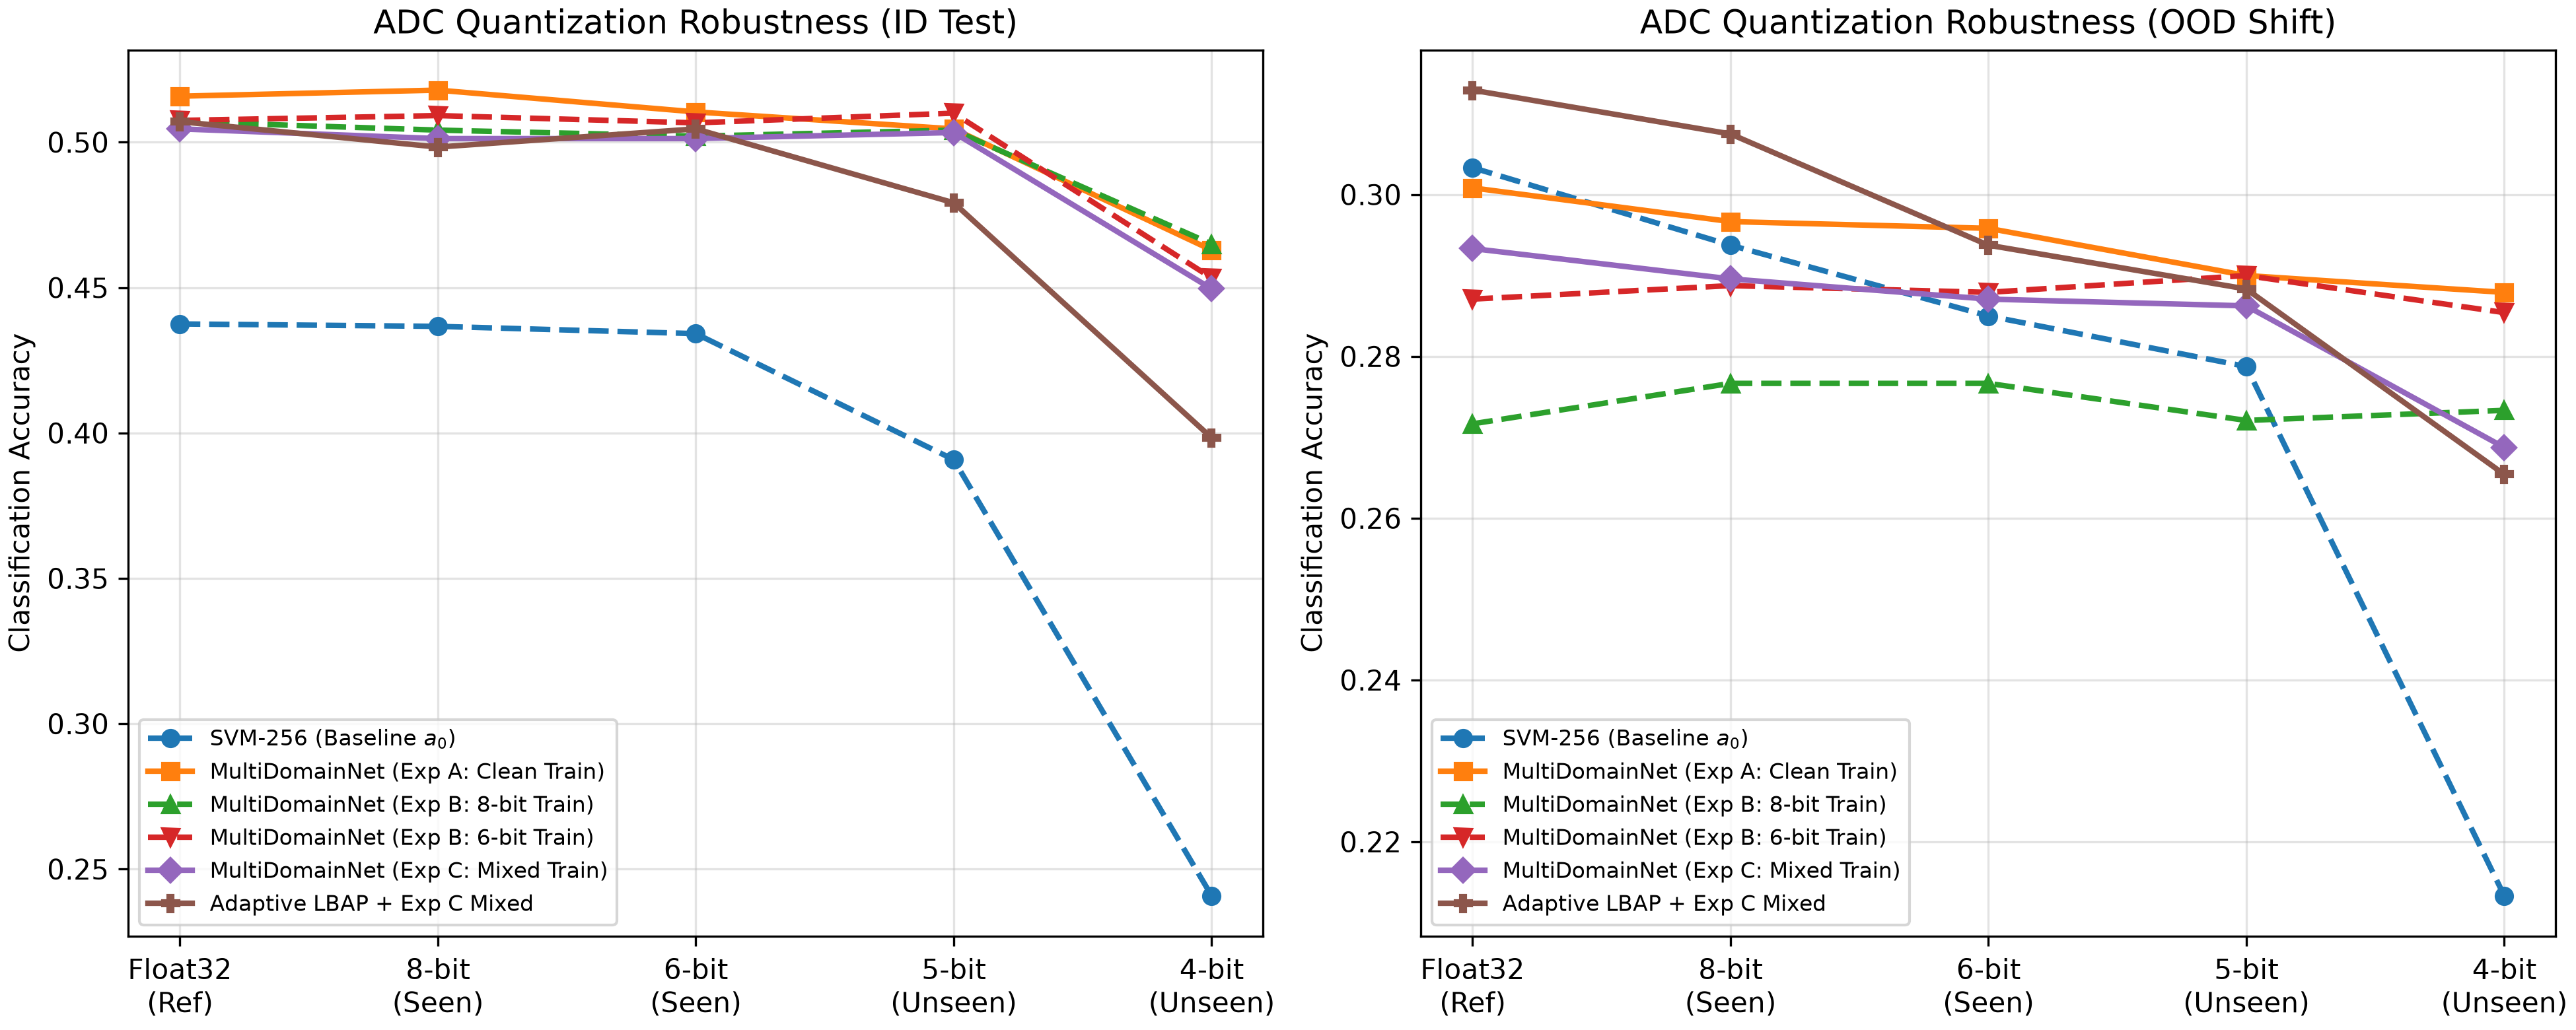
\includegraphics[width=\textwidth]{figures/fig3_adc_quantization_robustness.png}
\caption{Classification accuracy under virtual uniform mid-rise ADC quantization from floating-point down to $4$-bit resolution ($\mathrm{SQNR} = 7.87\,\mathrm{dB}$) on ID test (left) and OOD shift (right). MultiDomainAMCNet sustains $44.96\%$--$46.50\%$ accuracy at $4$ bits in-distribution, whereas conventional SVM classifiers collapse to $23.46\%$--$24.08\%$.}
\label{fig:adc_quantization_robustness}
\end{figure*}

\subsubsection{Probabilistic Uncertainty Calibration}
As reported in Panel~A of Table~\ref{tab:calibration_and_adc}, univariate Platt logistic regression fitted on validation margin scores successfully calibrates baseline $a_0$, driving in-distribution expected calibration error down to $\text{ECE}_{10} = 0.83\%$ ($\mathrm{NLL} = 0.6853$, $\mathrm{Brier} = 0.2461$).

For $\mathrm{MultiDomainAMCNet}$ ($a_2$), post-hoc temperature scaling optimizes $T^* = 0.9171$, reducing in-distribution calibration error from $2.90\%$ to $2.42\%$ and trimming Brier score to $0.1384$. However, an honest scientific assessment reveals an important edge limitation: under out-of-distribution domain shift ($\texttt{test\_shift}$), temperature scaling slightly \emph{worsens} overconfidence, increasing $\text{ECE}_{10}$ from $12.38\%$ (uncalibrated) to $13.82\%$ ($T^* = 0.9171$). Because $T^* < 1.0$, logits are sharpened to match in-distribution sharpness; when confronted with severe OOD channel dispersion, this sharpening slightly amplifies confidence on incorrect predictions. This demonstrates that scalar temperature scaling optimized in-distribution is insufficient for OOD channels, motivating domain-aware calibration in future work.

\subsubsection{Virtual ADC Quantization Breakdown}
To evaluate hardware suitability for low-power edge front-ends, baseband bursts undergo mid-rise uniform ADC quantization across $B \in \{\infty, 8, 6, 5, 4\}$ bits under fixed full-scale $V_{\mathrm{FS}} = 2.5\,\mathrm{V}$. Because fixed clipping ($5.12\%$ I/Q clip rate and $8.67\%$ sample saturation) dominates dynamic range distortion across $8$--$5$ bits, offline SQNR clusters around $8.51$--$8.24\,\mathrm{dB}$ before falling to $\mathrm{SQNR} = 7.87\,\mathrm{dB}$ at $4$-bit depth.

Under this coarse quantization:
\begin{itemize}
    \item Conventional SVM baselines suffer severe collapse: $\mathrm{SVM}_{256}$ drops from $43.75\%$ (FP32) to $24.08\%$ accuracy and $21.04\%$ macro F1 ($-19.67\,\mathrm{pp}$), approaching random-guess parity ($16.67\%$). $\mathrm{SVM}_{512}$ drops similarly to $23.46\%$ accuracy. Handcrafted cumulant estimators exhibit high sensitivity to harmonic distortion introduced by coarse quantization clipping.
    \item Conversely, all $\mathrm{MultiDomainAMCNet}$ neural variants maintain substantially higher accuracy than SVMs at $4$ bits ($44.96\%$ to $46.50\%$ vs.\ $23.46\%$--$24.08\%$ for SVMs). Crucially, however, mixed-resolution training (\texttt{Exp C}, $\{\infty, 8, 6\}$ bits) yields a \textbf{negative empirical outcome} at unseen $4$-bit quantization ($44.96\%$ accuracy, $46.62\%$ F1), underperforming clean \texttt{Exp A} training ($46.29\%$ accuracy, $48.80\%$ F1; $\Delta = -1.33\,\mathrm{pp}$) as well as fixed $8$-bit \texttt{Exp B8} ($46.50\%$). Fixed $6$-bit \texttt{Exp B6} achieves the highest $5$-bit accuracy ($51.00\%$) and highest $4$-bit OOD macro-F1 ($30.09\%$), whereas \texttt{Exp C} fails to generalize better than clean float32 training under unseen truncation+clipping ($5.12\%$ I/Q clip rate).
    \item \textbf{Router Gating Sensitivity:} Fast LBAP accuracy drops to $40.88\%$ (with Exp~A) and $39.83\%$ (with Exp~C) at $4$ bits. This reveals an important architectural insight: because the LBAP gating vector $\mathbf{g}(\mathbf{r}_{256})$ incorporates the decision margin of $\mathrm{SVM}_{256}$, the quantization-induced collapse of SVM features distorts gating predictions, artificially suppressing escalation. Resolving this requires training the prefix gating router with quantization-aware features.
\end{itemize}

\section{Conclusion}
\label{sec:conclusion}

This paper addressed the fundamental physical trade-off between analog-to-digital converter (ADC) acquisition latency ($T_{\mathrm{acq}} = N / f_s$) and digital inference latency ($T_{\mathrm{comp}}$) in automatic modulation classification (AMC). By establishing a tri-action decision space $\mathcal{A} = \{a_0, a_1, a_2\}$ and enforcing a zero-leakage protocol based on indivisible parent waveform partitioning, we demonstrated that deep multi-domain reasoning on a short $256$-sample prefix ($a_2$) can match or exceed the accuracy of doubling antenna observation to $512$ samples ($a_1$), while eliminating up to $32.00\,\mathrm{ms}$ of antenna buffering latency in narrowband reception ($f_s = 8\,\mathrm{kHz}$).

To govern real-time action routing without unphysical oracle knowledge (such as ground-truth SNR or zero CFO), we developed $\mathrm{FastLBAPSelector}$, a serializable, causal, lazy-executing Ridge--MLP package tested over independent selector training data ($4{,}800$ waveforms, zero overlap with expert training) and three CUDA-synchronized sessions of $300$ $\text{batch}=1$ observations. On $2{,}400$ independent ID holdout waveforms, deployable Fast LBAP achieved $52.29\%$ accuracy ($53.00\%$ macro-F1, $56.66\,\mathrm{ms}$ synced total latency, $U = 0.4379$), delivering statistically significant utility gains over standalone \texttt{Always-$a_0$} ($+0.0518$), \texttt{Always-$a_1$} ($+0.0783$), \texttt{Confidence} ($+0.0299$), and \texttt{Always-$a_2$} ($+0.0189$, saving $7.89\,\mathrm{ms}$ mean latency). At the same time, strict bootstrap audit revealed three honest negative/inconclusive boundaries: (i) relative to \texttt{Always-$a_2$}, the ID accuracy delta crosses zero ($[-0.63, +2.00]\,\mathrm{pp}$) and macro-F1 declines ($-2.37\,\mathrm{pp}$); (ii) performance differences against a compact 2-feature non-oracular proxy ($\widehat{\mathrm{SNR}}_{\mathrm{blind}}$, $\mathrm{SFM}$, $51.63\%$ ID acc, $U=0.4369$) are statistically inconclusive; and (iii) under extreme OOD channel shift ($|\Delta f|\in[200,300]\,\mathrm{Hz}$, delays $\{9,13\}$), Fast LBAP ($30.88\%$, $U=0.2235$) does not outperform fast exit \texttt{Always-$a_0$} ($30.33\%$, $U=0.2520$) in utility. Similarly, mixed-resolution ADC training (\texttt{Exp C}, $\{\infty, 8, 6\}$ bits) produced a negative result at unseen $4$-bit quantization ($44.96\%$ vs.\ $46.29\%$ clean reference) amid combined quantization and $5.12\%$ clipping distortion.

Three concrete engineering limitations define immediate avenues for future research:
\begin{enumerate}
    \item \textbf{OOD-Aware Uncertainty Recalibration:} Temperature scaling optimized in-distribution ($T^* = 0.9171$) slightly increased calibration error under extreme domain shift ($12.38\% \to 13.82\%$). Future designs should integrate conformal prediction or spectral energy gates to detect out-of-distribution shifts prior to logit scaling, dynamically adjusting routing confidence.
    \item \textbf{Quantization-Aware Prefix Gating:} While neural branches sustained $44.96\%$--$46.50\%$ accuracy at $4$-bit ADC resolution, Fast LBAP dropped to $40.88\%$ because its prefix vector $\mathbf{g}(\mathbf{r}_{256})$ inherited unquantized SVM margin sensitivity. Co-training the gating network with stochastic low-bit noise injection will prevent router mispredictions under extreme hardware quantization.
    \item \textbf{Kernel Fusion and Edge Acceleration:} Single-sample ($B=1$) GPU latency currently consumes $24.15\,\mathrm{ms}$, dominated by host-device memory transfers and un-fused branch launches. Compiling the multi-domain architecture via TensorRT with INT8 operator fusion and porting to embedded FPGA/DSP engines will reduce compute overhead below $3\,\mathrm{ms}$, maximizing edge autonomy across wideband cognitive radio networks.
\end{enumerate}


% References
\bibliographystyle{IEEEtran}
\bibliography{references}

\end{document}
